% Options for packages loaded elsewhere
\PassOptionsToPackage{unicode}{hyperref}
\PassOptionsToPackage{hyphens}{url}
\PassOptionsToPackage{dvipsnames,svgnames*,x11names*}{xcolor}
%
\documentclass[
  spanish,
  a4paper,
  openany]{book}
\usepackage{amsmath,amssymb}
\usepackage[]{bookman}
\usepackage{ifxetex,ifluatex}
\ifnum 0\ifxetex 1\fi\ifluatex 1\fi=0 % if pdftex
  \usepackage[T1]{fontenc}
  \usepackage[utf8]{inputenc}
  \usepackage{textcomp} % provide euro and other symbols
\else % if luatex or xetex
  \usepackage{unicode-math}
  \defaultfontfeatures{Scale=MatchLowercase}
  \defaultfontfeatures[\rmfamily]{Ligatures=TeX,Scale=1}
\fi
% Use upquote if available, for straight quotes in verbatim environments
\IfFileExists{upquote.sty}{\usepackage{upquote}}{}
\IfFileExists{microtype.sty}{% use microtype if available
  \usepackage[]{microtype}
  \UseMicrotypeSet[protrusion]{basicmath} % disable protrusion for tt fonts
}{}
\makeatletter
\@ifundefined{KOMAClassName}{% if non-KOMA class
  \IfFileExists{parskip.sty}{%
    \usepackage{parskip}
  }{% else
    \setlength{\parindent}{0pt}
    \setlength{\parskip}{6pt plus 2pt minus 1pt}}
}{% if KOMA class
  \KOMAoptions{parskip=half}}
\makeatother
\usepackage{xcolor}
\IfFileExists{xurl.sty}{\usepackage{xurl}}{} % add URL line breaks if available
\IfFileExists{bookmark.sty}{\usepackage{bookmark}}{\usepackage{hyperref}}
\hypersetup{
  pdftitle={Manual de privacidad y seguridad en internet},
  pdfauthor={Diego Chiquero Mena},
  pdflang={es},
  pdfkeywords={seguridad,privacidad, ciberdelitos, ciberdelincuentes,internet},
  colorlinks=true,
  linkcolor=blue,
  filecolor=Maroon,
  citecolor=Blue,
  urlcolor=Blue,
  pdfcreator={LaTeX via pandoc}}
\urlstyle{same} % disable monospaced font for URLs
\usepackage[top=1in,bottom=1in,right=1in,left=1in]{geometry}
\usepackage{longtable,booktabs,array}
\usepackage{calc} % for calculating minipage widths
% Correct order of tables after \paragraph or \subparagraph
\usepackage{etoolbox}
\makeatletter
\patchcmd\longtable{\par}{\if@noskipsec\mbox{}\fi\par}{}{}
\makeatother
% Allow footnotes in longtable head/foot
\IfFileExists{footnotehyper.sty}{\usepackage{footnotehyper}}{\usepackage{footnote}}
\makesavenoteenv{longtable}
\usepackage{graphicx}
\makeatletter
\def\maxwidth{\ifdim\Gin@nat@width>\linewidth\linewidth\else\Gin@nat@width\fi}
\def\maxheight{\ifdim\Gin@nat@height>\textheight\textheight\else\Gin@nat@height\fi}
\makeatother
% Scale images if necessary, so that they will not overflow the page
% margins by default, and it is still possible to overwrite the defaults
% using explicit options in \includegraphics[width, height, ...]{}
\setkeys{Gin}{width=\maxwidth,height=\maxheight,keepaspectratio}
% Set default figure placement to htbp
\makeatletter
\def\fps@figure{htbp}
\makeatother
\setlength{\emergencystretch}{3em} % prevent overfull lines
\providecommand{\tightlist}{%
  \setlength{\itemsep}{0pt}\setlength{\parskip}{0pt}}
\setcounter{secnumdepth}{5}
\usepackage{graphicx}
\usepackage{fancyhdr}
\pagestyle{plain}
\renewcommand{\headrulewidth}{0.2pt}
\usepackage{floatpag}
\floatpagestyle{empty}
\ifxetex
  % Load polyglossia as late as possible: uses bidi with RTL langages (e.g. Hebrew, Arabic)
  \usepackage{polyglossia}
  \setmainlanguage[]{spanish}
\else
  \usepackage[main=spanish]{babel}
% get rid of language-specific shorthands (see #6817):
\let\LanguageShortHands\languageshorthands
\def\languageshorthands#1{}
\fi
\ifluatex
  \usepackage{selnolig}  % disable illegal ligatures
\fi
\usepackage[]{natbib}
\bibliographystyle{apalike}

\title{Manual de privacidad y seguridad en internet}
\author{Diego Chiquero Mena}
\date{30 junio 2021}

\begin{document}
\maketitle

\thispagestyle{empty}
\begin{center}
\noindent\makebox[\textwidth]{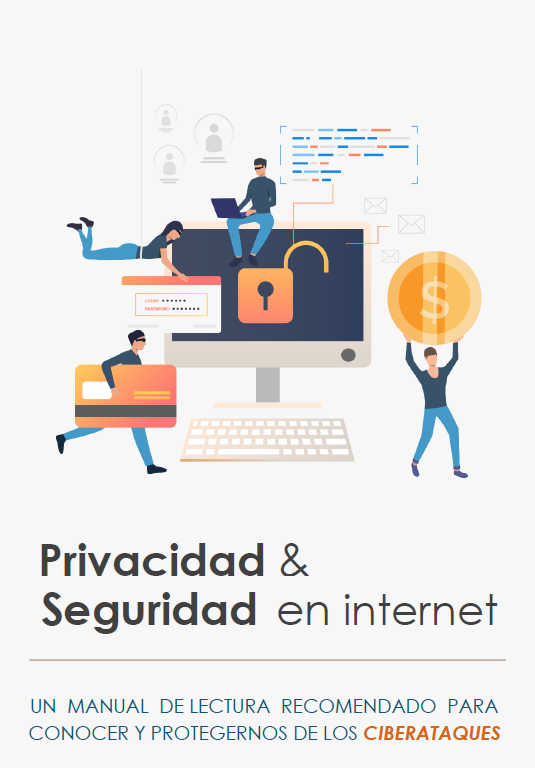
\includegraphics[width=\paperwidth]{images/cover.png}}
%\makebox[\textwidth]{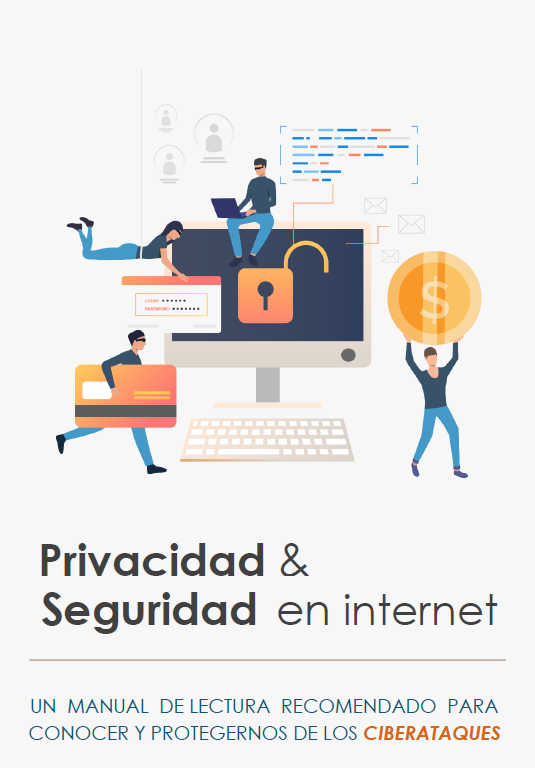
\includegraphics[width=\paperwidth]{images/cover.png}}
\end{center}
\fontsize{14}{16}
%\fontseries{b}
\selectfont





{
\hypersetup{linkcolor=}
\setcounter{tocdepth}{3}
\tableofcontents
}
\hypertarget{pruxf3logo}{%
\chapter*{Prólogo}\label{pruxf3logo}}
\addcontentsline{toc}{chapter}{Prólogo}

Este manual aglutina de manera filtrada y tamizada una amplia y detallada parte del conocimiento e información de relevancia que puedes encontrar en la web sobre privacidad y seguridad en internet, de forma ordenada y estructurada. Además encontrarás en la bibliografía todas las fuentes que han hecho posible la elaboración y documentación de este manual, para que puedas contrastar por ti mismo dichas fuentes.

Entenderás las diferencias entre los conceptos de privacidad y seguridad en internet, para que de este modo puedas hacer una buena configuración y uso de éstas.

Aprenderás buenas prácticas en la gestión de la privacidad, así como la manera más adecuada de gestionar la seguridad tanto en los equipos (PC, tables, smartphones, etc.), como en la red de datos.

Conocerás las principales amenazas que existen en el uso de las tecnologías y el mundo digital.

Y por último, pero no por ello menos importante, se abordarán otros conceptos relacionados con los ciberdelitos, la huella digital, la importancia de ser selectivos con la información online y otros aspectos más.

Para concluir, también encontrarás a lo largo del manual multitud de enlaces que te llevarán a más información ampliada sobre las temáticas, así como una extensa lista de recursos y herramientas para que puedas llevar tu privacidad y seguridad en internet al siguiente nivel.

Si quieres contribuir y ayudar a nutrir de más contenido de valor este manual, por favor, no lo dudes y ponte en contacto conmigo, estaré encantado que colaboremos. Encontrarás mis datos de contacto en el siguiente apartado \emph{sobre el autor}.

Este manual está disponible en el repositorio Github: \href{https://github.com/diegochiquero/manual-de-privacidad-y-seguridad-en-internet}{diegochiquero/manual-de-privacidad-y-seguridad-en-internet}. Y ha sido escrito en \href{http://rmarkdown.rstudio.com}{R-Markdown} empleando el paquete \href{https://bookdown.org/}{\texttt{bookdown}} cuya guia encontrarás en \citep{R-bookdown}.

Imagen portada \citep{freepik}

Esta obra está bajo la \href{https://creativecommons.org/licenses/by-nc-sa/4.0/deed.es}{licencia Creative Commons Atribución-NoComercial-CompartirIgual 4.0 Internacional}.

\begin{flushleft}
\includegraphics{images/by-nc-sa-88x31} \end{flushleft}

\hypertarget{autor}{%
\chapter*{Sobre el autor}\label{autor}}
\addcontentsline{toc}{chapter}{Sobre el autor}

\begin{flushleft}
\includegraphics[width=0.25\linewidth]{images/diego-chiquero-2020-profile} \end{flushleft}

Hola, mi nombre en Diego.

Y lo primero que me gustaría hacer, es agradecerte que hayas decidido leer este manual. Ya que éste hecho, hace que las horas de dedicación, esfuerzo, documentación, contrastación de fuentes y curación de contenidos hayan merecido la pena.

El propósito de este manual es hacerte consciente de los peligros de navegar por internet, de lo vulnerable y expuesto que puedes llegar a estar en el uso de las tecnologías y a su vez dotarte de conocimientos, consejos y herramientas para poder hacer una buena gestión de la web de manera segura y privada.

De formación académica Técnico superior en desarrollo de aplicaciones web.
Para concluir y a modo de breve presentación, haré referencia a mi extracto de Linkedin:

\begin{quote}
Apasionado de las tecnologías, el espíritu emprendedor y la programación.

Plenamente convencido que las competencias transversales pueden marcar la diferencia, que el derecho nos asiste a todos y que un mundo mejor es posible.

En continuo proceso de crecimiento personal y profesional.
\end{quote}

Diego Chiquero Mena

Puedes contactar conmigo en \href{mailto:chiquerodiego@yahoo.es}{\nolinkurl{chiquerodiego@yahoo.es}}

Más sobre mí \href{https://about.me/diegochiquero}{Diego Chiquero Mena}

\hypertarget{privacidad-y-seguridad-en-internet}{%
\chapter{Privacidad y Seguridad en Internet}\label{privacidad-y-seguridad-en-internet}}

\hypertarget{introducciuxf3n}{%
\section{Introducción}\label{introducciuxf3n}}

En estos últimos años hemos podido ver como la evolución de las IT (Tecnologías de la información) y el paso de la Web 1.0 a la Web 2.0, nos ha permitido a muchos de nosotros como usuarios interactuar los unos con los otros subiendo y compartiendo todo tipo de contenidos. La aparición de las Redes sociales ha traído con ellas, la posibilidad de publicar fotos, videos, información, comentarios, reseñas, etc. a través de cualquier dispositivo, ya sea un PC, tablet o smartphone. Y no solo eso, sino que además, también nos ha abierto un amplio abanico de posibilidades con las que podemos gestionar cuentas bancarias, hacer compras online, trámites telemáticos y un sinfín de gestiones que hasta hace tan solo unos años atrás eran difíciles de imaginar.

Además a todo lo anterior se añade este nuevo escenario hacia la web 3.0 en el que ha aumentado la exposición a la superficie digital y donde el incremento exponencial de ciberdelincuencia parece no tener freno. Es por ello que bajo estas circunstancias es cuando más debemos aprender y mejorar las destrezas digitales y hacerlas compatibles con un uso responsable, respetuoso y crítico de la tecnología, desarrollando capacidades digitales en las que un entorno, seguro, privado y sostenibles que garantice el bienestar social sea posible.

Como consecuencia de ello, el enorme conglomerado de información sensible que se encuentra disponible en internet, hace que nosotros como usuarios estemos en el punto de mira de ciberdelincuentes y expuestos a todo tipo de ciberataques. En esta línea, este manual contribuye a enseñarte, aconsejarte y proveerte de herramientas necesarias para prevenir, evitar y paliar en la medida de lo posible todos los riesgos y peligros a los que estamos expuestos en nuestro uso diario de las tecnologías.

Por lo tanto, en lo sucesivo iras viendo el porqué de la importancia de velar de manera activa por tu privacidad y seguridad en internet haciendo una buena gestión de éstas. También te ayudará a conocer y reconocer la amplia lista de ciberdelitos que actualmente están más extendidos.

En estás \href{https://oedi.es/estadisticas/}{estadísticas} públicadas por el Observatorio Español de Delitos informáticos \citep{oedi} puedes ver el porqué de cuidar tu privacidad y seguridad en internet. En ellas se expone una exhaustiva lista de ciberdelitos y sus recurrencias cronológicas.

\hypertarget{privacidad}{%
\section{Privacidad}\label{privacidad}}

La privacidad es aquello que se lleva a cabo en un ámbito reservado; en Internet podría entenderse como el control que ejercemos sobre nuestra información para limitar la cantidad de personas autorizadas a verla, así como la cantidad de contenido expuesto. Esto incluye datos personales, fotografías, documentos, etc.

Internet es una herramienta que nos permite la interacción entre dos o más personas. Siendo ejemplo de los anteriores sitios como Facebook y Twitter, Redes Sociales en donde las personas pueden compartir públicamente opiniones, noticias, sentimientos, ideas, fotografías, videos, etc. Por ello es necesario considerar que Internet es un espacio abierto al mundo, por lo tanto, cualquier acción que se haga va a tener un impacto global y permanente. Por ejemplo, imagina una publicación de la cual puedas arrepentirte (como una fotografía u opinión) no solo podrá ser vista por millones de usuarios , sino que también será prácticamente imposible de borrar completamente de la red .

También puede resultar peligroso publicar datos que puedan identificarte, como la dirección, teléfonos, lugar de estudio o trabajo, días de vacaciones, etc. Esto puede resultar todavía más complicado si posees una gran lista de amigos a los que no conoces personalmente.

Por todo lo que se ha mencionado en éstas últimas líneas, es de suma importancia que antes de publicar algo, pienses en las consecuencias que puede conllevar divulgar información sensible en sitios públicos y de los cuales no siempre se tiene un control directo \citep{privacidad}.

\hypertarget{seguridad}{%
\section{Seguridad}\label{seguridad}}

La seguridad en internet son todas aquellas precauciones que son tomadas para proteger todos los dispositivos informáticos, así como la red de internet que pueden ser afectados por delincuentes cibernéticos. Además de ser una rama de la seguridad informática que se dedica a identificar y prevenir todas las amenazas que afectan a la red de redes, siendo una de las herramientas más conocidas los antivirus \citep{seguridad}.

Entre los peligros más habituales de no hacer un buen uso de la seguridad en la red, nos encontramos, robo de datos bancarios o personales, virus informáticos, phishing, spam, etc. Pero estos no son los únicos riesgos que asechan en internet, como verás más adelante.

\hypertarget{rgpd-reglamento-general-de-protecciuxf3n-de-datos}{%
\section{RGPD (Reglamento general de protección de datos)}\label{rgpd-reglamento-general-de-protecciuxf3n-de-datos}}

El Reglamento General de Protección de Datos (RGPD) es el reglamento europeo relativo a la protección de las personas físicas en lo que respecta al tratamiento de sus datos personales y a la libre circulación de estos datos. Entró en vigor el 25 de mayo de 2016 y fue de aplicación el 25 de mayo de 2018, dos años durante los cuales las empresas, las organizaciones, los organismos y las instituciones han debido ir adaptándose para su cumplimiento. Es una normativa a nivel de la Unión Europea, por lo que cualquier empresa de la unión, o aquellas empresas que tengan negocios en ésta y que manejen información personal de cualquier tipo deberán acogerse a la misma \citep{WIKI-rgpd}.

En el pasado, el uso de datos era obtenido por omisión, en estos momentos para estar seguros de cumplir con el RGPD se ha de obtener el consentimiento inequívoco o expreso por parte del usuario.

Paralela a la RGPD europea existe una a nivel de España llamada Ley orgánica de protección de datos y garantía de los derechos digitales, recogida en el BOE \href{https://www.boe.es/buscar/doc.php?id=BOE-A-2018-16673}{Boletín Oficial del Estado} y cuyo objeto es también garantizar y proteger las libertades públicas y los derechos fundamentales de las personas físicas y en especial, su honor e integridad personal y familiar.

Entre los aspectos más significativos del RGPD cabe destacar los siguientes:

\begin{itemize}
\item
  Derecho a la portabilidad de los datos: Te da el derecho de solicitar al responsable de tus datos el traspaso de éstos a otra entidad o responsable. Un ejemplo claro es la conocida portabilidad en el mundo de la telefonía que hacen que tus datos puedas ser cedidos de una compañía a otra.
\item
  Derecho a la supresión: Es una versión mejorada de la solicitud de cancelación o eliminación de tus datos.
\item
  Derecho al olvido: Te da derecho a solicitar al responsable de tus datos la supresión o eliminación de éstos pero con un enfoque más estrecho con el ámbito digital. Desde el servicio ofrecido por \href{https://www.aepd.es/es/areas-de-actuacion/internet-y-redes-sociales/derecho-al-olvido}{AEPD} pudes acceder a los enlaces donde solicitar el derecho al olvido en \href{https://www.google.com/webmasters/tools/legal-removal-request?complaint_type=rtbf\&visit_id=637490694757326412-3626204680\&hl=es\&rd=1}{Google}, \href{https://www.bing.com/webmaster/tools/eu-privacy-request}{Bing}, \href{https://es.ayuda.yahoo.com/kb/Solicitud-para-bloquear-resultados-de-b\%C3\%BAsqueda-en-Yahoo-Search-Recursos-para-Residentes-Europeos-sln28252.html?guccounter=1\&guce_referrer=aHR0cHM6Ly93d3cuYWVwZC5lcy8\&guce_referrer_sig=AQAAAIRquvv_VPnIiAOniwOvZi_iVodzBg6yn2C0sGApxESxJWBR6RMqeNq89qO01lmI0UdIKSr3ivLxST8cTDrgIMQRF9FIda60jZQ16f8q85f-eqLvvviA02B_fephtV40QIGV7aQ8Uw0M7f_poDUONOrmeKQzbahKvnuKZCoBDBFQ}{Yahoo}, aunque desde estos últimos enlaces ya puedes acceder directamente.
\end{itemize}

\hypertarget{aviso-legal-poluxedtica-de-privacidad-y-poluxedtica-de-cookies}{%
\section{Aviso legal, política de privacidad y política de cookies}\label{aviso-legal-poluxedtica-de-privacidad-y-poluxedtica-de-cookies}}

Si una web va a realizar transacciones comerciales de la naturaleza que sea, va a gestionar datos de usuarios o hacer uso de cookies, ha de tener a disposición del usuario las políticas que más abajo se detallan. Todas estas políticas están recogidas en el RGPD del apartado anterior. Sin embargo para documentarlo con terminología más cotidiana, en este apartado nos hemos apoyado en la sección de derecho digital de la compañía IONOS by 1\&1 en su división IONOS Guía Digital.

\begin{itemize}
\item
  Aviso Legal: Se trata de un documento donde se recogen tanto el cumplimiento por parte de la entidad o empresa, conforme a las leyes vigentes en el desarrollo de su actividad, así como los datos referentes a los administradores de la misma.

  Todo proyecto de base digital u online con ánimo de lucro, ya sea a través de modelos de patrocinio, publicitarios o compra-venta de productos o servicios, requieren de un aviso legal visiblemente expuesto y a disposición de todos los usuarios. Este requerimiento está recogido en la legislación española en la Ley 34/2002 de Servicios de la Sociedad de la Información y el Comercio Electrónico \citep{IONOS-legal}.
\item
  Política de privacidad: El reglamento general de Protección de Datos de carácter personal, establece que cualquier página web que incluya un formulario de carácter personal que deban rellenar los usuarios, que incluya un correo de contacto o utilice las redes sociales desde las cuales se puede obtener información de los usuarios, está obligada a disponer de una política de privacidad \citep{IONOS-privacidad}.

  La política de privacidad se creó con la finalidad de proteger y preservar los derechos del espacio privado de las personas.
\item
  Política de cookies: Una cookie es una pequeña información enviada por un sitio web y almacenado en el navegador del usuario, de manera que el sitio web puede consultar la actividad previa del navegador. Su propósito principal es identificar al usuario almacenando su historial de actividad en un sitio web específico, de manera que se le pueda ofrecer el contenido más apropiado según sus hábitos \citep{IONOS-cookies}.

  Toda web que haga uso de cookies está obligada ponerlo en conocimiento de los usuarios y a solicitar su aceptación.

  Con respecto a la legislación de la Unión Europea sobre el consentimiento de las cookies debes saber que dicha ley dicta que los usuarios de internet deben tener la opción de poder rechazarlas, sin que por ello éste se vea perjudicado en su navegación. Esto nos lleva a señalar que el problema está en que la mayoría de los sitios web no lo cumplen. Normalmente tú como usuario en una mayor parte de las veces solo te vas a encontrar con la opción de aceptar todas las cookies o rechazarlas, en otros casos con otra opción más confusa y compleja de manejar la configuración de estás. Y en la inmensa mayoría de las ocasiones no te vas a encontrar con esa alternativa que te brinda la ley de poder rechazarlas \citep{GEN-rechazar-cookies}.
\end{itemize}

\hypertarget{derechos-arco}{%
\section{Derechos ARCO}\label{derechos-arco}}

Los derechos ARCO (Acceso, Rectificación, Cancelación y Oposición), están regulados por la Ley Orgánica de Protección de Datos y Garantía de Derechos Digitales, que has podido ver en un apartado anterior.

\begin{itemize}
\item
  Derecho al acceso: Te da derecho a conocer el uso que la entidad o responsable de tus datos esta haciendo de ellos.
\item
  Derecho a la rectificación: Te da derecho a solicitar la rectificación de tus datos.
\item
  Derecho a la cancelación: Te da derecho a solicitar la supresión de los datos que resulten inadecuados o excesivos.
\item
  Derecho a la oposición: Te da derecho a oponerte al tratamiento de sus datos personales o el cese de éstos.
\end{itemize}

Para poder ejercer estos derechos solo basta con solicitarlo a la parte responsable de tus datos, aportando fotocopia del DNI o documento equivalente, la petición que se solicita, la dirección a efectos de notificaciones y los documentos que acreditan la petición que se formula \citep{arco}.

\hypertarget{gestiuxf3n-de-la-privacidad}{%
\chapter{Gestión de la privacidad}\label{gestiuxf3n-de-la-privacidad}}

\hypertarget{gestionar-la-privacidad}{%
\section{Gestionar la privacidad}\label{gestionar-la-privacidad}}

La privacidad en Internet se refiere al control de la información personal que posee un determinado usuario que se conecta a Internet, interactuando por medio de diversos servicios en línea con los que intercambia datos durante la navegación. Por ello, en esta unidad vas a lograr aprender a gestionar la privacidad de manera inteligente, para así evitar males mayores que podrían hacer de tu vida privada un terreno en el que seguro, no te gustará estar \citep{WIKI-privacidad}.

\hypertarget{datos-personales-sensibles}{%
\section{Datos personales sensibles}\label{datos-personales-sensibles}}

Cuando se habla de datos personales sensibles en la red, se refiere a aquellos datos que están revelando información privada, como por ejemplo, el domicilio o cualquier otra información de carácter privado, costumbres o hábitos. Así como acciones que ubican o determinan a una persona en posibles situaciones futuras que pudiesen abrir una brecha de vulnerabilidad en la vida privada de ésta. Un ejemplo sería subir a la red que te vas de vacaciones, de manera que estás diciendo a los ciberdelincuentes que tu casa estará vacía.

Entrando en un terreno más técnico los datos sensibles son aquellos que, de difundirse indebidamente podrían afectar la esfera más íntima del ser humano. Ejemplos de este tipo de datos son: el origen racial o étnico, el estado de salud, la información genética, las creencias religiosas, filosóficas y morales, la afiliación sindical, las opiniones políticas y las preferencias sexuales.

Por ello, aporta solo los datos necesarios y no te expongas.

\hypertarget{oversharing-o-sobreexposiciuxf3n}{%
\section{Oversharing o sobreexposición}\label{oversharing-o-sobreexposiciuxf3n}}

El Oversharing es la sobreexposición de información personal en internet y en su mayoría en los Medios Sociales a través de tus perfiles sociales. Este hecho se presenta continuamente en la actualidad, donde los jóvenes y no tan jóvenes, publican constantemente imágenes o información personal.

De esta manera, tu vida queda totalmente expuesta y aunque el propósito de ello sea totalmente lícito e incluso plausible, estos datos, imágenes o información pueden volverse en tu contra por un uso indebido o ilícito por parte de terceros.

Este exceso de información que se puede facilitar en internet, sumado al comportamiento malicioso de otros usuarios, supone un grave riesgo que se corre cada día al señalar tu ubicación, comentar información personal o privada, colgar una imagen o video comprometedores, etc.

Esto no supone un delito en cuestión, pero puede dar lugar al chantaje, ciberacoso o robo de información personal a través de algún tipo de técnica. Además de exponerte al riesgo de un posible robo y/o suplantación de identidad \citep{AEPD-oversharing}.

\hypertarget{privacidad-en-tus-cuentas}{%
\section{Privacidad en tus cuentas}\label{privacidad-en-tus-cuentas}}

Prácticamente todo el mundo en menor o mayor medida dispone de cuentas de usuarios en todas sus aplicaciones o servicios en la red. Una de las más conocidas es la cuenta de \href{https://myaccount.google.com/data-and-personalization}{Google}, así como también la de \href{https://account.microsoft.com/account/privacy}{Microsoft} entre otras. En ambos enlaces podrás ajustar la privacidad con la que más cómodo te sientas. Además recuerda que no solo estos dos servicios disponen de estos ajustes, sino que también el resto de plataformas deben brindarte la posibilidad de que realices tu propia configuración.

En lo que respecta a las redes sociales como, \href{https://es-la.facebook.com/help/325807937506242}{Facebook}, \href{https://help.twitter.com/es/safety-and-security\#ads-and-data-privacy}{Twitter} o \href{https://es-es.facebook.com/help/instagram/196883487377501/?helpref=hc_fnav\&bc\%5B0\%5D=Ayuda\%20de\%20Instagram\&bc\%5B1\%5D=Administrar\%20tu\%20cuenta}{Instagram}, entre otras muchas más, no debes olvidar que también disponen opciones de privacidad y que en éste escenario está en juego tus datos más personales. Luego el mejor consejo es establecer una configuración privada en lugar de pública, ya que estas redes sociales no tienen por defecto, los niveles más elevados en cuanto a la protección y a la seguridad.

Con referencia a todo lo expuesto, puedes dejar la configuración de privacidad que la cuenta trae por defecto o acomodarla a tus necesidades o preferencias. Dentro de cada cuenta se encuentran todas las opciones de privacidad, como por ejemplo, historial de búsquedas, actividad de ubicación entre otras.

\hypertarget{navegaciuxf3n-privada}{%
\section{Navegación privada}\label{navegaciuxf3n-privada}}

La navegación privada es una función de privacidad que conocerás como modo incógnito o modo privado. Su principal característica es que permite a los navegadores web no almacenar información sobre la página en que navegamos.

La navegación privada te ofrece una sesión temporal que no comparte datos con el navegador, que no guarda información sobre páginas web, ni historial de navegación, caché web, contraseñas, información de formularios, cookies u otros datos de sitios web, borrando éstos y otros archivos temporales cuando finalices la sesión \citep{navegacion-privada}.

\begin{figure}

{\centering 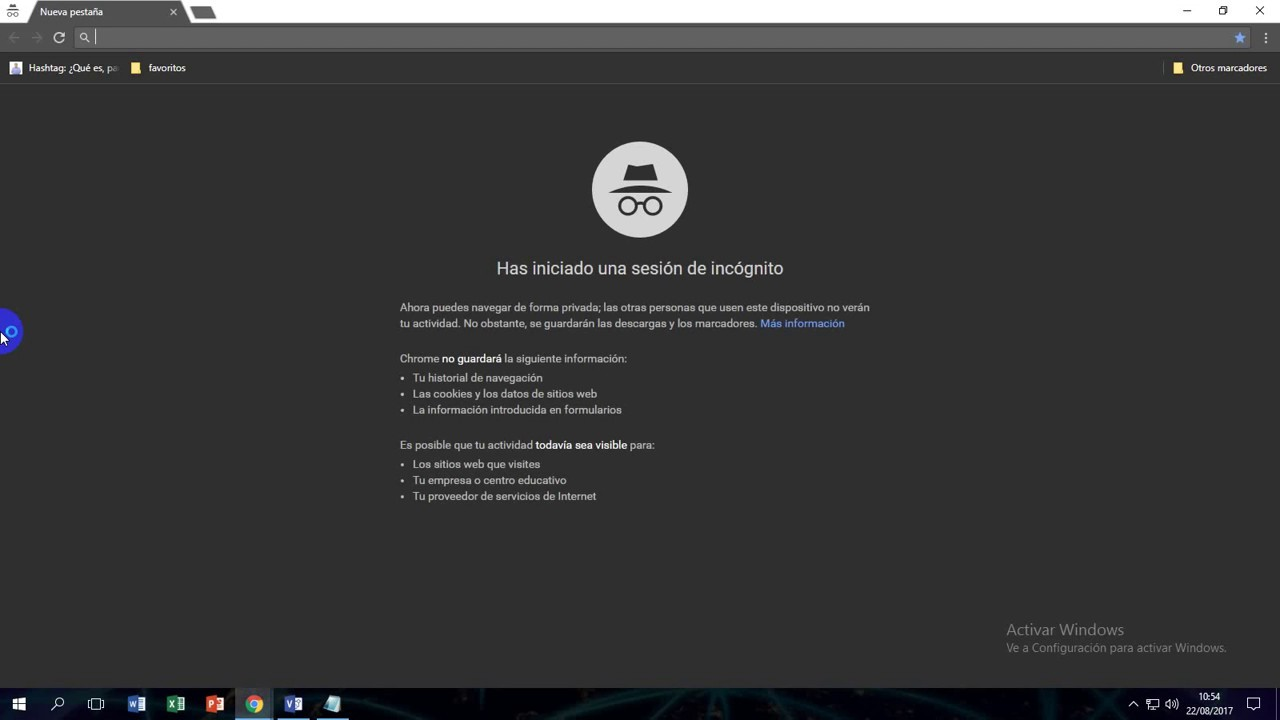
\includegraphics[width=0.75\linewidth]{images/navegacion-privada} 

}

\caption{Navegación privada navegador Google Chrome.}\label{fig:unnamed-chunk-4}
\end{figure}

Ten en cuenta que no es lo mismo navegar privadamente que navegar de forma anónima por Internet, lo que requiere de otras herramientas como \href{https://www.torproject.org/}{TOR}.

El uso de la navegación privada resulta conveniente en los siguientes supuestos:

\begin{itemize}
\tightlist
\item
  Transacciones económicas.
\item
  Utilización de un ordenador de terceros.
\item
  Obtención de resultados ``puros'' del motor de búsquedas.
\end{itemize}

También existen navegadores que protegen tu privacidad sin necesidad de activar la navegación privada, como por ejemplo, \href{https://www.epicbrowser.com/}{Epic}, \href{https://brave.com/es/}{Brave} e incluso buscadores como \href{https://duckduckgo.com/}{DuckDuckGo}.

\hypertarget{vpn-red-privada-virtual}{%
\section{VPN (Red privada virtual)}\label{vpn-red-privada-virtual}}

Otra manera más de proteger tu privacidad, es hacer uso de una VPN (son las siglas de Virtual Private Network) \citep{AVAST-vpn}.

Las VPN son una tecnología de red que permiten una extensión de tu conexión local o LAN, permitiendo conectar varios dispositivos como si se encontrasen físicamente en el mismo lugar. Entre sus ventajas está la de ofrecer una mayor privacidad al ocultar tu localización, pero también, y este el caso que nos compete, el que parezca que tu conexión esté realizándose en otro país concreto, con lo que uno se puede saltar censuras o acceder a contenidos de servicios locales.

Su principal particularidad es que se trata de una conexión segura y cifrada. Esto hace que no sea posible conocer la información que viaja en la petición que se realiza, así como tampoco la IP pública que identifica tu dispositivo, ya que la conexión se realiza a través de los muchos router VPN en diferentes ubicaciones.

Las VPN suelen ser aplicaciones o extensiones de terceros, aunque el navegador \href{https://www.opera.com/es}{OPERA} lo trae por defecto. Lo único que tendrás que hacer es activarla desde sus opciones, y se creará una conexión cifrada entre tu dispositivo y un servidor VPN para esconder tu ubicación real.

No obstante no todas las VPN son igual de eficaces y en ocasiones algunas de ellas pueden no estar funcionando todo lo bien que cabría de esperar y durante tu sesión de navegación podrían verse expuestos algunos de tus datos. Por suerte, existen herramientas como \href{https://whatleaks.com/}{What leaks?} que te permite analizar la eficacia de tu VPN a la hora de proteger tu privacidad.

\hypertarget{cookies}{%
\section{Cookies}\label{cookies}}

Una cookie es un fichero que guarda nuestro navegador, donde se almacenan pequeñas cantidades de datos, de manera que el sitio web puede consultar la actividad previa del navegador.

Su propósito principal es identificar al usuario almacenando su historial de actividad de un sitio web específico, de manera que se le pueda ofrecer el contenido más apropiado según sus hábitos. Esto quiere decir que cada vez que visitas una página web por primera vez, se guarda una cookie en el navegador con un poco de información. Luego, cuando visitas nuevamente la misma página, el servidor pide la misma cookie para arreglar la configuración del sitio y hacer la visita del usuario tan personalizada como sea posible \citep{cookies-navegador}.

Existe la opción de navegar sin cookies gracias a las sesiones privadas que tienen los distintos navegadores, como has podido ver en el apartado anterior. De esta forma no se almacenará ningún tipo de información en tu ordenador cuando navegues en una web y del mismo modo tampoco recordará nada después al volver a navegar de nuevo.

Es importante que con frecuencia elimines las cookies, ahora que sabes que manejan información privada y además ocupan espacio en tu dispositivo. Existen dos formas manuales de hacerlo. La primera de ellas es desde el menú de opciones del propio navegador y la otra es con un software específico para tal cometido, como por ejemplo \href{https://www.ccleaner.com/es-es}{Ccleaner}. Pero si quieres automatizar esta tarea, practicamente todos los navegadores disponen de una configuración para que una vez cierres el navegador se realice una limpieza de manera automática. La siguiente imagen te muestra la opción que debes buscar en el navegador Google Chrome, para ello ve al Menu del navegador, entra en Configuracíón, luego Privacidad y seguridad, a continuación Cookies y finalmente Borrar las cookies y los datos de sitios al salir de Chrome, pero debes tener en cuenta que las ubicaciones pueden variar con las actualizaciones. Si usas otro navegador puede ser que varíe la ruta de acceso, pero a grandes rasgos suelen ser muy parecidas y también se acceden a ellas a través del menú de opciones.

\begin{figure}

{\centering 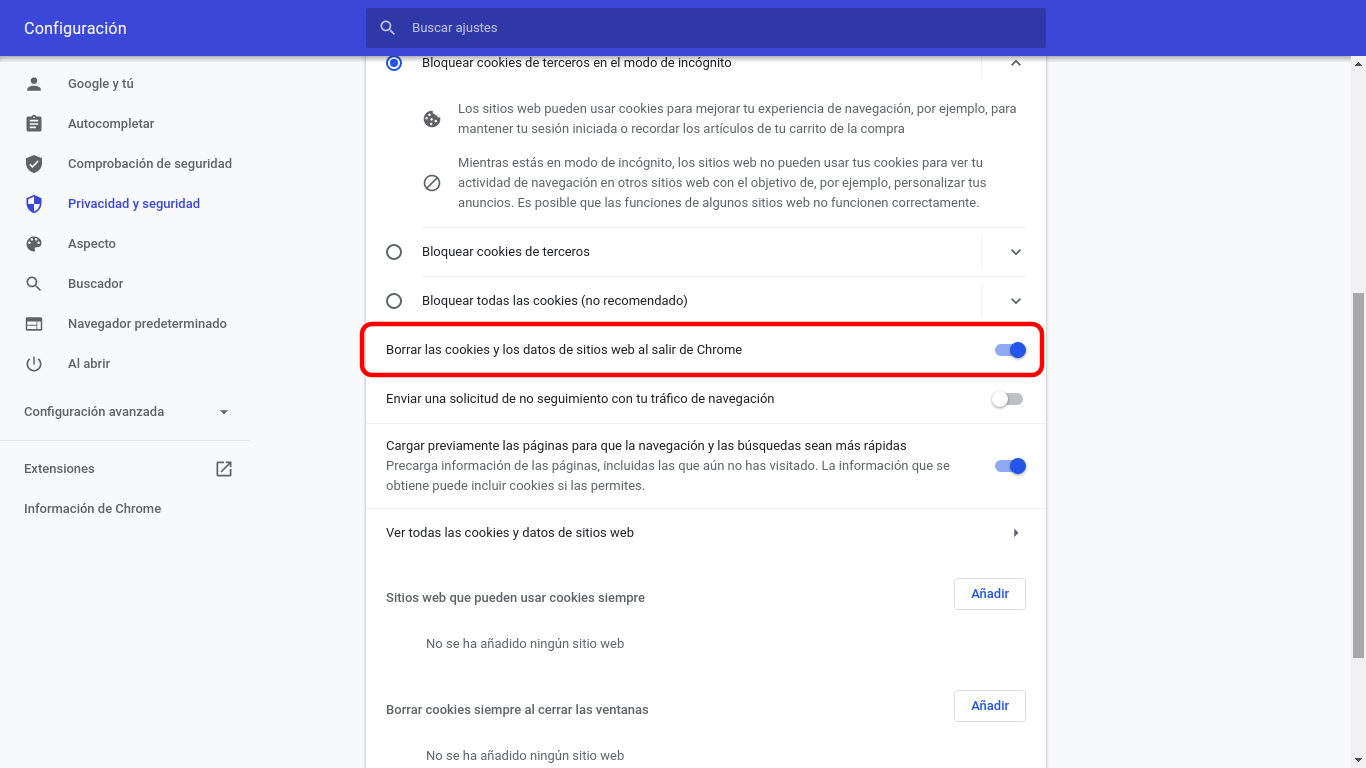
\includegraphics[width=0.75\linewidth]{images/borrado-cookies-cierre-navegador} 

}

\caption{Eliminar cookies automáticamente al cerrar Google Chrome.}\label{fig:unnamed-chunk-5}
\end{figure}

Por otro lado si quieres deshacerte de la incómoda notificación de cookies de las web, puedes instalar en el navegador el plugin \href{https://www.i-dont-care-about-cookies.eu/}{I don't care about cookies} o este otro \href{https://ninja-cookie.com/}{Ninja cookie}, elige el que más te guste.

Si quieres más información detallada sobre las cookies visita este enlace \href{https://www.osi.es/es/actualidad/blog/2019/09/11/por-que-borrar-las-cookies-del-navegador}{por qué borrar las cookies} y este otro \href{https://www.osi.es/es/actualidad/blog/2018/07/18/entre-cookies-y-privacidad}{tipos de cookies, cofiguración y consejos} de la Oficina de Seguridad del Internauta donde las analizan con más detalle.

\hypertarget{permisos-cuxe1mara-micruxf3fono-y-localizaciuxf3n.}{%
\section{Permisos cámara, micrófono y localización.}\label{permisos-cuxe1mara-micruxf3fono-y-localizaciuxf3n.}}

Una práctica muy saludable en el uso de la cámara o webCam e incluso el micrófono, es tenerla tapada cuando no la estés usando y si no fijate en la foto que se muestra a continuación que le tomaron a Mark Zuckerberg.

\begin{figure}

{\centering 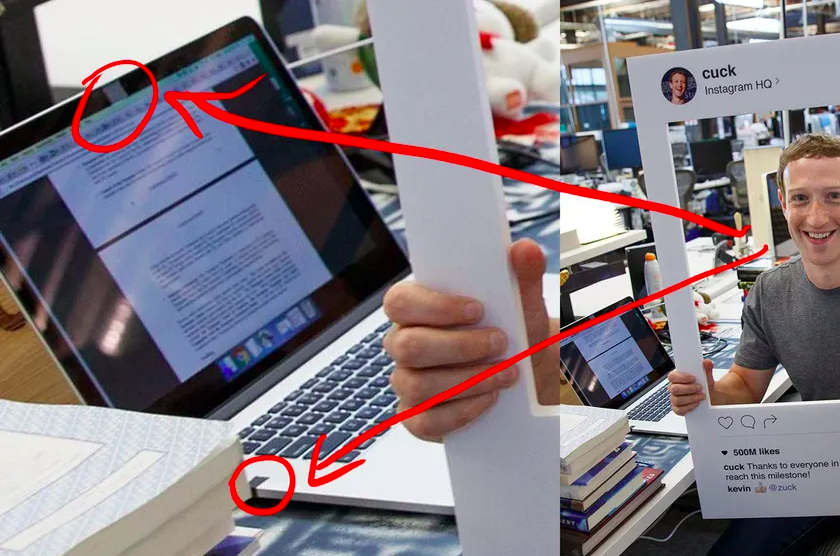
\includegraphics[width=0.75\linewidth]{images/webca-mark-zuckerberg} 

}

\caption{WebCam y micrófono del ordenador tapados.}\label{fig:unnamed-chunk-6}
\end{figure}

Para tener el control total sobre las funcionalidades de cámara, micrófono y ubicación, debes establecer los permisos en la opción de Preguntar, lo verás más claramente en la imagen que se muestra más abajo. Para establecer estos parámetros existen dos maneras de hacerlo, uno de ellas es a través de la opciones que te da el menú de configuración del propio navegador, y para ello debes ir a Menú navegador, buscar Configuracíón, después Privacidad y seguridad, a continuación Configuración de sitios web y finalmente Permisos. Como ya se indicó en el caso de borrado de cookies automático, debes tener en cuenta que las ubicaciones pueden variar con las actualizaciones que reciba el navegador.

\begin{figure}

{\centering 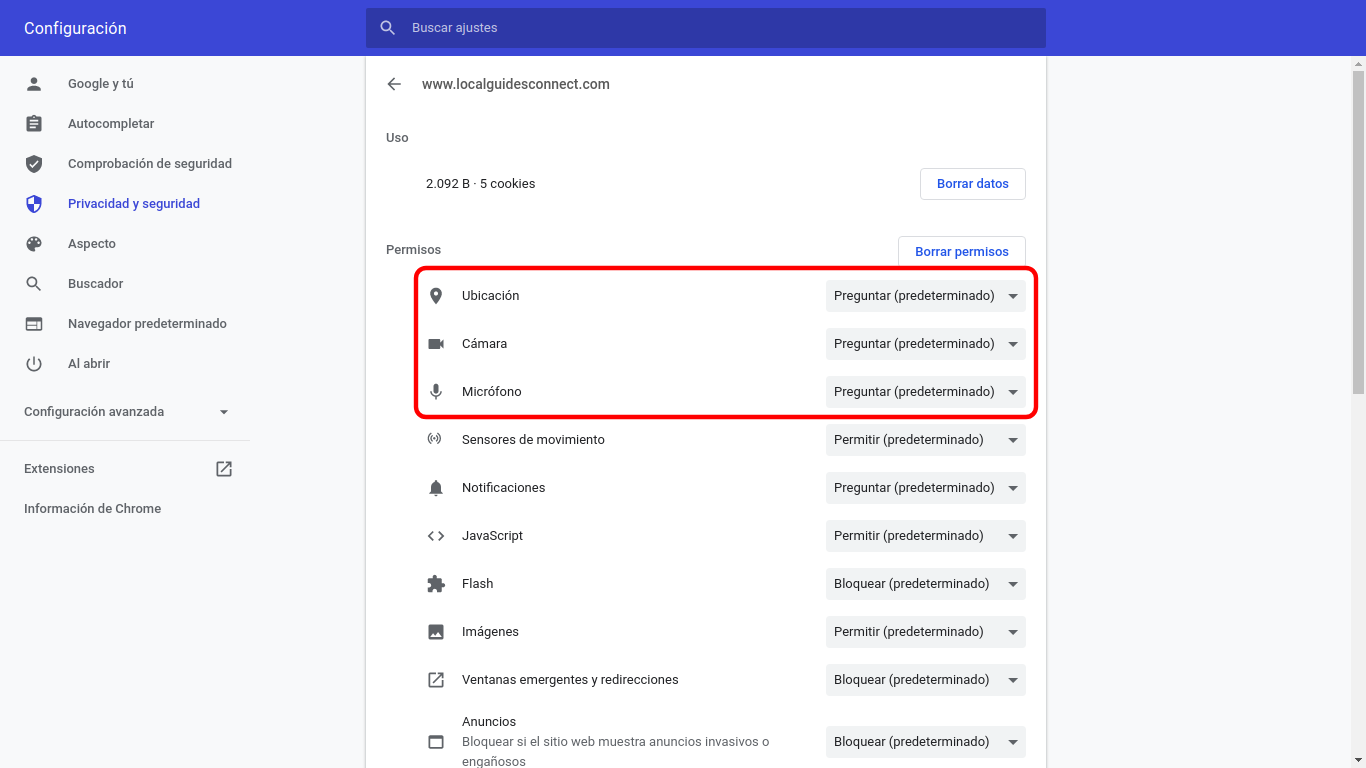
\includegraphics[width=0.75\linewidth]{images/ajuste-permisos} 

}

\caption{Ajustes permisos cámara, micrófono y ubicación desde el menú de opciones del navegador.}\label{fig:unnamed-chunk-7}
\end{figure}

Aunque estos permisos son los más importantes cuando navegas por internet, si te fijas en la figura 2.4 verás que no son los únicos y que entre éstos se encuentran los de notificaciones o los de ventanas emergentes entre otros.

La otra forma es más sencilla e incluso te permite cambiar los permisos directamente desde el navegador sin tener que ir al menú de opciones y esto lo tienes haciendo click en el candado de la barra de direcciones. Se trata del mismo candado que nos acredita que estamos ante una web segura. Puedes verlo en la siguiente imagen.

\begin{figure}

{\centering 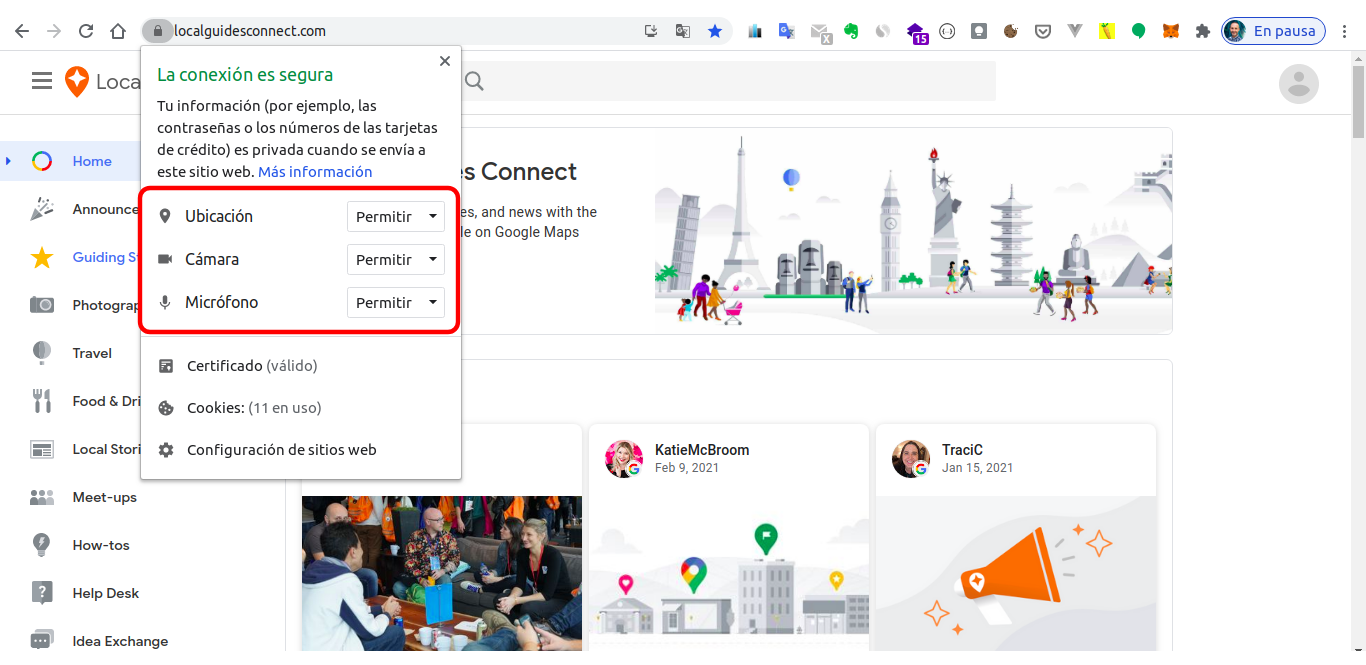
\includegraphics[width=0.75\linewidth]{images/ajuste-permisos-desde-navegador} 

}

\caption{Ajustes permisos cámara, micrófono y ubicación desde el candado de la barra de direcciones.}\label{fig:unnamed-chunk-8}
\end{figure}

Para concluir, no debes olvidar que con las aplicaciones móviles sucede lo mismo, y que puedes gestionarlos de igual manera desde ajustes del dispositivo. Visita los siguientes enlaces dependiendo de tu smartphone, \href{https://support.google.com/android/answer/9431959?hl=es}{cambiar los permisos de las aplicaciones en teléfonos Android} o \href{https://support.apple.com/es-es/guide/iphone/iph251e92810/ios}{controlar el acceso a la información en las apps en el iPhone}. En el siguiente enlace, \href{https://www.osi.es/sites/default/files/docs/c5-eg-permisos-apps-riesgos.pdf}{permisos aplicaciones móviles} encontrarás una tabla con los permisos y los riesgos que entrañan.

\hypertarget{la-nube}{%
\section{La nube}\label{la-nube}}

Como ya sabrás el almacenamiento en la nube, es el almacenamiento de datos en servidores por lo general aportados por terceros y que gracias a esto, puedes disponer de ellos desde cualquier lugar y dispositivo, con solo tener conexión a internet y conectarte al servicio donde están alojados tus datos. De esta manera ya no es necesario llevar contigo el dispositivo físico donde tienes almacenada tu información. Algunos de estos servicios más conocidos son \href{https://www.google.com/intl/en_in/drive/}{Google drive}, \href{https://www.microsoft.com/en-us/microsoft-365/onedrive/online-cloud-storage}{One drive} o \href{https://www.dropbox.com/}{Dropbox} entre otros.

Antes de decidirte por cuál de los proveedor de servicio en la nube debes decantarte, ten en cuenta los siguientes:

\begin{itemize}
\item
  Donde va a estar ubicada tu información. Esto te permitirá conocer la legislación y
  garantías de protección de tus datos en el país donde se encuentren.
\item
  Saber si la plataforma comparte información con terceros o no.
\item
  Si la web cuenta con certificado digital y es accesible mediante https.
\item
  Mecanismos de cifrado, ya que éstos maximizan la seguridad de los datos.
\item
  Políticas de privacidad.
\end{itemize}

De otro lado también puedes tomar tus propias medidas de seguridad cifrando tu datos antes de subirlos. Para ello puedes usar esta herramienta llamada \href{https://cryptomator.org/}{cryptomator}.

En este enlace encontrarás un estudio completo de los diferentes \href{https://www.osi.es/sites/default/files/docs/osi_servicios_nube.pdf}{servicios de almacenamiento en la nube} y sus características.

A la hora de compartir tus datos alojados en la nube debes tener en cuenta que solo es recomendable compartirlos con personas de confianza, ya que de lo contrario podrían hacer un mal uso de ello, o simplemente una mala gestión que provoque la pérdida de la información.

\hypertarget{correo-electruxf3nico-y-apps-de-mensajeruxeda}{%
\section{Correo electrónico y apps de mensajería}\label{correo-electruxf3nico-y-apps-de-mensajeruxeda}}

El correo electrónico es uno de los servicios web que más se suele utilizar. Por ello debes saber que muchos de lo gestores de emails que son utilizados a diario, no aplican estrictas políticas de privacidad, por lo que tus correos podrías ser leídos y rastreados no solo por terceros con intenciones poco saludables sino también por éstos mismos servicios de correo.

Esto no tiene por que ser un inconveniente si no envías información sensible, pero si no es el caso quizá preferirías usar un gestor de correos que sí te garantice una privacidad completa en tus envíos. De ser este tu caso puedes usar \href{https://protonmail.com/}{Protonmail}, \href{https://tutanota.com/es/}{Tutanota} o \href{https://www.fastmail.com}{Fastmail} que si tienen en cuenta este aspecto, aunque no son los únicos. En el siguiente enlace tienes una lista de otras \href{https://blogthinkbig.com/alternativas-gratuitas-gmail-outlook-privacidad}{alternativas de emails privadas}.

Si por el contrario prefieres ser tu quien gestiones esa capa de privacidad adicional, puedes optar por hacer uso de otras herramientas de encriptado que podrás ver en este artículo de \href{https://www.osi.es/es/actualidad/blog/2019/07/31/como-encriptar-y-proteger-tu-correo-electronico}{cómo encriptar y proteger tu correo electrónico}.

Si además quieres saber si tu cuenta de correo o tu número de teléfono han sido comprometidos, puedes saberlo a través de la siguiente plataforma \href{https://haveibeenpwned.com/}{haveibeenpwned}.

Con respecto a las aplicaciones de mensajería instantánea debes tener en cuenta que sucede lo mismo que con los correos electrónicos. A pesar que la mayoría de ellas, incluida la más popular de todas (whatsApp) disponen de capas de privacidad que la hacen confiable, a veces no podemos estar totalmente seguros de no estar sometidos a un seguimiento por parte de éstas. Es por ello, que las aplicaciones como \href{https://telegram.org/}{telegram} y \href{https://signal.org/es/}{signal} nacen con el propósito de no inmiscuirse en el uso que haces de la aplicación.

\hypertarget{he-decidido-vender-o-donar-mi-dispositivo}{%
\section{He decidido vender o donar mi dispositivo}\label{he-decidido-vender-o-donar-mi-dispositivo}}

Si estás pensando en vender o quizá donar cualquiera de tus dispisitivos, ya sea un disco duro externo, el ordenador o portátil, un USB o cualquier otro dispositivo que contenga almacenamiento, asegurate primero de eliminar totalmente todo el contenido. Para ello utiliza software de borrado definitivo, ya que un simple formateado no borrará la información. El borrado solo se completa cuando se reescribe sobre la anterior información, es por esto que un formateo solo te hace constar que el espacio esta disponible, pero el contenido, aunque oculto, sigue estando ahí. Esto quiere decir que con software avanzado y específico los ciberdelicuentes podrían recuperar todo el contenido \citep{XATAKA-borrado-almacenamiento}.

Si quieres más recomendaciones sobre como actuar en este supuesto, te recomiendo que leas la siguiente entrada \href{https://www.osi.es/es/actualidad/blog/2019/10/09/sabias-que-2-de-cada-5-dispositivos-vendidos-contienen-informacion}{¿Sabías que 2 de cada 5 dispositivos vendidos contienen información personal?}.

Algunas herramientas de borrado definitivo son:

\begin{itemize}
\item
  \href{https://eraser.heidi.ie/}{Eraser}
\item
  \href{https://www.diskwipe.org/download.php}{Disk wipe}
\end{itemize}

\hypertarget{gestiuxf3n-de-la-seguridad-en-equipos-fuxedsicos}{%
\chapter{Gestión de la seguridad en equipos físicos}\label{gestiuxf3n-de-la-seguridad-en-equipos-fuxedsicos}}

\hypertarget{gestionar-la-seguridad-en-los-equipos}{%
\section{Gestionar la seguridad en los equipos}\label{gestionar-la-seguridad-en-los-equipos}}

Para poder tener la tranquilidad de que tus equipos tales, como el ordenador, la tablet, el smartphone, el router, etc., estén a salvo de ataques o pérdidas de datos, entre otras, debes mantener una seguridad robusta y confiable en tus equipos.

A lo largo de esta unidad veras que debes hacer y las precauciones que debes tomar para que tus equipos e información estén seguros y a salvo de ciberataques.

\hypertarget{equipo-local-y-dispositivos-muxf3viles}{%
\section{Equipo local y dispositivos móviles}\label{equipo-local-y-dispositivos-muxf3viles}}

Una cuenta de usuario es el conjunto de información perteneciente a un usuario concreto. De esta forma indica al sistema operativo los archivos y carpetas a los que dicho usuario tiene acceso así como la posibilidad de realizar cambios y configuraciones personales \citep{OSI-cuentas}.

Las pautas de seguridad que vas a ver a continuación te van a ser útil, tanto para ordenadores como cualquier tipo de dispositivo móvil, smartwatch y demás.

Todos los equipos informáticos funcionan con una cuenta de usuario, única y personal. Luego una vez, hayas creado la tuya, solo tú debes hacer uso y disfrute de ella. En los ordenadores personales existe la posibilidad de crear varias cuentas de usuarios. Una vez éstas están creadas solo son accesibles mediante contraseña y aunque solo sirva para no olvidarlo, recuerda que una contraseña nunca debe ser de compartida.

Desde aquí podrás acceder a cómo \href{https://support.microsoft.com/es-es/windows/crear-una-cuenta-de-administrador-o-de-usuario-local-en-windows-10-20de74e0-ac7f-3502-a866-32915af2a34d}{crear cuenta de usuario en windows} o \href{https://support.apple.com/es-es/guide/mac-help/mtusr001/mac\#:~:text=A\%C3\%B1adir\%20un\%20usuario,en\%20\%E2\%80\%9CUsuarios\%20y\%20grupos\%E2\%80\%9D.\&text=Si\%20el\%20candado\%20situado\%20en,bajo\%20la\%20lista\%20de\%20usuarios}{crear cuenta de usuario en Mac}.

Si tu equipo es compartido con varias personas, puede que te interese crear distintas cuentas de usuarios con distintos niveles de privilegios. Si no las gestionas
adecuadamente, corres el riesgo de:

\begin{itemize}
\item
  Que terceros puedan acceder a tus archivos y eliminar/modificar información personal, como imágenes, música, documentos importantes, etc.
\item
  Modificar configuraciones de seguridad o usabilidad de tu sistema, como, por ejemplo, desactivar el antivirus o firewall.
\item
  Conectarse a determinados servicios con tus credenciales, como el correo electrónico o red social.
\end{itemize}

Además puedes gestionar las \href{https://support.microsoft.com/es-es/windows/las-opciones-de-inicio-de-sesi\%C3\%B3n-de-windows-10-y-la-protecci\%C3\%B3n-de-la-cuenta-7b34d4cf-794f-f6bd-ddcc-e73cdf1a6fbf}{opciones de inicio de sesión en windows} y las \href{https://support.apple.com/es-es/guide/mac-help/mtusr005/mac}{opciones de inicio de sesión en Mac} lo que te permitirá tener un mayor control sobre tu inicio de sesión.

\begin{figure}

{\centering 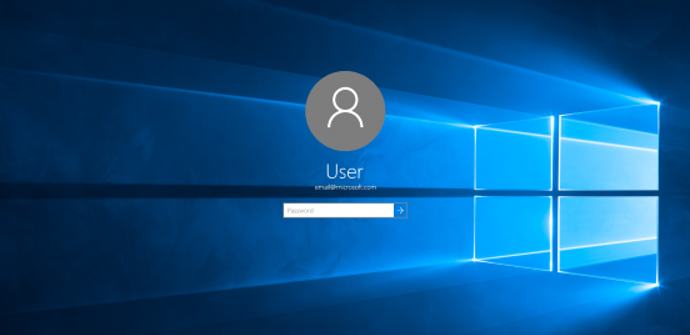
\includegraphics[width=0.75\linewidth]{images/cuenta-usuario-windows-10} 

}

\caption{Cuenta de usuario windows 10.}\label{fig:unnamed-chunk-9}
\end{figure}

\hypertarget{router}{%
\section{Router}\label{router}}

Un router es un dispositivo que proporciona conectividad a nivel de red. Su función principal consiste en enviar o encaminar paquetes de datos de una red a otra, es decir, interconectar subredes, entendiendo por subred un conjunto de máquinas IP que se pueden comunicar. Además de ser el dispositivo que nos proporciona un punto de acceso Wi-Fi

Dispone de varios niveles de seguridad y estándares de cifrado, para que nadie pueda acceder a nuestra red y poder alcanzar cualquier dispositivo a través d la Wi-Fi.

Ordenados de menor a mayor grado de cifrado:

\begin{itemize}
\tightlist
\item
  \href{https://es.wikipedia.org/wiki/Wired_Equivalent_Privacy}{WEP} (Wired Equivalent Privacy)
\item
  \href{https://es.wikipedia.org/wiki/Wi-Fi_Protected_Access}{WPA} (Wi-Fi Protected Access)
\item
  \href{https://es.wikipedia.org/wiki/WPA2}{WPA2} (Wi-Fi Protected Access 2)
\item
  \href{https://es.wikipedia.org/wiki/WPA3}{WPA3} (Wi-Fi Protected Access 3)
\end{itemize}

Es importante que uses un nivel de seguridad WPA2 como mínimo, con el que vas a poder establecer una contraseña de hasta 63 caracteres en lugar de los máximos 29 de la WEP.

Para establecer una capa más de seguridad puedes realizar un \href{https://es.wikipedia.org/wiki/Filtrado_MAC}{filtrado MAC} (Media Access Control). Un filtrado MAC consiste en la creación de una lista de dispositivos que tienen permiso para acceder al router, a pesar de que un tercero haya podido obtener la clave wifi.

Es igualmente importante que cambies la clave que el router trae por defecto. Este enlace te llevará a un \href{https://bandaancha.eu/generador-claves-wifi}{generador de claves Wi-Fi} donde podras crear de forma automática una clave Wi-Fi segura y robusta.

También es una buena práctica cambiar el nombre que la Wi-Fi trae por defecto, esto despistará a aquellos que puedan tener una lista de claves de acceso de las diferentes operadoras que existen en el mercado.

Otro aspecto a tener en cuenta es deshabilitar la opción \href{https://es.wikipedia.org/wiki/Wi-Fi_Protected_Setup}{WPS} (Wifi Protected Setup) en el router. Esta función te permite conectar el ordenador o dispositivo a la Wi-Fi del router sin tener que escribir la contraseña cuando eliges tu red Wi-Fi desde el dispositivo. Se trata de un botón físico que traen algunos router y que al pulsarlo conecta el dispositivo de forma automática. Esta funcionalidad es muy práctica pero conlleva el riesgo de que cuando pulsas este botón estás abriendo la Wi-Fi, lo que significa que inhabilitas todas las medidas de seguridad que tengas configuradas para la conexión. Si decides deshabilitarla puedes hacerlo desde la configuración de tu router y normalmente vas a encontrarlo en los apartados Wireless o Network de la interfaz web \citep{XATAKA-wps}.

Para realizar cualquiera de las configuraciones propuestas en este apartado va a necesitar acceder a la interfaz de tu router y para ello, necesitarás saber la dirección IP de acceso. Esta te será facilitada por tu operador.

Si quieres una buena guía para conocer a fondo los entresijos del router pasate por \href{https://www.osi.es/sites/default/files/docs/guia_router/osi-guia-tu-router-tu-castillo.pdf}{tu router tu castillo}.

\hypertarget{actualizaciones}{%
\section{Actualizaciones}\label{actualizaciones}}

Las actualizaciones de seguridad o parches son elaboradas por los desarrolladores y fabricantes de productos informáticos. Estos pueden tardar desde un día hasta meses para publicar un parche, en función del tipo de vulnerabilidad, dispositivos a los que afecte y otros criterios. Aunque también se realizan para mejoras de otras naturalezas, como, rendimiento, productividad, etc.

Tener actualizados los dispositivos es una medida más de seguridad. Para ello debes actualizarlos cada vez que el dispositivo lo solicita o en su defecto buscar una actualización disponible.

Las actualizaciones no solo corresponden al Hardware (ordenadores, smartphones, etc.), sino que también han de ser realizados en el software (programas), navegadores, antivirus, etc.

La principal función de las actulizaciones son las de mejorar tanto la funcionalidad como la seguridad de los dispositivos o software \citep{OSI-actualizaciones}.

\hypertarget{antivirus-antimalware-antispyware-y-firewall}{%
\section{Antivirus, antimalware, antispyware y firewall}\label{antivirus-antimalware-antispyware-y-firewall}}

Aunque a priori pudiese parecer lo mismo, los antivirus, antimalware, antispyware y firewall, cumple funciones diferentes, pero con un mismo fin, mantener la seguridad de tus equipos. La mayoría de estos tipos de software los puedes encontrar en dos modalidades: gratuita y de pago \citep{software-seguridad}.

\begin{itemize}
\item
  Antivirus: Es un programa que detecta la presencia de virus informáticos (software malicioso que altera el funcionamiento normal del ordenador sin que el usuario lo sepa o consienta) y los elimina o repara. Algunos ejemplos de antivirus son: \href{https://www.avira.com/es}{Avira}, \href{https://www.avast.com/es-es/index\#pc}{Avast}, \href{https://www.avg.com/es-es/homepage\#pc}{AVG}, \href{https://www.virustotal.com/gui/}{Virus Total} (online), entre muchos más.
\item
  Firewall o cortafuegos: Es una parte de la red o el sistema que se realiza para bloquear accesos no autorizados y permitiendo los que sí lo están. Se pueden hacer por medio de software o hardware, y permiten una mayor protección a las redes, especialmente importante en empresas que cuentan con datos que han de ser bien protegidos. El \href{https://en.wikipedia.org/wiki/Windows_Firewall}{firewall} más conocido es el Windows.
\item
  Antispyware: Es un conjunto de herramientas que sirven para prevenir y eliminar Spywares (espías o programas que recopilan información del ordenador para transmitirla a otras personas sin el consentimiento ni conocimiento del propietario del ordenador). Algunos ejemplos de antispyware son: \href{https://www.safer-networking.org/}{SpyBot}, \href{https://www.superantispyware.com/}{SuperAntiSpyware}, \href{https://www.brightfort.com/spywareblaster.html}{SpywareBlaster}.
\item
  Antimalware: Es un software encargado de eliminar el software malicioso (malicious-software, malware) del ordenador tras un minucioso análisis del sistema. Algunos ejemplos de antimalware son: \href{https://www.infospyware.com/antimalware/hijackthis/}{HiJackThis}, \href{https://www.malwarebytes.com/}{Anti-malware}.
\end{itemize}

Dependiendo de las necesidades pueden ser usados uno o varios, ya que son complementarios entre sí.

Antes de decidir que herramientas de las anteriormente expuestas va a usar, puedes hacer una búsqueda e informarte sobre las opciones disponibles, ya que existen soluciones de todo tipo y para todos los gustos, gratuitas, de pago, para ordenadores, para smartphones. Desde la \href{https://www.osi.es}{Oficina de Seguridad del Internauta} ponen a tu disposición este \href{https://www.osi.es/es/herramientas-gratuitas?herramienta_selec\%5B0\%5D=115}{listado de Antivirus gratuitos}, para que puedas elegir el que mejor se adapte a tus necesidades. Pero no olvides nunca de asegurarte muy bien que estás ante un producto legítimo y descargarlo siempre de la web oficial.

Cabe destacar que Windows de un tiempo aquí ya trae de manera nativa su propio antivirus conocido como \href{https://www.microsoft.com/es-es/windows/comprehensive-security}{Windows Defender}.

\hypertarget{copias-de-seguridad}{%
\section{Copias de seguridad}\label{copias-de-seguridad}}

Una copia de seguridad o backup en informática es una copia de los datos originales que se realiza con el fin de disponer de un medio para recuperarlos en caso de su pérdida. Las copias de seguridad son útiles ante distintos eventos y usos, como por ejemplo, recuperar los sistemas informáticos o datos de una posible catástrofe informática, natural o intensionada, restaurar una pequeña cantidad de archivos que pueden haberse eliminado accidentalmente, corrompido o infectado por un virus informático u otras posibles causas \citep{WIKI-copias-seguridad}.

Simplificando el sistema de copias de seguridad que en algunas ocasiones puede llegar a ser complejo, están los siguiente:

\begin{itemize}
\item
  Completas: Del sistema operativo completo, de esta forma al restaurar la copia, dispondremos de nuevo de toda la configuración a nivel de S.O., software instalado, carpetas y archivos. Para este cometido vamos a necesitar de programas de terceros, algunos de ellos con versiones gratuitas y de pago, ejemplo de estos son: \href{https://www.acronis.com/}{Acronis}, \href{https://www.aomeitech.com/}{AOMEI}, \href{https://www.easeus.com/}{EaseUS}. Aunque más abajo verás que también pueden hacerse nativamente.
\item
  Parciales: En este escenario lo que se hace es salvaguardar las carpetas y archivos personales. Como por ejemplo, carpetas con fotografías, documentos personales y demás.
\end{itemize}

Y las copias pueden ser mantenidas:

\begin{itemize}
\item
  En almacenamientos externos: Tales como disco duros externos, DVD, entre otros. De esta forma podemos custodiarlos a buen recaudo.
\item
  En la nube: Estos son servicios de terceros accesibles online, ejemplo de ello son: \href{https://www.backblaze.com/home-1.html}{BackBlaze}, \href{https://www.carbonite.com/}{Carbonite}, siendo estos especializados en backups. Pero si tus copias de seguridad se limitan a tus carpetas y archivos personales puedes usar un servicio en la nube, como \href{https://www.google.com/intl/en_in/drive/}{Google Drive}, \href{https://www.microsoft.com/en-us/microsoft-365/onedrive/online-cloud-storage}{Onedrive} o \href{https://www.dropbox.com/}{Dropbox}.
\end{itemize}

Las copias de seguridad debes realizarlas con la frecuencia que sea necesaria para garantizar tu nivel de seguridad \citep{tipos-copia-seguridad}.

Puedes crear una copia de seguridad de tu sistema operativo fácilmente ya que tanto Windows como Mac traen esta opción de forma nativa, solo necesitaras disponer de un dispositivo externo de almacenamiento en el que puedas guardar la copia con espacio de almacenamiento suficiente. Para Windows tienes la guía en el siguiente enlace de como \href{https://support.microsoft.com/es-es/windows/realizar-y-restaurar-una-copia-de-seguridad-del-pc-ac359b36-7015-4694-de9a-c5eac1ce9d9c}{realizar y restaurar una copia de seguridad del PC}, y para los dispositivos Apple la guía la encontrarás en \href{https://support.apple.com/es-es/mac-backup}{cómo hacer copias de seguridad en Mac}.

Una práctica muy recomendable a la hora de hacer copias de seguridad es seguir la estrategia 3-2-1 \citep{INCI-copia-3-2-1} y que consiste en:

\begin{itemize}
\item
  Mantener 3 copias de seguridad: una principal con la que trabajar y dos de backups.
\item
  Mantener la información en 2 tipos de almacenamiento distintos, por ejemplo, en un disco duro y en la nube.
\item
  Mantener 1 copia de seguridad fuera de nuestra casa.
\end{itemize}

Las copias de seguridad no son solo exclusivas de los PCs o portátiles, sino que también debes contemplarlas en tus dispositivos móviles. Android pone a tu dispoción el recurso de cómo \href{https://support.google.com/android/answer/2819582?hl=es\&visit_id=637514255756661953-3969236140\&rd=1}{crear copias de seguridad o restaurar datos de un dispositivo Android} y Apple el de \href{https://support.apple.com/es-es/HT203977}{cómo hacer una copia de seguridad del iPhone, iPad y iPod touch}.

Es muy importante que dispongas de copias de seguridad, pero igualmente de importante es que conozcas la salud de los dispositivos de almacenamientos que usas. Para ello existe software específico que realiza diagnósticos e incluso algunos tienen sistemas de reparación. De esta forma podrás saber si debes cambiar el dispositivo o no, antes de quedar en la estacada.

Software de diagnóstico y/o reparación de unidades de almacenamiento:

\begin{itemize}
\item
  \href{https://crystalmark.info/en/software/crystaldiskinfo/}{CrystalDisk}: Diagnóstico de discos HDD.
\item
  \href{https://www.hdsentinel.com/}{HdSentinel}: Diagnóstivo y reparación de discos HDD.
\item
  \href{https://hddscan.com/}{HDDScan}: Diagnóstico discos de HDD, SSD y memorias USB (pendrives).
\item
  \href{http://mikelab.kiev.ua/index_en.php?page=PROGRAMS/chkflsh_en}{Check Flash}: Diagnóstico de memorias USB (pendrives).
\end{itemize}

Por otro lado, si has borrado accidentalmente información y tu copia de seguridad no esta totalmente actualizada, quizá te interese saber que también existe software de recuperación de datos eliminados, siempre y cuando no haya pasado el suficiente tiempo para que la información eliminada haya sido reescrita. Recuerda que la información eliminada solo se produce de forma definitiva cuando se reescribe dicha información.

Aunque este último apunte no esta estrechamente relacionado con la seguridad en equipos físicos, que es el tema que se trata en esta unidad, nunca esta de más saber que tienes esta opción, para poder recuperar datos perdidos.

Para recuperar tu información dispones de software como:

\begin{itemize}
\item
  \href{https://www.ccleaner.com/recuva}{Recuba}: PC.
\item
  \href{https://www.wisecleaner.com/wise-data-recovery.html}{Wise Cleaner}: PC.
\item
  \href{https://play.google.com/store/apps/details?id=com.mediarecovery.deletedvideorecovery.deletedaudiorecovery\&hl=es}{Videos y audios Recovery}: Smartphone.
\item
  \href{https://play.google.com/store/apps/details?id=com.file.recovery.data.recovery.deletedfilerecovery}{File Recovery}: Smartphone.
\end{itemize}

\hypertarget{cifrado-o-encriptado-de-unidades-de-almacenamiento}{%
\section{Cifrado o encriptado de unidades de almacenamiento}\label{cifrado-o-encriptado-de-unidades-de-almacenamiento}}

Cifrar o encriptar tus discos duros ya sean externos o internos del ordenador o el encriptado de un simple Pendrive o USB es cada día más necesario para protegernos contra los amigos de lo ajeno, ya que aunque te sustrayecen el ordenador o cualquier otro dispositivo, no podrían acceder a la información puesto que se encuentra bajo esta capa de seguridad robusta que es la encriptación.

El cifrado de dispositivos es una tecnología que cifra todos los datos almacenado en discos duros o cualquier otro dispositivo de almacenamiento externo, con sofisticadas funciones matemáticas recogidas en lo que se conoce como \href{https://es.wikipedia.org/wiki/Criptografía}{criptografía}. De manera que para poder acceder a la información almacenada en el disco duro o pendrive en necesario tener la contraseña o clave de acceso \citep{cifrado}.

Exiten varias herramientas en el mercado para este cometido como las detalladas a continuación:

\begin{itemize}
\item
  \href{https://docs.microsoft.com/es-es/windows/security/information-protection/bitlocker/bitlocker-overview}{BitLocker}. Software nativo del sistema operativo Windows.
\item
  \href{https://support.apple.com/es-es/HT204837}{FileVault}. Software nativo del sistema operativo de macOS.
\item
  \href{https://www.veracrypt.fr}{Veracrypt}.
\item
  \href{https://diskcryptor.org/}{Diskcryptor}.
\item
  \href{https://www.comodo.com/home/internet-security/disk-encryption.php}{Comodo Disk Encryption}.
\end{itemize}

También tienes a tu dispoción el siguiente enlace que te llevará a la revista digital \href{https://computerhoy.com/tutoriales/tecnologia/como-cifrar-disco-duro-memoria-externa-nadie-pueda-acceder-ella-386434}{Computerhoy} donde te explican como encriptar tu ordenador windows o mac.

\hypertarget{gestiuxf3n-de-la-seguridad-en-la-red}{%
\chapter{Gestión de la seguridad en la red}\label{gestiuxf3n-de-la-seguridad-en-la-red}}

\hypertarget{gestionar-la-seguridad-en-la-red}{%
\section{Gestionar la seguridad en la red}\label{gestionar-la-seguridad-en-la-red}}

Como ya viste en la unidad de privacidad y seguridad, la seguridad en internet son todas aquellas precauciones que deben ser tomadas para proteger todos los dispositivos informáticos, así como la red de internet que pueden ser afectados por delincuentes cibernéticos.

Más adelante verás de qué situaciones y amenazas te estás protegiendo si sigues todas estas recomendaciones.

\hypertarget{seguridad-en-las-cuentas}{%
\section{Seguridad en las cuentas}\label{seguridad-en-las-cuentas}}

Prácticamente todo el mundo en menor o mayor medida dispone de cuentas de usuarios en todas sus aplicaciones o servicios en la red. De entre las más conocidas están la cuenta de \href{https://myaccount.google.com/security}{Google} y la de \href{https://account.microsoft.com/security}{Microsoft}. En estos dos enlaces podrás ajustar la privacidad necesaria para poder hacer uso de ellas con más garantías. Además recuerda que el resto de plataformas deben ofrecerte este servicio para que puedas configurar tu seguridad y dentro de lo posible estar más tranquilo.

\hypertarget{contraseuxf1as}{%
\section{Contraseñas}\label{contraseuxf1as}}

Una contraseña, clave o password es una forma de autentificación que utiliza información secreta para controlar el acceso hacia algún recurso. La contraseña debe mantenerse en secreto ante aquellos a quien no se le permite el acceso \citep{WIKI-password}.

Su utilidad consiste en que a aquellos que desean acceder a la información se les solicita una clave o contraseña, si conocen dicha contraseña se les concede el acceso y si no la conocen, se les niega el acceso a la información.

Estas deben ser lo más seguras posibles y para ello debes crearlas bajo las siguientes:

\begin{itemize}
\item
  Debes incluir números.
\item
  Utiliza una combinación de letras mayúsculas y minúsculas.
\item
  Incluye caracteres especiales. Ejemplos: * ? ! @ \# \$ / () \{\} = . , ; :
\item
  Una longitud mayor o igual a 8 caracteres.
\item
  No debes incluir espacios en blanco.
\end{itemize}

Una modalidad de crear contraseñas robustas y fáciles de recordar es la siguiente \citep{OSI-contraseñas}:

\begin{enumerate}
\def\labelenumi{\arabic{enumi}.}
\item
  Elige una extensión de más de 8 caracteres. Ejemplo : Mi cuenta segura
\item
  Pon la primera mayúscula y elimina los espacios en blanco. Ejemplo: MicuentaSegura
\item
  Cambia las letras por números. Ejemplo: M1Cu3nt4S3gur4
\item
  Añade caracteres especiales. Ejemplo: M1Cu3nt4S3gur4!
\item
  Personaliza la clave para cada servicio. Toma las dos primeras letras del servicio, para el caso de Facebook son la F y la A y colocalas una delante y otra detrás. Ejemplo: FM1Cu3nt4S3gur4!A
\end{enumerate}

En la \href{https://www.osi.es/es}{Oficina de Seguridad del Internauta} tienes toda una suit de recursos para crearte la mejor de las contraseñas posible. Accede desde este enlace \href{https://www.osi.es/es/campanas/contrasenas-seguras}{Contraseñas seguras}.

También es recomendable que la cambies cada cierto tiempo, al menos aquellas que sean de mayor importancia.

A su vez también han de ser fáciles de recordar, pero debes de huir de patrones poco seguros y fáciles de adivinar. A continuación, algunos ejemplos de contraseñas que nunca debes utilizar:

\begin{itemize}
\item
  Qwerty
\item
  1234
\item
  Asdfg
\item
  Password
\item
  11111
\item
  Usar datos personales como la fecha de nacimiento, nombre mascota, etc.
\end{itemize}

En el siguiente enlace encontrás una lista de las \href{https://nordpass.com/most-common-passwords-list/}{contraseñas más comunes} que jamás deberías utilizar. Echale un vistazo por si alguna de esas se parece a la tuya.

Algunas reglas y ejemplos para que las contraseñas sean fáciles de recordar los encontrás en estos enlaces:

\begin{itemize}
\item
  \href{https://www.pandasecurity.com/es/mediacenter/seguridad/10-trucos-para-crear-contrasenas-seguras/}{Trucos para crear contraseñas seguras}
\item
  \href{https://www.genbeta.com/seguridad/especial-contrasenas-seguras-consejos-para-mejorar-la-seguridad-de-tus-contrasenas}{Consejos para crear contraseñas seguras}
\end{itemize}

Otras recomendaciones que debes tener siempre presente son:

\begin{itemize}
\item
  No las compartas con nadie.
\item
  No uses la misma contraseña en diferentes servicios.
\item
  No las almacenes en el navegador.
\item
  Evita usarlas en dispositivos públicos.
\item
  Usa la \href{https://www.osi.es/es/actualidad/blog/2019/02/27/el-factor-de-autenticacion-doble-y-multiple}{verificación en dos pasos} también conocida como autenticación doble.
\item
  Usar Security keys o llave de seguridad. Verás que son más adelante en esta misma unidad en el apartado de MFA (Multi-Factor Authentication)
\item
  Usa gestores de contraseñas, a continuación tienes algunos de estos servicios:

  \begin{itemize}
  \tightlist
  \item
    \href{https://bitwarden.com/}{Bitwarden}
  \item
    \href{https://www.lastpass.com/es/}{LastPass}
  \item
    \href{https://passwords.google.com/}{Google passwords}
  \item
    \href{https://nordpass.com/homepage/}{NordPass}
  \item
    \href{https://www.dropbox.com/es_ES/features/security/passwords}{Dropbox passwords}
  \end{itemize}
\end{itemize}

Para acabar con este apartado puedes comprobar la seguridad y robustez de tu contraseña, con los siguientes recursos online:

\begin{itemize}
\item
  \href{https://www.security.org/how-secure-is-my-password/}{How Secure Is My Password}
\item
  \href{https://password.kaspersky.com/}{Password Check}
\end{itemize}

Por otro lado si eres de las personas que te gusta tener todo bajo control puedes usar este servicio de Google llamado \href{https://www.blog.google/technology/safety-security/google-password-checkup-cross-account-protection/}{Password Checkout} o estos otros llamados \href{https://haveibeenpwned.com/Passwords}{Haveibeenpwned Passwords} y \href{https://www.avast.com/hackcheck}{¿Ha sido mi contraseña robada?} para averiguar si alguna de tus contraseñas ha sido comprometida.

\hypertarget{protocolo-https}{%
\section{Protocolo https}\label{protocolo-https}}

El Protocolo seguro de transferencia de hipertexto (en inglés: Hypertext Transfer Protocol Secure o HTTPS), es un protocolo de aplicación basado en el protocolo HTTP, destinado a la transferencia segura de datos de Hipertexto, es decir, es la versión segura de HTTP \citep{WIKI-https}.

El sistema HTTPS utiliza un cifrado basado en la seguridad de textos SSL/TLS para crear un canal cifrado.

De este modo se consigue que la información sensible como el usuario y la contraseña, no pueda ser usada por un atacante que haya conseguido interceptar la transferencia de datos de la conexión, ya que lo único que obtendrá será un flujo de datos cifrados que le resultará imposible de descifrar.

Identificar si el protocolo https está activado en el navegador es muy sencillo, sólo debes fijarte en la parte superior izquierda de tu navegador. Si tu URL inicia con https: //, o bien, antes de la dirección se muestra un candado, estarás navegando con seguridad bajo el protocolo https.

\begin{figure}

{\centering 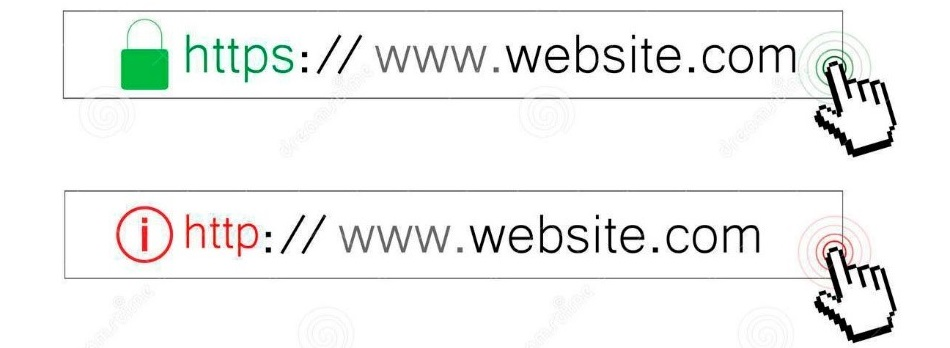
\includegraphics[width=0.75\linewidth]{images/protocolo-https-http} 

}

\caption{Protocolo https vs http.}\label{fig:unnamed-chunk-10}
\end{figure}

Si haces click en el candado, éste te mostrará que se trata de una conexión segura, así como el certificado, cookies y la configuración del sitio web.

IMPORTANTE: Tener el candado no garantiza que la web sea legítima. Ya que los certificados de cifrado seguro los emiten terceros y los ciberestafadores pueden hacerse igualmente con uno.

\hypertarget{compras-y-transacciones}{%
\section{Compras y transacciones}\label{compras-y-transacciones}}

Para comprar por Internet debes tomar cuantas más precauciones mejor para evitar cualquier tipo de fraude. Los factores a tener en cuenta son los siguientes:

\begin{itemize}
\item
  Evita sitios webs que no te inspiren confianza: Por ello solo debes compras a través de webs y aplicaciones oficiales.
\item
  Busca valoraciones y opiniones: Para ello dispones de las reseñas de Google maps, así como también de plataformas como \href{https://es.trustpilot.com/}{Trust Pilot}, \href{https://www.localguidesconnect.com/}{Local guides connect} o \href{https://www.tripadvisor.es/}{TripAdvisor}.
\item
  Utiliza plataformas que valoran la reputación online de un portal, como \href{https://www.scamadviser.com/}{Scamadviser}.
\item
  Usa solo plataformas con protocolo HTTPS: Visto en el apartado anterior.
\item
  Utiliza navegación privada: Así evitarás que se registre el historial de navegación.
\item
  Trata de usar pasarelas de pago: Evita en lo posible el uso de tarjetas de crédito y opta por una pasarela de pago, como puede ser \href{https://www.paypal.com/es/home}{PayPal}, te estarás garantizando la compra, además de disponer de protocolos de devolución del importe muy efectivos.
\item
  Haz comprobaciones adicionales:

  \begin{itemize}
  \item
    Comprueba que la web está adherida a alguna plataforma de confianza online, como, por ejemplo, \href{https://www.confianzaonline.es/}{Confianza Online}. Se trata del único sello de calidad que cuenta con los reconocimientos de la Comisión Europea, el Instituto Nacional de Consumo o la Agencia Española de Protección de datos, además de estar respaldado por el Ministerio de Industria, Energía y Turismo. Y acredita que se cumple con los estándares de privacidad y protección de datos de los usuarios entre otros. También existe el \href{https://www.aenor.com/certificacion/tecnologias-de-la-informacion/buenas-practicas-comercio-electronico}{Certificado de comercio electrónico} expedido por Aenor.
  \item
    Verifica que reciben análisis de seguridad periódicos realizados por plataformas como \href{https://www.mcafeesecure.com/certification}{McAfee Secure}.
  \item
    Asegúrate que disponen de certificados de autenticidad de la web y seguridad de las transacciones como los que ofrece \href{https://es.norton.com/internet-security}{Norton secured} o \href{https://www.comodo.com/home/internet-security/secure-shopping.php}{Comodo secure}.
  \item
    Estos sellos y certificados los encontrarás normalmente en la parte inferior de la web en forma de logos y debes hacer click en ellos para obtener más información sobre la entidad que los expide y la vigencia de éstos, ya que muchas webs fraudulentas utilizan sellos falsos.
  \item
    También tienes plugins como \href{https://chrome.google.com/webstore/detail/historial-de-precios/fdeopiliemdomncemeibjpmccgmnkfig?hl=es-419\&authuser=0}{Historial de precios} o \href{https://chrome.google.com/webstore/detail/alitools-shopping-assista/eenflijjbchafephdplkdmeenekabdfb?hl=es-419\&authuser=0}{Alitools shopping assistan} que verifican si el precio del producto o servicio que deseas adquirir ha sido inflando por algún tipo de campaña publicitaria, como es el caso del Black Friday en los que suelen subir los precios para justificar su descuento.
  \item
    Verifica que las reseñas sean legítimas con plataformas como \href{https://reviewmeta.com/}{Review Meta} y \href{https://www.fakespot.com/}{Fake Spot}. Si quieres saber más sobre las campañas de reseñas fraudulentas lee esta entrada sobre \href{https://www.genbeta.com/actualidad/asi-incentivaban-a-crear-resenas-falsas-proveedores-chinos-baneados-amazon}{reseñas falsas}.
  \end{itemize}
\end{itemize}

\begin{figure}

{\centering 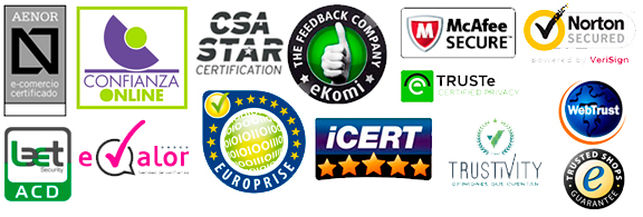
\includegraphics[width=0.75\linewidth]{images/sellos-de-confianza-online} 

}

\caption{Sellos y certificados de comercio online.}\label{fig:unnamed-chunk-11}
\end{figure}

Tienes disponible más información sobre compras online en \href{https://www.aepd.es/sites/default/files/2019-09/guia-compra-segura-digital-web.pdf}{Compra segura en internet (Guía práctica)} y también dispones de esta entrada de \href{https://www.osi.es/es/actualidad/blog/2018/08/08/detectando-fraudes-analisis-de-una-web-de-venta-falsa}{cómo detectar fraudes y análisis de una web falsa}.

\hypertarget{wi-fi}{%
\section{Wi-Fi}\label{wi-fi}}

Con respecto a la Wi-Fi nos encontramos ante dos escenarios: Wi-Fi propia y Wi-Fi ajena.

Uno de los peligros a los que más expuesto estás, es en el uso que haces de los puntos Wi-Fi ajenos. Ya que por lo general suelen ser puntos de accesos a la red gratuitos. En este escenario, existe el riesgo que aun tratándose de una red confiable puede haber sido hackeada por un tercero o que en primera instancia no provenga ni si quiera de una red de confianza. En cualquiera de los dos supuestos, tus dispositivos quedan expuestos y con ello, toda tu información sensible, a merced de ser espiado, robado o extorsionado.

Es por ello que debes tener la precaución de no hacer transacciones de ningún tipo, ni enviar datos sensibles. Es decir, usarla solo en caso de no te quede otra opción o en caso de tener que hacer cualquier búsqueda de carácter trivial.

Es de suponer que si estas en casa con Wi-Fi propia, estas recomendaciones no son tan necesarias. Pero si que sería muy recomendable por tu parte, que tuvieses muy en cuenta las recomendaciones que tienes a tu disposición en el apartado de Router en este manual. Además es conveniente que si no has establecido las capas de seguridad que se recomiendan en ese apartado, hagas una revisión de tu conexión Wi-Fi, por si tienes algún intruso y de ser así poder eliminarlo. Para ello tienes a tu disposición en el \href{https://www.osi.es/es/actualidad/blog}{blog de la Oficina de Seguridad de Internauta} un recurso llamado \href{https://www.osi.es/es/actualidad/blog/2019/09/25/descubre-y-elimina-los-intrusos-de-tu-red-wifi}{descubre y elimina a los intrusos de tu red wifi}.

Lo más recomendable es que siempre que puedas navegues con cable en lugar de Wi-Fi.

\hypertarget{plugins-o-extensiones}{%
\section{Plugins o extensiones}\label{plugins-o-extensiones}}

En informática, un complemento o plug-in es una aplicación (o programa informático) que se relaciona con otra para agregarle una función nueva y generalmente muy específica. Esta aplicación adicional es ejecutada por la aplicación principal e interactúan por medio de la interfaz de programación de aplicaciones. Complemento y plug-in se diferencian en que los complementos son desarrollados por empresas reconocidas y tienen certificado de seguridad y los plug-in pueden ser desarrollados por cualquiera \citep{IONOS-plugin}.

Existen una infinidad de plug-in de diferente naturaleza y para multitud de propósitos. En esta ocasión nos vamos a centrar en los usados por los navegadores, un ejemplo de estos es el archiconocido \href{https://getadblock.com/}{adBlock}, cuya función es la eliminar esos molestos anuncios de algunos portales webs.

Estos pueden estar desarrollados por terceros con intenciones de controlar la información que manejamos en nuestro dispositivo. De ahí que deban proceder de fuentes fiables y que estén configurados para actualizaciones automáticas.

Cada navegador dispone de repositorio de plug-ins o extensiones, que pueden ser consultados y desde donde los puedes instalar y comprobar su fiabilidad, así como consultar las valoraciones.

\begin{figure}

{\centering 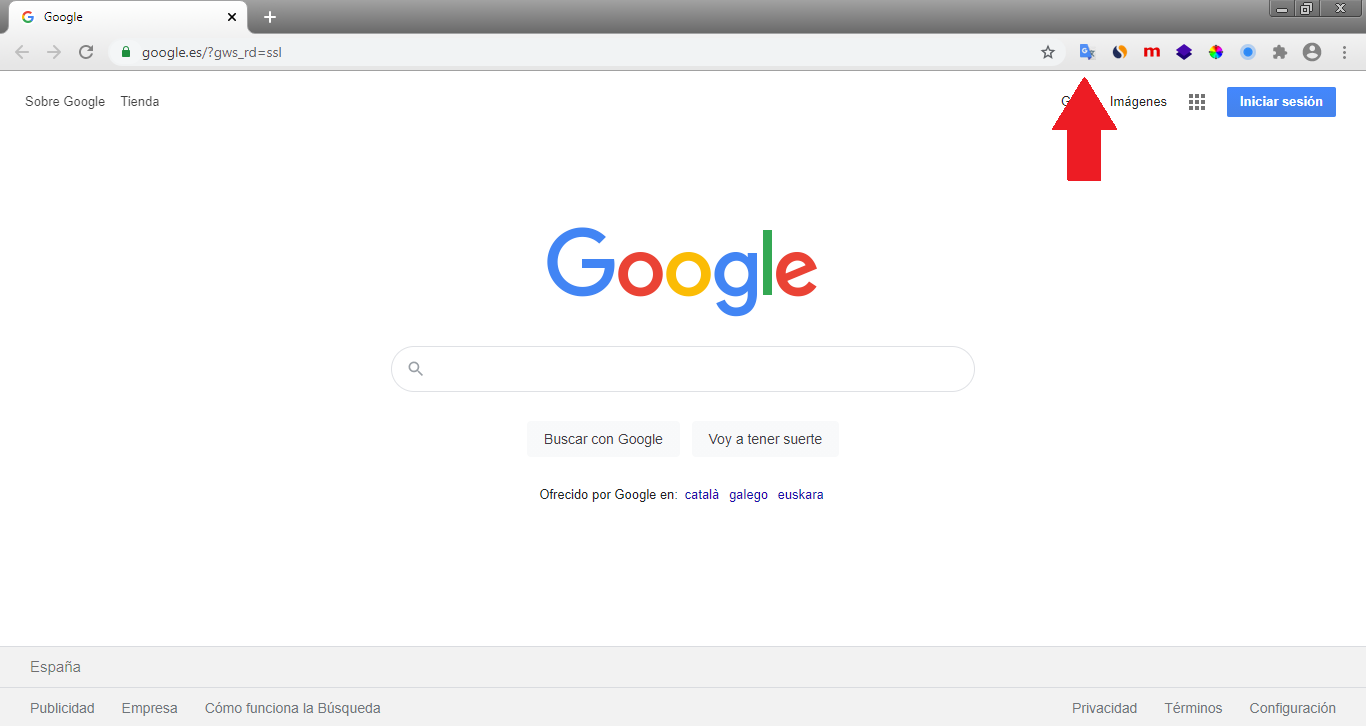
\includegraphics[width=0.75\linewidth]{images/plugin-navegador} 

}

\caption{Plugin traductor de Google seguido de otros plugin con diferentes funcionalidades.}\label{fig:unnamed-chunk-12}
\end{figure}

Si quieres ampliar tu conocimiento y saber más de plugins y extensiones pasate por el \href{https://www.osi.es/es/actualidad/blog}{blog de la Oficina de Seguridad de Internauta} y lee esta entrada sobre \href{https://www.osi.es/es/actualidad/blog/2019/11/20/extensiones-superpoderes-para-los-navegadores}{extensiones: Superpoderes para los navegadores}.

\hypertarget{descargas}{%
\section{Descargas}\label{descargas}}

Debes de tener muy en cuenta que las aplicaciones o programas deben ser descargadas desde sus sitios oficiales, y no desde otros. Es importante tener siempre presente que, incluso en ocasiones ni si quiera los antivirus reconocen algunas aplicaciones o programas que pudieran contener alguna vulnerabilidad, algún virus o gusano que afecte tu ordenador.

Existen también multitud de webs que en apariencia, ofrecen programas muy mediáticos o de mucha popularidad y que pueden haber sido previamente infectados con algún tipo de código malicioso mediante la modificación o alteración del mismo. Por ello, lo más aconsejable es que descarges las aplicaciones desde las webs oficiales \citep{software-alterado}.

Dentro de todos los tipos de archivos que pueden contener malware, uno de los más comunes es el .EXE. Incluso a la hora de descargar archivos de este tipo nuestro antivirus puede saltar aunque no se trate de una amenaza e incluso cuando quieras mandar un EXE por e-mail tampoco está permitido, por cuestiones de seguridad. Es todo un clásico, ya que se trata de un archivo ejecutable que podría instalar software malicioso en nuestro sistema. Hay que tener mucho ojo siempre que gestiones un archivo de este tipo \citep{RZ-exe}.

Es una buena práctica huir de portales de terceros, ya con los instaladores muchso de ellos descargan malware y molestas toolbars.

\hypertarget{cierre-de-sesiones}{%
\section{Cierre de sesiones}\label{cierre-de-sesiones}}

Cuando hagas uso de algún servicio en internet, como por ejemplo, Facebook, Gmail o cualquier otro, lo primero que tienes que hacer es iniciar sesión con tus credenciales.

Si estas en tu dispositivo no pasaría nada si una vez abierta la sesión no la cierras después de haber usado el servicio, pero si por el contrario estas usando un dispositivo ajeno, el servicio quedaría abierto y tus datos expuestos.

Por la razón antes expuesta, es importante que no dejes ninguna sesión abierta.

\hypertarget{sv-two-step-verification-o-verificaciuxf3n-en-dos-pasos}{%
\section{2SV (Two Step Verification) o Verificación en Dos Pasos}\label{sv-two-step-verification-o-verificaciuxf3n-en-dos-pasos}}

La mayoría de cuentas a día de hoy están configuradas para soportar lo que se conoce como SFA (Single Factor Authetication) o Factor de autenticación Simple. Se trata del acceso a cuentas o servicios con el solo uso del usuario y una contraseña, algo que todo el mundo viene haciendo desde hace tiempo. Esto se ha vuelto en gran medida un gran riesgo, ya que si un tercero consigue hacerse con tu contraseña no tendrá ninguna dificultad para tomar el control.

Es por este motivo que cada vez más servicios están implementando lo que se conoce como 2SV (Two Step Verification) o Verificación en Dos Pasos. Este sistema funciona de la siguiente manera, justo después de introducir tu contraseña, se te envía una notificación de forma segura al dispositivo en el que hayas iniciado sesión, de manera que solo tienes que aprobar la notificación para realizar el inicio sesión. Algunos servicios como la \href{https://support.google.com/accounts/answer/185839?co=GENIE.Platform\%3DDesktop\&hl=es}{verificación en dos pasos de google} viene de manera nativa y tan solo tienes que activarla.

Como puedes ver, los dos pasos son:

\begin{enumerate}
\def\labelenumi{\arabic{enumi}.}
\tightlist
\item
  Usuario y contraseña: Que solo tú conoces.
\item
  Notificación: Recibes un aviso en tu dispositivo.
\end{enumerate}

\begin{figure}

{\centering \includegraphics[width=0.75\linewidth]{images/verificación-dos-pasos} 

}

\caption{Verificación en dos pasos.}\label{fig:unnamed-chunk-13}
\end{figure}

Según la fuente que uses para informarte puede ser que termines sin comprenderlo del todo, ya que algunos medios también entienden la verificación en dos pasos (2SV) como un 2FA (segundo factor de autenticación). La diferencia es tan sutil que a veces es difícil de discernir, pero podría entenderse si ves el 2SV como una notificación que recibes y que apruebas sin más y la 2FA como un código que has de introducir. No obstante si quieres más información, en este enlace sobre \href{https://www.osi.es/es/actualidad/blog/2017/01/17/verificacion-en-dos-pasos-que-es-y-como-me-puede-ayudar}{verificación en dos pasos} encontrarás más detalles, además de enlaces hacia las distintas plataformas y redes sociales más populares para que puedas implementarlo.

Es extremadamente recomendable que uses este sistema de verificación en la medida que puedas. Recuerda que de un modo u otro la mayoría de servicios y plataformas disponen de esta capa de seguridad. Normalmente las encontrarás en Ajustes y Seguridad.

\hypertarget{mfa-multi-factor-authentication-o-autenticaciuxf3n-de-factores-muxfaltiples}{%
\section{MFA (Multi-Factor Authentication) o Autenticación de Factores Múltiples}\label{mfa-multi-factor-authentication-o-autenticaciuxf3n-de-factores-muxfaltiples}}

La autenticación de factor múltiple es una forma eficaz de aumentar la protección de las cuentas de usuario contra las amenazas más comunes, como los ataques de phishing, apropiación de cuentas, etc. Y se trata un método de control de acceso informático, en el que a un usuario, se le concede acceso al sistema solo después de que presente dos o más pruebas o factores diferentes de que es quien dice ser. Estas pruebas pueden ser diversas, como una contraseña, clave secundaria rotativa, un certificado digital instalado en el equipo, un token físico, etc. entre otros y son éstos lo que se conocen como factores de autenticación \citep{WIKI-multiple-factor}.

Son tres los tipos de factores de autenticación:

\begin{itemize}
\tightlist
\item
  Algo que sabes: Factor de conocimiento (contraseña, respuesta a una pregunta, un PIN).
\item
  Algo que tienes: Factor de posesión (tarjeta, smartphone, token hardware como las Security keys).
\item
  Algo que eres: Factor biométrico (huellas dactilares, escaneos de retina, reconocimiento facial, reconocimiento de voz o el comportamiento de un usuario).
\end{itemize}

\begin{figure}

{\centering 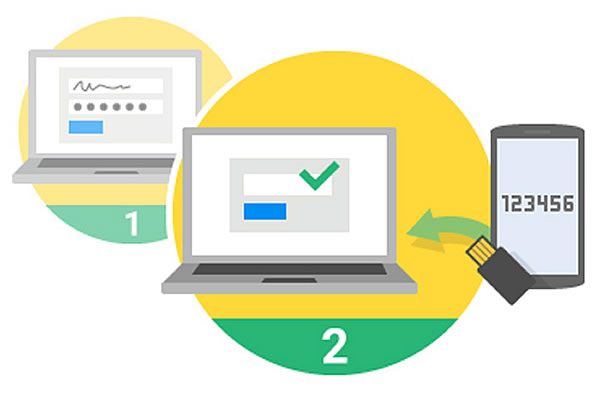
\includegraphics[width=0.5\linewidth]{images/autenticación-factor-múltiple} 

}

\caption{Autenticación de factores múltiples.}\label{fig:unnamed-chunk-14}
\end{figure}

Un de los ejemplo de autenticación en dos factores más común es la acción que realizas cuando vas a sacar dinero de un cajero. Por un lado metes la tarjeta (algo que tienes) y luego pones el PIN (algo que sabes). Esto es lo que se conoce como la autenticación en dos pasos o 2FA (segundo factor de autenticación) y que a veces tiende a confundirse con la verificación en dos pasos 2SV (Two Step Verification) que puedes verla en esta misma unidad.

Otro ejemplo son los inicios de sesión en los que se necesita un código adicional que es gestionado a través de correo electrónico, SMS o llamadas telefónicas, como es el caso de algunas entidades bancarias. Y en otros supuestos, aunque la plataforma disponga de dicho servicio necesitarás una aplicación externa como \href{https://support.google.com/accounts/answer/1066447?co=GENIE.Platform\%3DAndroid\&hl=es-419}{Google Autenticator} o \href{https://www.microsoft.com/es-es/account/authenticator}{Microsoft autenticator} entre otras y que se trata de una App de autenticación en dos pasos, que te genera el código adicional, que ha de ser utilizado inmediatamente ya que éste expira con el tiemplo.

También puedes hacer uso de autenticación de factores múltiples con lo que se conoce como Security Key o llave de seguridad. Se trata de un dispositivo hardware generalmente con conexión USB y necesitarás usar como segundo factor de autenticación una vez hayas introducido tu usuario y contraseña. En la publicación \href{https://es.digitaltrends.com/computadoras/las-mejores-llaves-de-seguridad-usb/}{las mejores llaves de seguridad usb} encontrarás algunos de los más utilizados y recuerda siempre comprar en las plaformas oficiales o de confianza.

En la mayoría de los casos solo se combinan dos de estos tres factores, aunque existe la posibilidad de implementar los tres si se viene necesario. Más información en \href{https://www.santander.com/es/stories/pon-una-capa-extra-de-seguridad-online-con-la-autenticacion-multifactor}{Banco Santander stories} y \href{https://protegermipc.net/2016/03/18/autenticacion-en-dos-factores-vs-autenticacion-en-dos-pasos/}{Autenticación en dos factores vs autenticación en dos pasos}

\hypertarget{cifrado-o-encriptaciuxf3n-de-datos}{%
\section{Cifrado o encriptación de datos}\label{cifrado-o-encriptaciuxf3n-de-datos}}

Tener datos o información simplemente organizados en carpetas en tus dispositivos sin más no es una práctica muy recomendable y más si se trata de datos sensibles. Para evitar que alguien que se haga con tu dispositivo pueda acceder impunemente a cualquier información es necesario disponer de una buena capa de seguridad. Es aquí donde entra en juego la herramienta de encriptado \href{https://cryptomator.org/}{Cryptomator}.

Cryptomator es un software libre y por lo tanto gratuito, con el que puedes encriptar tanto archivos como carpeta que quieras mantener a buen recaudo. Además es compatible con Windows, macOS y Linux y también disponen de una app para android y iphone.

Con Cryptomator puedes crear diferentes bóvedas o cámaras cifradas. Cada bóveda está protegida por una contraseña y puede contener tantos archivos y carpetas como desees. En estas bóvedas estará tu información encriptada de manera que no podrá ser visible a menos que poseas la contraseña que los desencripta. Con esta aplicación podrás estar tranquilo ya que nadie podrá acceder a tu información aun habiéndose hecho con tu dispositivo.

Otra interesante utilidad sería encriptar tus datos antes de subirlo a cualquier plataforma de almacenamiento en la nube con lo que te garantizas que no puedan ser leídos.

En la plataforma de \href{https://www.redeszone.net/tutoriales/seguridad/cryptomator-encriptar-archivos-carpetas/}{Redes zone} encontrarás más detalles de esta estupenda herramienta así como una guía para su instalación.

\hypertarget{antibotnet}{%
\section{AntiBotnet}\label{antibotnet}}

Un Botnet es el nombre genérico para denominar a cualquier grupo de PCs infectados y controlados por un ciberdelincuente de forma remota. Generalmente se trata de un hacker o un grupo de ellos los que crean el botnet a través de un malware que infecta a una gran cantidad de equipos. Este grupo de equipos o ordenadores son los que forman parte del botnet, o también llamados ``bots'' o ``zombies''. No existe un número mínimo de equipos para crear un botnet. Los botnets pequeños pueden incluir cientos de PCs infectados, mientras que los mayores utilizan millones de equipos \citep{INCI-botnet}.

Para saber si estás siendo víctima de este tipo de ataque, existen \href{https://www.osi.es/es/servicio-antibotnet}{servicios antibotnet} que identifican si desde tu conexión a internet se ha detectado algún incidente de seguridad relacionado u otras amenazas.

\hypertarget{bluetooth-y-nfc}{%
\section{Bluetooth y NFC}\label{bluetooth-y-nfc}}

El Bluetooth y NFC (Near field communication) o comunicación de campo cercano, son otro punto vulnerable en tu seguridad en la red. Pero antes veamos concretamente que son estos dos servicios.

\begin{itemize}
\item
  Bluetooth: Viene incorporado en multitud de dispositivos y permite conectarnos con otro dispositivo para compartir archivos o emparejar determinados dispositivos, como auriculares inalámbricos, etc \citep{IONOS-bluetooh}.
\item
  NFC: Se trata de una tecnología inalámbrica de corto alcance que permite conectar dos dispositivos entre sí para intercambiar información o realizar pagos \citep{IONOS-nfc}.
\end{itemize}

El riesgo que corres cuando tienes estos servicios activados es que el dispositivo de un tercero acabe sincronizándose con el tuyo, con el consiguiente riesgo que eso conlleva. Para evitarlo, una vez hayas terminado, mantenlos desactivados.

\hypertarget{amenazas}{%
\chapter{Amenazas}\label{amenazas}}

\hypertarget{principales-amenazas}{%
\section{Principales amenazas}\label{principales-amenazas}}

En lo referente a la seguridad de tus dispositivos debes tener en cuenta la diversidad de amenazas que existen, tales como virus, spywares, troyanos, gusanos y que pueden comprometer tus dispositivos y toda la información que en ellos contengas.

La mayoría de éstos están catalogado como Malware. Un Malware es un tipo de software malicioso con un primer objetivo inicial de infiltrarse en un equipo o sistema informático sin el consentimiento del usuario, para posteriormente actuar sobre él \citep{WIKI-malware}.

En este punto es importante que sepas cuáles son todas y cada una de las amenazas a las que estas expuesto, si no tienes las herramientas y no adoptas una actitud prudente en el uso de los dispositivos y la red.

En unidades anteriores viste que precauciones y herramientas debes adoptar para no correr riesgos. En esta unidad verás cuáles son estas amenazas y como llegan a tus dispositivos.

Las amenazas vienen de la mano de perfiles a los que conoces como hacker, ciberdelicuente, pirata informático, etc. Pero cabe destacar que estos conceptos no son lo mismo \citep{OSPI-ciberseguridad-espana}. Por lo tanto:

\begin{itemize}
\item
  Ciberdelincuentes: Sus ataques se dirigen a objetivos concretos como escuelas, hospitales, instituciones, grandes empresas o bancos, entre muchos otros.
\item
  Ciberterroristas y ciberyihadistas: Organizaciones terroristas que han desarrollado sus propias divisiones informáticas, aunque todavía no parecen ser capaces de desarrollar ciberataques sofisticados.
\item
  Hackivistas: Grupos reivindicativos que actúan por razones ideológicas.
\item
  Cibervándalos: Simplemente responden al deseo de armar revuelo y suelen ser ciberdelincuentes amateurs y poco cualificados.
\end{itemize}

Dispones de más información en \href{https://www.incibe.es/aprendeciberseguridad/hacker-vs-ciberdelincuente}{hacker vs ciberdelincuente} y \href{https://www.osi.es/es/campanas/los-ciberdelincuentes-quienes-son/quienes-son-los-ciberdelincuentes-y-que-buscan}{¿Quiénes son los ciberdelincuentes y qué buscan?}.

\textbf{¿Cómo detectar si estás infectado?}

\begin{itemize}
\item
  Cambios en el navegador, página de inicio distinta, nuevos favoritos o barras de herramientas.
\item
  Ordenador ralentizado.
\item
  Ventanas emergentes inesperadas.
\item
  Perdida de espacio en la memoría ram o disco duro.
\item
  Apagón del equipo de manera inesperada.
\item
  Mensajes anormales a la hora de encender el equipo.
\item
  Mensajes de alertas inesperados.
\item
  Ficheros cambiados de nombre o desaparecidos.
\end{itemize}

\textbf{Una buena práctica para minimizar los riesgos es disponer de una suite de seguridad que estaría básicamente formada por:}

\begin{itemize}
\item
  Antivirus.
\item
  Anti-Spyware.
\item
  Firewall o corta fuegos.
\item
  Copia de seguridad.
\item
  Discos de arranque.
\item
  Anti-phishing. El phishing lo verás en esta misma unidad más adelante.
\end{itemize}

\textbf{Si hay menores en casa:}

\begin{itemize}
\item
  Control parental.
\item
  Filtro web que restringe el acceso a contenidos no apto para menores.
\end{itemize}

\textbf{Los tres ciberataques que encabezan el ranking son:}

\begin{enumerate}
\def\labelenumi{\arabic{enumi}.}
\item
  Fraude de ventas.
\item
  Vulnerabilidad de los equipos.
\item
  Infecciones por malware que pretenden borrar datos, alterar las funciones básicas del equipo, espiar y/o robar datos.
\end{enumerate}

\hypertarget{virus}{%
\section{Virus}\label{virus}}

Un virus es un programa informático diseñado para infectar archivos u ocasionar efectos molestos, destructivos e incluso irreparables en tu ordenador, dañando hardware, software y archivos \citep{PANDA-virus}.

Los virus tienen diferentes vías de entrada a tus equipos, como por ejemplo:

\begin{itemize}
\item
  Utilización de una memoria USB previamente infectada.
\item
  Descarga de contenidos mediante redes de compartición P2P, u otras fuentes poco fiables.
\item
  Apertura de algún fichero adjunto en un correo electrónico.
\item
  Visitar una web maliciosa o pulsar sobre alguna dirección acortada que se publican en redes sociales u otros medidos y que en realidad no sabes a qué páginas web te puede llevar.
\end{itemize}

\hypertarget{gusanos-informuxe1ticos}{%
\section{Gusanos informáticos}\label{gusanos-informuxe1ticos}}

Los gusanos son en realidad una subclase de virus, por lo que comparten características similares \citep{PANDA-gusano}.

El principal objetivo de los gusanos es propagarse y afectar al mayor número de dispositivos posible, colapsar los ordenadores y las redes informáticas e impidiendo así el trabajo a los usuarios.

A diferencia de un virus, un gusano no necesita realizar cambios en los archivos de programas, sino que se aloja en diferentes ubicaciones del ordenador, principalmente la memoria RAM, para seguidamente clonarse a sí mismo y usar tus contactos y otros recursos del dispositivo para auto enviarse, a través del correo electrónico o programas P2P entre otros. Por lo que tienen la capacidad de propagarse sin la ayuda de una persona.

Los gusanos tienen diferentes vías de entrada a los equipos, como, por ejemplo:

\begin{itemize}
\item
  Utilización de una memoria USB previamente infectada.
\item
  Descarga de contenidos mediante redes de compartición P2P u otras fuentes poco fiables.
\item
  Apertura de algún fichero adjunto en un correo electrónico.
\item
  Visitar una web maliciosa o pulsar sobre alguna dirección acortada que se publican en redes sociales u otros medidos y que en realidad no sabes a qué páginas web te puede llevar.
\end{itemize}

\hypertarget{troyanos}{%
\section{Troyanos}\label{troyanos}}

Un Troyano o también llamado Caballo de Troya es una clase de malware que normalmente se camufla como software legítimo. Los ciberladrones utilizan este software malicioso para acceder en tus equipos y una vez dentro campar a sus anchas \citep{KASPER-troyano}.

Uno de los más peligrosos son los Keylogger es un tipo de software o un dispositivo hardware específico que se encarga de registrar las pulsaciones que realizas a través de tu teclado. Posteriormente son guardadas en un fichero y remitido a través de la red a los ciberdelincuentes.

Pudiendo llegar también como virus o gusanos, una vez activados, los troyanos pueden permitir a los cibercriminales espiarte, robar tus datos confidenciales y obtener acceso por una puerta trasera a tu sistema.

Los métodos más comunes de infección de un troyano suelen ser:

\begin{itemize}
\item
  La descarga de programas piratas o \href{https://es.wikipedia.org/wiki/Cracking_(software)}{crackeados}.
\item
  Descarga de programas gratuitos desconocidos (juegos, salvapantallas y aplicaciones sencillas relacionadas con el entretenimiento).
\item
  Abrir archivos adjuntos infectados.
\item
  Abrir una imagen o cualquier otro tipo de archivo que sea en realidad un ejecutable con extensión modificada.
\item
  Visitar sitios web trampa, es decir, sitios en los que para poder ver los vídeos sea necesario descargar un códec que en realidad es el troyano.
\item
  Visitar una web maliciosa o pulsar sobre alguna dirección acortada que se publican en redes sociales u otros medidos y que en realidad no sabes a qué páginas web te puede llevar.
\item
  Descarga de contenidos mediante redes de compartición P2P u otras fuentes poco fiables.
\end{itemize}

Existen herramientas que analizan y limpian los troyanos que se esconden en tu dispositivo y a su vez previene futuros ataques troyanos. Una de estas herramientas es el \href{https://www.avast.com/c-trojan-remover-tool}{Trojan remover}.

\hypertarget{ransomware-o-programa-rescate}{%
\section{Ransomware o programa rescate}\label{ransomware-o-programa-rescate}}

El Programa rescate o ransomware, está dentro del conjunto de software malicioso que también se conoce como malware y que impiden utilizar el equipo mientras el usuario no pague una cierta cantidad de dinero. El virus bloquea o cifra la información o datos del equipo \citep{WIKI-ransomware}.

Para intimidar y engañar a las víctimas les hacen creer que han incurrido en algún tipo de actividad delictiva, como incitación al odio, terrorismo o pederastia, entre otros.

En la actualidad estos son unos de los ataques más virulentos. Según un estudio realizado por la compañía \href{https://www.pandasecurity.com/es/mediacenter/seguridad/2019-tsunami-del-ransomware/}{Panda Security} en el 2019 este delitito tuvo un incremento con respecto al año 2018 del 500\%. Y según un estudio del \href{https://www.ospi.es/es/}{Observatorio del Sector Público de Inetum} solo en 2018, el número de afectados por estos ataques fue de más de 1.000 millones en todo el planeta.

\begin{figure}

{\centering 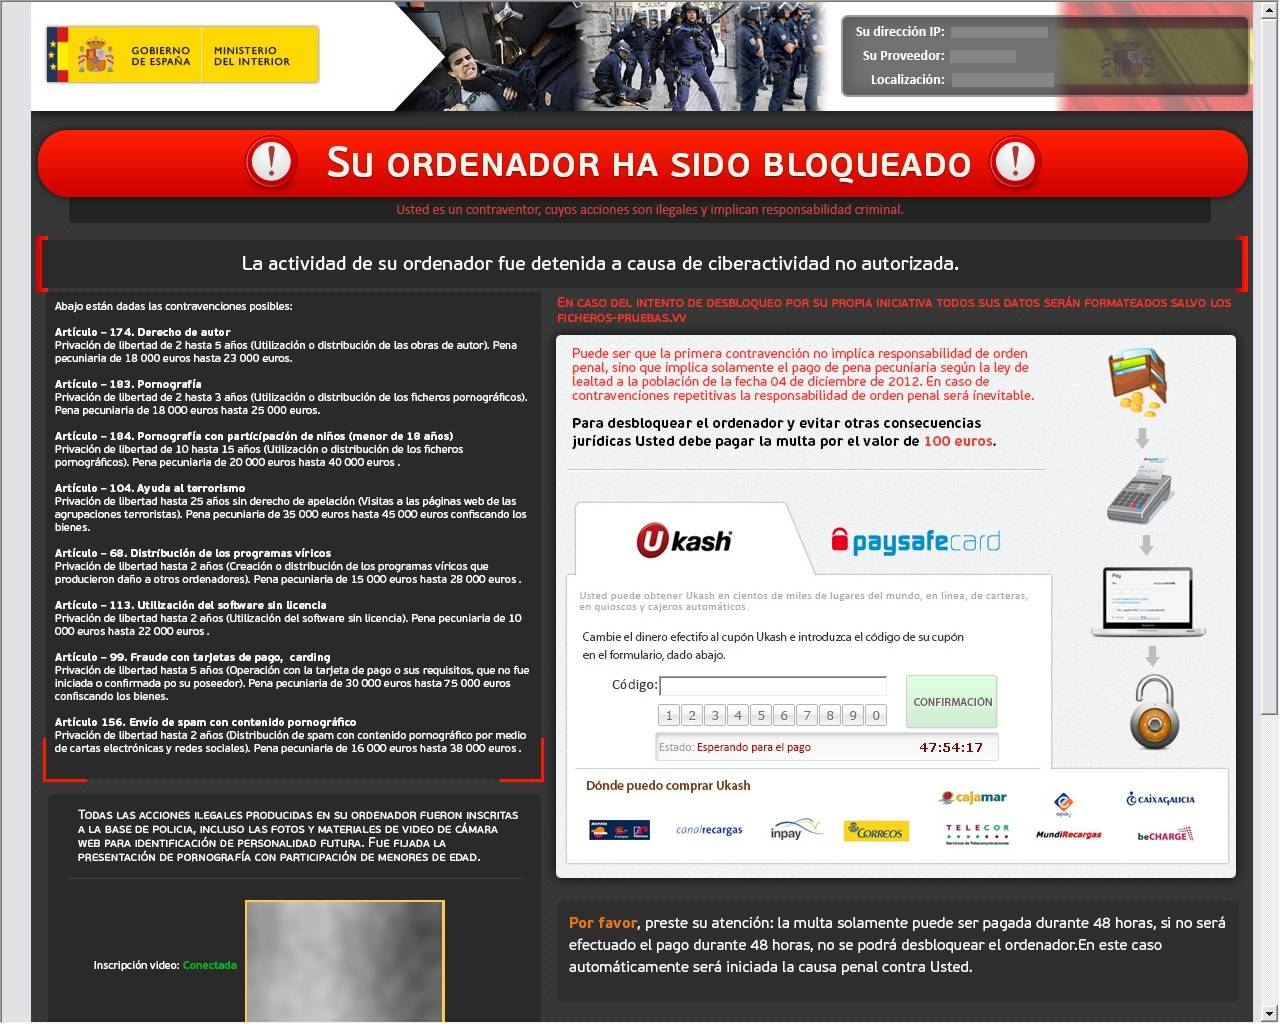
\includegraphics[width=0.75\linewidth]{images/ransomware} 

}

\caption{Ransomware (Malware).}\label{fig:unnamed-chunk-15}
\end{figure}

Las diferentes vías de entrada de ransomware a tu equipo son:

\begin{itemize}
\item
  Utilización de una memoria USB previamente infectada.
\item
  Descarga de contenidos mediante redes de compartición P2P, u otras fuentes poco fiables.
\item
  Apertura de algún fichero adjunto en un correo electrónico.
\item
  Visitar una web maliciosa o pulsar sobre alguna dirección acortada que se publican en redes sociales u otros medidos y que en realidad no sabes a qué páginas web te puede llevar.
\end{itemize}

En este punto cabe destacar que la firma de antivirus AVG pone a disposición del usuario una suite de herramientas gratuitas para \href{https://www.avg.com/es-es/ransomware-decryption-tools}{deshacer el cifrado del ransomware}, aunque quizá esto no siempre funcione.

Además en el caso del sistema operativo de Windows 10 en su última versión dispone de una protección de forma nativa contra ransomware, aunque esto no te garantiza estar inmunizado.

\hypertarget{spyware-o-software-espuxeda}{%
\section{Spyware o software espía}\label{spyware-o-software-espuxeda}}

El spyware es otro tipo de malware que se mantiene oculto mientras recopila información en secreto, que después transmite a una entidad externa, sin el conocimiento o el consentimiento del propietario del dispositivo \citep{AVAST-spyware}.

Puede supervisar y copiar todo lo que escribes, cargas, descargas y almacenas. Algunas cepas de spyware también son capaces de activar cámaras y micrófonos sin que te des cuenta.

Un spyware típico se auto instala en el sistema afectado de forma que se ejecuta cada vez que se pone en marcha el ordenador (utilizando CPU y memoria RAM, reduciendo la estabilidad del ordenador), y funciona todo el tiempo, controlando el uso que se hace de Internet e incluso algunos muestran anuncios no deseados.

Sin embargo, a diferencia de los virus, no se intenta replicar en otros ordenadores, por lo que funciona como un parásito.

El spyware tiene diferentes vías de entrada a los equipos, muy parecidas a los virus y gusanos:

\begin{itemize}
\item
  Descarga de contenidos mediante redes de compartición P2P u otras fuentes poco fiables.
\item
  Apertura de algún fichero adjunto en un correo electrónico.
\item
  Visitar una web maliciosa o pulsar sobre alguna dirección acortada que se publican en redes sociales u otros medidos y que en realidad no sabes a qué páginas web te puede llevar.
\end{itemize}

\hypertarget{adware}{%
\section{Adware}\label{adware}}

El Adware también un tipo de software malicioso que te muestra publicidad constante y molesta, bien instalando otro programa o con ventanas emergentes \citep{AVAST-adware}.

Las vías de entrada a son las mismas prácticamente que cualquier otro tipo de malware:

\begin{itemize}
\item
  Descarga de contenidos mediante redes de compartición P2P u otras fuentes poco fiables.
\item
  Apertura de algún fichero adjunto en un correo electrónico.
\item
  Visitar una web maliciosa o pulsar sobre alguna dirección acortada que se publican en redes sociales u otros medidos y que en realidad no sabes a qué páginas web te puede llevar.
\end{itemize}

Aunque parte de toda la molesta publicidad que recibes es legítima, existe una plataforma que se llama \href{https://www.listarobinson.es/}{Lista Robinson} a la que puedes inscribirte e indicar cuales son las empresas publicitarias de las que no quieres recibir publicidad y por qué medios no quieres recibir dicha publicidad: teléfono, correo postal, correo electrónico o SMS/MMS. Además se trata de un servicio gratuito.

Otro software muy útil contra la lucha de la publicidad no deseada es \href{https://www.ghostery.com/}{Ghostery} que se encarga de bloquear anuncios, detener rastreadores y acelerar sitios web. Ghostery descubre los rastreadores que hay tras cada sitio web y te permite controlar lo que no deseas para que tu experiencia de navegación sea más limpia, rápida y segura.

También es importante saber que prácticamente todos los medios sociales, como Facebook, Instagram, Google y demás disponen en sus menús de configuración de opciones para gestionar la publicidad que llega a tus dispositivos.

\hypertarget{malvertising}{%
\section{Malvertising}\label{malvertising}}

Malvertising es el acrónimo de las palabras Malicious y Advertising, que en español sería Publicidad Maliciosa. Esta amenaza lo que hace es esconder malware para infectar los dispositivos en los espacios de publicidad de otras páginas webs, como son los banner de publicidad en las cabeceras o laterales tanto izquierdos como derecho de muchas de la web que a diario te encuentras en internet.

La diferencia principal con el adware es que este primero necesita que el malware se instale en el dispositivo y en el caso del malvertising no es necesaria ninguna instalación por parte del usuario para resultar infectado \citep{OSI-malvertising}.

La vía de contagio por la que podemos caer víctimas de este ciberdelito, es como habrás podido ver, haciendo click en los anuncios en páginas webs.

\hypertarget{scareware-o-rogueware}{%
\section{Scareware o rogueware}\label{scareware-o-rogueware}}

Esta variante de malware conocido como Scareware o Rogueware es otro software malicioso más que trata de engañar a los usuarios para que visiten sitios infestados de malware. Normalmente suele darse en forma de ventanas emergentes, que además aparecen como advertencias legítimas de compañías de software en su mayoría de antivirus y que afirman que el sistema operativo ha sido vulnerado o que los archivos del PC han sido infectado \citep{KASPER-scareware}.

Las vías de contagio son las mismas que has visto en malwares anteriores:

\begin{itemize}
\item
  Descarga de contenidos mediante redes de compartición P2P u otras fuentes poco fiables.
\item
  Apertura de algún fichero adjunto en un correo electrónico.
\item
  Visitar una web maliciosa o pulsar sobre alguna dirección acortada que se publican en redes sociales u otros medidos y que en realidad no sabes a qué páginas web te puede llevar.
\end{itemize}

\hypertarget{malware-qr}{%
\section{Malware QR}\label{malware-qr}}

Los Quick Response (QR) son códigos de barra de dos dimensiones diseñados para ser leídos e interpretados rápidamente. Actualmente y sumado a la gran proliferación de smartphones en el mercado, son muy utilizados en publicidad y campañas de marketing. Esto es debido a su gran facilidad de manejo, ya que solo basta con apuntar con la cámara y el smartphone se encarga del resto.

Lamentablemente los códigos QR también pueden ser utilizados con fines maliciosos, de manera un ciberdelicuente podría usar el código QR para direccionar a los usuarios a páginas web phishing, descarga de malware o cualquier otra amenaza \citep{ESET-malware-qr}.

La vía de contagio como te habrás podido dar cuenta queda implícita.

\hypertarget{phishing}{%
\section{Phishing}\label{phishing}}

El término Phishing es utilizado para referirse a uno de los métodos más utilizados por delincuentes cibernéticos para estafar y obtener información confidencial de forma fraudulenta como puede ser una contraseña o información detallada sobre tarjetas de crédito u otra información bancaria de la víctima \citep{INFOSPY-phishing}.

El estafador, conocido como phisher, se vale de técnicas de \href{https://es.wikipedia.org/wiki/Ingeniería_social_(seguridad_informática)}{ingeniería social}, haciéndose pasar por una persona o empresa de confianza en lo que se conoce como suplantación de identidad o spoofing (término que verás más adelante en esta misma unidad) a través de una aparente comunicación oficial, por lo general un correo electrónico, redes sociales, SMS, etc., a raíz de un malware o incluso utilizando también llamadas telefónicas.

Los medios de phishing más usados por lo ciberdelincuentes:

\begin{itemize}
\item
  Correos electrónicos de carácter corporativo.
\item
  Mensajería instantánea.
\item
  Redes sociales.
\item
  Webs corporativas (Bancos, pasarelas de pago, tiendas online, etc.)
\item
  SMS.
\end{itemize}

Para poder detectar si estas siendo víctima de uno de estos fraudes debes estar atento a lo siguiente:

\begin{itemize}
\item
  La dirección web o URL: Fíjate muy bien en la URL a la que te remite el enlace que te envían. Insistir en que hay que fijarse muy bien porque en algunas ocasiones las diferencias son inapreciables y se centran incluso en caracteres que se copian o se alteran (una l minúscula por una i mayúscula; un punto situado en un lugar poco visible y otras estrategias).
\item
  Ortografía: Forma en la que está redactado el mensaje. Los ciberatacantes en algunos casos no tienen tu misma nacionalidad ni hablan tu misma lengua y, en muchas ocasiones traducen los textos automáticamente y contienen faltas de ortografía, errores gramaticales o un tratamiento o forma de dirigirse a ti que ninguna comunicación oficial de tu banco, organismos o empresas contendría.
\item
  Cuidado con el remitente y lo que solicitan: Correo electrónico de tu banco, de la Agencia Tributaria, de Amazon u otra empresa. Lo primero que debes mirar es el remitente y comprobar que esa dirección es la que está vinculada a esos servicios. De la misma manera, si el correo te ha llegado a la carpeta de spam ya es un signo inequívoco de que el remitente es sospechoso. ¿Qué te piden en el correo? Ten muy presente que los bancos y las empresas u organismos no reclaman jamás que introduzcas tus datos personales o que los reingreses en una web para reactivar tu cuenta. No lo reclaman jamás.
\item
  Desconfía de los cupones promocionales y las encuestas: Esta modalidad de phishing ha sido una de las que más éxito ha tenido en los últimos años y ha afectado a todas las grandes marcas. Existen ejemplos de phishing a Mercadona, Ikea, a El Corte Inglés, a Zara, a Lidl\ldots{} Y todo a través de cupones promocionales en los que te prometen una compra o un vale descuento a cambio de que accedas a un enlace y rellenes tus datos personales.
\item
  Descarga archivos adjuntos: Salvo que hayas comprobado todos los pasos anteriores y estés completamente seguro de la identidad del remitente, así como del objeto del mensaje, no descargues documentos adjuntos sin antes pasarlos por un buen antivirus.
\item
  Usa el sentido común y desconfía siempre: Este consejo es válido para detectar el phishing o cualquier otra amenaza en Internet. ¿Quién va a regalar gafas Ray-Ban o a venderlas un 75\% por debajo de su precio?.
\end{itemize}

\begin{figure}

{\centering 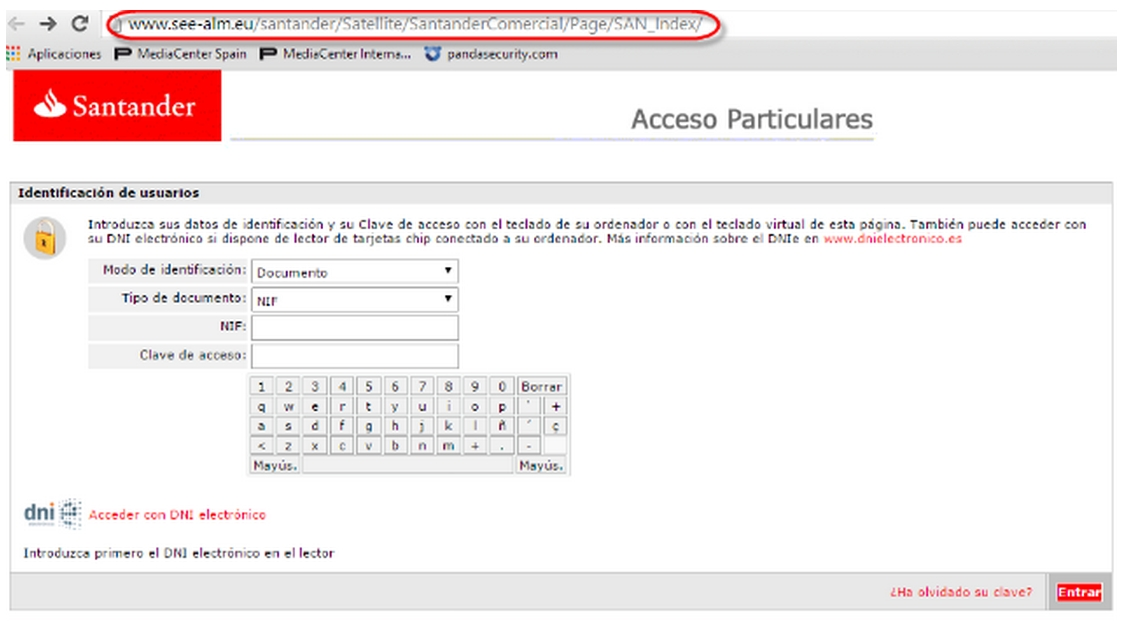
\includegraphics[width=0.75\linewidth]{images/phishing} 

}

\caption{Phishing banco Santander.}\label{fig:unnamed-chunk-16}
\end{figure}

En relación a la protección contra el phishing existen diferentes herramientas y servicios que puedes implementar en tu uso diario de las tecnologías. Algunos de estos son:

\begin{itemize}
\item
  Software anti-phishing: Software especifico para la detección de phishing.

  \begin{itemize}
  \item
    \href{https://home.sophos.com/es-es.aspx}{Sophos home}.
  \item
    \href{https://www.phishprotection.com/}{Phishing protection}
  \end{itemize}
\item
  Proveedores de email: Estos ofrecen protección contra el phishing a través de filtros y configuraciones con el objetivo detectar y frenar este tipo de fraude llevado a cabo por medio del correo electrónico. Para ello analizan de forma automatizada todos los emails, con el fin detectar links fraudulentos o dominios falsificados que tienen la intención de robar tus datos, protegiendo así a los usuarios de estos tipos de fraudes o estafas online. Esta protección puedes encontrarla prácticamente implementada en la mayoría de gestores de correos actuales.
\item
  Nativo del sistema operativo windows: \href{https://docs.microsoft.com/es-es/office365/servicedescriptions/office-365-advanced-threat-protection-service-description}{Anti-phishing defender}.
\item
  Antivirus: Algunos antivirus traen implementado estandares contra el phishing como el \href{https://support.eset.com/es/kb6380-activar-anti-phishing-en-productos-para-android-de-eset\#enable}{ESET anti-phising}.
\item
  Plugins: Extensiones para el navegador como lo es \href{https://www.zonealarm.com/es/anti-phishing/}{ZoneAlarm Web Secure Free}.
\item
  Código anti-phishing: Existen plataformas webs que ofrecen este servicio. Consiste en un código o palabra clave que tú facilitas la primera vez a la web y que esta incluye en sus futuros email, verificando así la legitimidad del mismo. Un ejemplo de ello lo econtrarás en la plataforma de intercambio de criptomonedas \href{https://academy.binance.com/es/articles/anti-phishing-code}{Binance código anti-phishing}.
\item
  Navegadores:

  \begin{itemize}
  \item
    \href{https://www.mozilla.org/es-ES/firefox/}{Firefox} es uno de los navegadores que implementan grandes capas de seguridad siendo una de ellas la protección anti-phishing y que además cuenta con \href{https://support.mozilla.org/es/}{Mozilla support} y \href{https://support.mozilla.org/es/kb/como-protegerse-del-phishing-y-del-malware-con-esta-herramienta-firefox}{Cómo protegerse del Phishing y del Malware con esta herramienta de Firefox}.
  \item
    \href{https://www.google.com/intl/es/chrome/}{Google Chrome} a su vez cuenta con los recursos ofrecidos por \href{https://safebrowsing.google.com/}{Google safe browsing}.
  \end{itemize}
\end{itemize}

Si quieres saber más sobre como evitar el phishing y de cómo saber identificar este tipo de fraude, visita el enlace de \href{https://www.osi.es/es/como-identificar-un-correo-electronico-malicioso}{Cómo identificar un correo electrónico malicioso}. Y además, si también quieres ver otros ejemplos de phishing de bancos como CaixaBank, Santander o BBVA, pasate por la siguiente publicación titulada \href{https://www.osi.es/es/actualidad/avisos/2021/06/detectadas-campanas-de-phishing-y-smishing-suplantando-diversas-entidades}{Detectadas campañas de phishing y smishing suplantando a diversas entidades bancarias} de la Oficina de Seguridad del Internauta, donde te encontrarás capturas de pantallas, detalles y soluciones que te ayudarán a salir airoso de este peligroso ciberdelito.

Otra técnica muy parecida al Phishing e igualmente peligrosa es el Pharming y que consiste en la explotación de una vulnerabilidad en el software de los servidores DNS (Domain Name System) o en el de los equipos de los propios usuarios, que permite a un atacante redirigir un nombre de dominio a otra máquina distinta. De esta forma, un usuario que introduzca un determinado nombre de dominio que haya sido redirigido, accederá en su explorador de internet a la página web que el atacante haya especificado para ese nombre de dominio \citep{KASPER-pharming}.

También existe otra amenza silimiar estas, conocida como Typosquatting, URL hijacking o fake URL. Está basada en los errores tipográficos cometidos por usuarios de internet cuando introducen la dirección de un sitio web en un navegador. Cuando esto sucede la dirección puede llevarlos a un sitio alternativo propiedad de un cybersquatter \citep{WIKI-typosquatting}.

\begin{itemize}
\tightlist
\item
  Ejemplo: \url{https://wikiepdia.org}
\end{itemize}

\hypertarget{vishing}{%
\section{Vishing}\label{vishing}}

El Vishing es una estafa que consiste en una llamada de teléfono en la que ciberdelicuente suplanta la identidad de una persona, empresa o institución para conseguir que le proporciones información privada y sensible. Esta información normalmente van a ser datos personales, contraseñas o peor aun los datos bancarios. Se trata de técnicas de ingeniería social con la que el estafador se va ganando la confianza de la víctima de manera que ésta termina proporcionandole cualquier tipo de datos. Si quieres saber más sobre ingeniería social visita este enlace \href{https://www.osi.es/es/actualidad/blog/2019/12/04/sabias-que-los-ataques-de-ingenieria-social-suponen-el-93-de-las-brechas}{¿Sabías que los ataques de ingeniería social suponen el 93\% de las brechas de seguridad?}.

En esta línea puedes encontrarte con lo que se conoce como pretexting o pretexto. Se trata en un ataque más de ingeniería social y que consiste en elaborar un
escenario o historia ficticia, donde el atacante tratará que la víctima comparta información que, en circunstancias normales, no revelaría. Habrás podido notar que a su vez también es la base del Phishing y del Smishing, que verás más adelante \citep{RZ-pretexting}.

Por lo tanto debes tener muy en cuenta, que cualquier petición de tus contraseñas o información financiera es una estafa, ya que las instituciones legítimas nunca te pedirían este tipo de datos tan sensibles a través del teléfono.

La vía de contagio como se ha señalado al principio es a través de una llamada de teléfono.

\hypertarget{smishing}{%
\section{Smishing}\label{smishing}}

El Smishing es un acrónimo formado por las palabras SMS y phishing, debido a su parecido con este ataque tan popular. La diferencia entre el Smishing y el Phishing, es que mientras este último lleva a cabo la estafa utilizando el correo electrónico como medio, en el Smishing se utilizan mensajes de texto enviados a través de SMS al smartphone o a través de las distintas aplicaciones de mensajería instantánea. Al igual que el phishing y el vishing, también se trata de una técnica de ingeniería social.

El modus operandi sigue siendo muy similar a otros ataques donde el ciberdelincuente suplanta la identidad de alguna persona o entidad de confianza de la víctima, con el objetivo de engañarla y conseguir que comparta información personal, realice un pago, haga clic en un enlace malicioso o se descargue un archivo adjunto entre otras.

El mayor riesgo de este tipo de ciberataque es el desconocimiento de los usuarios, ya que no esperan ser engañados a través de un mensaje de texto \citep{INCI-smishing}.

Como se ha destacado en líneas anteriores la vía de entrada de esta amenaza a través de SMS.

\hypertarget{spam-o-correo-malicioso}{%
\section{Spam o correo malicioso}\label{spam-o-correo-malicioso}}

Los términos spam o correo malicioso hacen referencia a los mensajes no solicitados, no deseados o con remitente no conocido (correo anónimo), habitualmente de tipo publicitario, generalmente son enviados en grandes cantidades (incluso masivas) que perjudican de alguna o varias maneras al receptor \citep{WIKI-spam}.

Su finalidad suele ser con motivos comerciales, pero también pueden contener enlaces peligros como el Phishing, solicitar datos sensibles o contener descargas que sean un riesgo para tu privacidad y seguridad:

\begin{itemize}
\item
  E-Mails Spam con fines comerciales
\item
  Envíos masivos / Avisos de virus
\item
  E-Mails con ofertas o regalos
\item
  Correos Phishing
\end{itemize}

Si recibes un email de carácter sospechoso, no lo abras y márcalo directamente como spam, para que así tu gestor de correos lo identifique para los sucesivos.

En este caso no hace falta destacar que este molesto malware llega por medio de gestores de correos.

\hypertarget{toolbars}{%
\section{Toolbars}\label{toolbars}}

Las Toolbars son barras de herramientas que aparecen en la parte superior de los navegadores. Generalmente sirven para tener enlaces más rápidos a servicios, por ejemplo Windows Live Toolbars da acceso al correo y búsqueda entre otras funcionalidades. Regularmente los navegadores tienen las suyas propias.

Pero puede ocurrir que a través de una instalación de software, normalmente gratuito puedan ser instaladas. Debes tener en cuenta que algunas de estas son muy molestas y en algunos casos pueden llegar a bombardearte con publicidad no deseada y que además en ocasiones llegan a ser muy difíciles de eliminar. Aunque cada vez son memos frecuentes.

\begin{figure}

{\centering 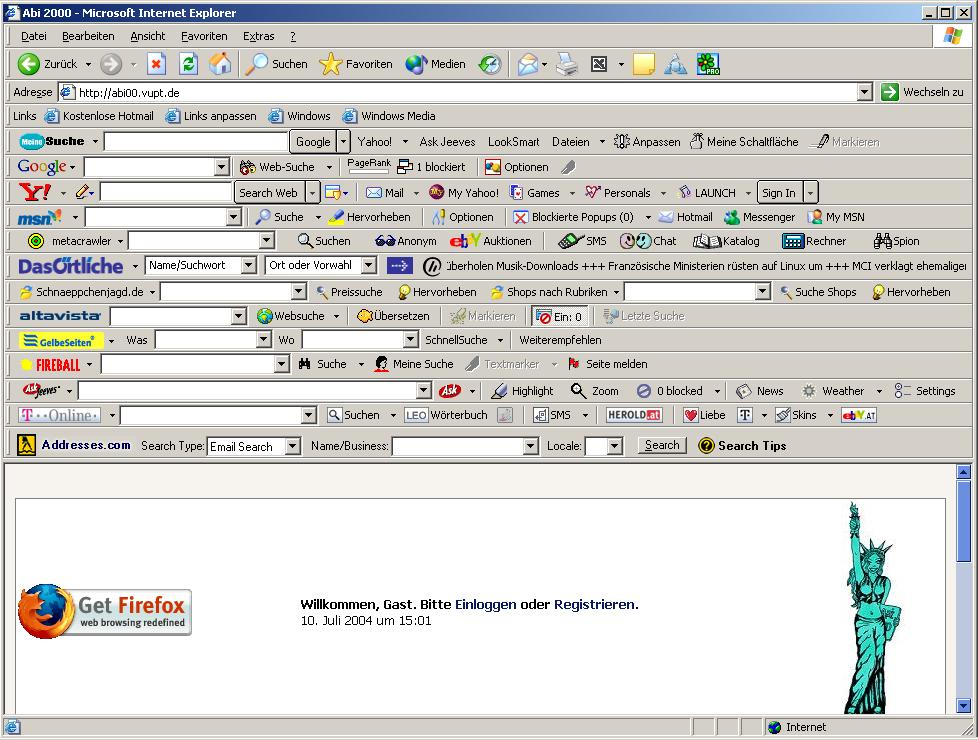
\includegraphics[width=0.75\linewidth]{images/toolbar} 

}

\caption{Toolbar.}\label{fig:unnamed-chunk-17}
\end{figure}

Normalmente, se instalan como un añadido al instalar aplicaciones gratuitas en el ordenador. Si no tienes cuidado durante el proceso de instalación y pulsamos siempre ``Siguiente-Siguiente-Siguiente'' las toolbars acaban en tu navegador. Para evitarlo no debes instalar una aplicación dando a ``Siguiente-Siguiente-Siguiente'' sin leer lo que nos están indicando. Para evitar este supuesto, recuerda que lo mejor es descargar programas solo de las webs oficiales.

En el caso de haber instalado alguna toolbars por descuido existen algunas herramientas para desinstalarlas fácilmente, entre ellas esta \href{https://es.malwarebytes.com/adwcleaner/}{Malwarebytes}.

Como se ha señalada más arriba la vía de contagio suele ser la instalación de software normalmente gratuito.

\hypertarget{usurpacion-o-robo-de-identidad}{%
\section{Usurpacion o robo de identidad}\label{usurpacion-o-robo-de-identidad}}

El robo de identidad, usurpación de identidad es la apropiación de la identidad de una persona: hacerse pasar por esa persona, asumir su identidad ante otras personas en público o en privado, en general para acceder a ciertos recursos o la obtención de créditos y otros beneficios en nombre de esa persona. Esto que sucede en el mundo analógico también ocurre en el mundo digital \citep{WIKI-usurpacion}.

La manera que tienen los ciberdelincuentes de usurpar la identidad suele ser a través de los siguientes:

\begin{itemize}
\item
  Robo masivo de cuentas de email por medio de métodos de hacking.
\item
  Por medio de Phishing, Smishing o Vishing.
\item
  Dejando tú cuenta abierta en sitios públicos.
\item
  Usando Wi-Fi de terceros creadas para ese fin.
\item
  Software espía o troyanos.
\end{itemize}

La usurpación de identidad permite a los delincuentes hacerse con información personal de sus víctimas, para luego con ella interceptar aún más datos de otros perfiles, a quienes engañan con el fin de extorsionar u obtener lucro económico e incluso a veces realizar actividades delictivas.
En caso de ser víctima de esta amenaza debes tener en cuenta lo siguiente:

\begin{itemize}
\item
  Guarda los mensajes de texto e emails que recibas.
\item
  Haz capturas de pantalla.
\item
  Revisa todas tus redes sociales.
\item
  Avisa a tus contactos sobre el perfil falso.
\item
  Infórmalo dentro de la aplicación. Todas las plataformas y redes sociales disponen de un apartado de Suplantación de indentidad en las cuentas.
\item
  Si es de carácter grave denúncialo a las autoridades.
\item
  Si es posible cancela cuenta.
\end{itemize}

En la \href{https://www.osi.es/es}{Oficina de seguridad del internauta} tienes una publicación que se llama \href{https://www.osi.es/es/actualidad/historias-reales/2021/03/05/me-han-secuestrado-mi-cuenta}{¡Me han secuestrado mi cuenta!} de una historia real donde puedes ver como gestionar este tipo de ataques.

\hypertarget{spoofing-o-suplantaciuxf3n-de-identidad}{%
\section{Spoofing o suplantación de identidad}\label{spoofing-o-suplantaciuxf3n-de-identidad}}

Normalmente cuando un ciberdelincuente usurpa un cuenta, ya sea particular o corporativa, la principal intención es hacer uso del spoofing o también conocido como suplantación de identidad. Estos términos pueden confundirse con el Phishing, pero no son lo mismo. Podría decirse que el Phishing es el término o palabra que se utiliza para describir la manera con la que los estafadores se hacen con tus datos y el spoofing son las herramientas, procedimientos o técnicas con los que lo lleva a cabo. Ejemplo: Un ciberestafador suplanta la web o el correo que recibes de tu entidad bancaria para que facilites tus datos, esta es la herramienta o herramientas y el término o nombre que recibe este acto es el Phishing. No obstante en el siguiente enlace puedes obtener más información sobre las \href{https://techlandia.com/diferencia-phishing-spoofing-info_241711/}{diferencias entre Phishing y Spoofing}.

A tener en cuenta también el hecho, que el uso de una acreditación física que no pertenece a su legítimo dueño, también esta considerado una estafa. Un claro ejemplo es el uso que hace un tercero de una tarjeta de identificación robada, para obtener el acceso a un determinado departamento físico de una compañía o empresa. Esto es lo que se conoce como \href{https://moodle2019-20.ua.es/moodle/pluginfile.php/113537/mod_resource/content/8/tema/4masquerading_mascarada.html\#:~:text=Consiste\%20en\%20suplantar\%20la\%20identidad,le\%20pertenecen\%20o\%20en\%20persona.}{Masquerating o suplantación de indentidad física}.

Otra actividad relacionada con la usurpación de identidad es el Brushing. Este delito es el que realizan algunos vendedores de Internet, que envían paquetes con objetos muy pequeños a diferentes usuarios para hacerse pasar por ellos y después poder valorar sus propios productos. Aunque en cierto modo esto no te pone en un serio riesgo, conviene conocerlo por si te sucede saber que se trata de una suplantación de la identidad y que es aconsejable interponer una denuncia \citep{brushing}.

\hypertarget{ciberestafas-en-compras-online-y-otros-engauxf1os}{%
\section{Ciberestafas en compras online y otros engaños}\label{ciberestafas-en-compras-online-y-otros-engauxf1os}}

Llegados hasta aquí, recordarte que todas las precauciones que se detallan en este manual en el apartado de Compras y transacciones de la unidad de Gestión de la seguridad en la red, son altamente recomendable en este punto. Además de ser fuertemente aconsegable seguir todas esas indicaciones, también se trata de tener en cuenta el conjunto de requisitos que veras a continuación, ya que cada uno de ellos por independiente te va a garantizar una capa más de seguridad y te irán indicando si puede o no puede ser una estafa.

Requisitos a comprobar:

\begin{itemize}
\item
  Formato seguro de URL: Https con su correspondiente candado. Aunque como has podido ver en el apartado de Protocolo https, los ciberdelincuentes también tienen acceso a este protocolo, por lo que no es seguro al 100\%.
\item
  Certificado de seguridad: Certifica que no ha sido vulnerada ni hackeada.
\item
  Sello de confianza y autenticidad: Verifican que se trata de una web legítima y confiable.
\item
  Conocer la empresa detrás de esa web, su ubicación, política de envío y de devolución, etc.
\item
  El precio que suele ser muy por debajo o simplemente con un descuento muy suculento.
\item
  Sorteos ganados bajo cualquier pretexto: Eres el visitante número 1.000 por ello te has ganado un premio.
\end{itemize}

Además puedes visitar la siguiente entrada donde aprenderás \href{https://www.osi.es/es/actualidad/blog/2018/08/08/detectando-fraudes-analisis-de-una-web-de-venta-falsa}{cómo detectar fraudes y análisis de una web falsa}.

Las estafas online no solo te las vas a encontrar en la compra de productos o servicios, sino que también en diferentes escenarios como los que verás a continuación. Pudiendo encontarlos a través de correos electrónicos, webs de venta de segunda mano, en webs maliciosas, etc.

Algunos ejemplos de estafas son:

\begin{itemize}
\item
  Timo Nigeriano: Lotería, viuda, enfermo terminal, herencias, etc.
\item
  Falsas ofertas de empleo: Ofertas de empleo bajo pago previo.
\item
  Falsos prestamistas de dinero: Que después de pagar los costes luego no recibes.
\item
  Novias rusas: Embaucan para posteriormente pedir dinero.
\item
  Falsos correos de sextorsión: Simulan que tienen fotos o vídeos comprometidos, cuando no es así.
\item
  Propuesta de compra del producto que tienes en venta: Solicitando que hagas el pago del envío por adelantado.
\item
  Pedir que hagas el pago o contactar contigo fuera de la plataforma de venta.
\item
  Otras muchas y nuevas que van ingeniando.
\end{itemize}

Las vías de entrada de las ciberestafas suelen llegar por medio:

\begin{itemize}
\item
  Correos electrónicos o mensajería instantánea.
\item
  Plataformas de venta de segunda mano.
\item
  Web de venta fraudulentas.
\item
  Redes sociales.
\end{itemize}

En esta \href{https://www.osi.es/es/guia-fraudes-online}{Guía de fraudes online} tienes un amplio catálogo de recursos para detectar si estas siendo víctima de una estafa o fraude online.

Por último, pero no por ello menos importante, si en algún momento te encontrases ante una posible estafa debes reportarlo a través desde este enlace para \href{https://www.incibe.es/protege-tu-empresa/reporte-fraude}{reportar webs fraudulenta en el Incibe}.

\hypertarget{vulnerabilidades}{%
\section{Vulnerabilidades}\label{vulnerabilidades}}

Una vulnerabilidad en términos de informática es una debilidad o fallo en un sistema de información, que pone en riesgo la seguridad de la información pudiendo permitir que un atacante pueda comprometer la integridad, disponibilidad o confidencialidad de la misma. Estas vulnerabilidades pueden tener distintos orígenes como por ejemplo: fallos de diseño, errores de configuración o carencias de procedimientos \citep{INCI-vulnerabilidad}.

Los fallos de vulnerabilidad les corresponde corregirlos a las terceras partes implicadas, lo a veces con lleva la dificultad de que escapan a nuestro control. Pero para protegernos de tales, debes tener actualizados todos tus sistemas y software.

Un ejemplo de vulnerabilidad muy conocido fuero el \href{https://es.wikipedia.org/wiki/Meltdown_(vulnerabilidad)}{Meltdown} y \href{https://es.wikipedia.org/wiki/Spectre_(vulnerabilidad)}{Spectre}, relacionadas con los procesadores informáticos, que existen desde mediados de los noventa, pero que han sido descubiertas ahora.

\hypertarget{cryptojacking}{%
\section{Cryptojacking}\label{cryptojacking}}

El cryptojacking, también llamado minería de criptomonedas malicioso, consiste en un tipo de software fraudulento que se oculta en un ordenador o en un dispositivo móvil, y utiliza los recursos de estos para extraer diversas formas de monedas digitales conocidas como \href{https://es.wikipedia.org/wiki/Criptomoneda}{criptomonedas}. Hay que aclarar que no está tan focalizado en el robo directo de estas, sino, que se centra en el robo o secuestro de dispositivos de terceros con el fin de utilizarlos para minar estas criptomonedas, y a los que se le conocen también como dispositivos zombies \citep{cryptojacking}.

Se trata de una amenaza reciente que se hace con el control del navegadores web, y de este modo, comprometen todo tipo de dispositivos, desde ordenadores de escritorio y portátiles hasta teléfonos inteligentes e incluso servidores de red.

Existen recursos y herramientas para saber si estamos siendo víctimas de cryptojacking \citep{GEN-guia-cryptojacking}:

\begin{itemize}
\item
  Te puede pasar que el ordenador se recaliente, que empiecen a sonar los ventiladores de pronto y se mantengan encendidos por más tiempo de lo que consideras normal.
\item
  El sistema operativo se pondrá lento, incluso se puede llegar a colgar el navegador o todo el sistema constantemente.
\item
  Comprueba el administrador de tareas en Windows, o el Monitor de actividad en MacOS. Fíjate en los procesos que estén ocupando el mayor porcentaje de CPU. En circunstancias normales un solo proceso no debe pasar de 10\%, rara vez sobrepasan el 20\% al menos que se trate de software muy complejo como el de edición de vídeo, juegos, o el mismo sistema actualizando. Pero que te aparezca el navegador en números absurdos como 70-90 y hasta 100\% es una alarma clara.
\end{itemize}

Las vías de contagios son las mismas que la mayoría de malware tales como los virus, gusanos, troyanos, spyware y demás. Por lo que puedes verlo en dichos apartados de esta misma unidad. Además existen webs y plugin que comprueban si estas siendo víctima de este ciberdelito e incluso alguna de estas herramientas previenen y bloquean estos ataques. A continuación tienes una lista para que puedas elegir la que mejor se adapte a tus necesidades:

\begin{itemize}
\item
  \href{https://github.com/fhstp/CoinEater}{CoinEater}
\item
  \href{https://github.com/xd4rker/MinerBlock}{Minerblock}
\item
  \href{https://notmining.es}{Not mining}
\item
  \href{https://github.com/keraf/NoCoin}{NoCoin}
\item
  \href{https://chrome.google.com/webstore/detail/nominer-block-coin-miners/jfnangjojcioomickmmnfmiadkfhcdmd}{NoMiner}
\item
  \href{https://github.com/hoshsadiq/adblock-nocoin-list}{Adblock nocoin list}
\end{itemize}

Señalar que \href{https://www.microsoft.com/es-es/windows/comprehensive-security}{Microsoft Defender}, que como ya sabréis es el antivirus que Windows trae por defecto ya incluye \href{https://www.microsoft.com/security/blog/2021/04/26/defending-against-cryptojacking-with-microsoft-defender-for-endpoint-and-intel-tdt/}{protección contra el cryptojacking}, aunque de momento solo está presente en la versión empresarial, es de suponer que con el paso del tiempo lo terminen incluyendo en las versiones de Windows Home.

\hypertarget{plugins-maliciosos}{%
\section{Plugins maliciosos}\label{plugins-maliciosos}}

En primer lugar, es importante tener claro qué es un plugin. Así pues, se trata de un software o aplicación que actúa como complemento para ampliar las funcionalidades del programa principal al que complementa. Dicho esto, algunos ciberdelicuentes usan esta funcionalidad para sus actividades delictivas, como espiar o recopilar datos sensibles e incluso el robo de criptomonedas. \citep{IONOS-plugin}.

Instalar un plugin suele ser una acción muy sencilla, y te puede servir para finalidades muy diversas, un claro ejemplo ello, es el plugin de \href{https://drive.googleblog.com/2012/12/introducing-save-to-drive-extension.html}{Google drive} o \href{https://getadblock.com/}{Adblock} para el bloqueo de publicidad, etc. Es por esto que debes tener siempre algunas consideraciones, como verás a continuación.

Sin embargo, a pesar de ser programas muy útiles que la inmensa mayoría utiliza, no todos son conscientes del riesgo que conlleva el simple hecho de instalar un plugin. El problema suele venir por no tener actualizado un buen sistema de seguridad.

A veces, el simple hecho de que el plugin este disponible no significa garantía ninguna. Tanto es así que aquí podemos ver uno de los que recientemente ha sido retirado de WordPress hasta en cuatro ocasiones. Un programa capaz de recopilar datos de los navegantes con el correspondiente riesgo a nivel de Reglamento General de Protección de Datos que esto conlleva, así como de publicar entradas no deseadas y prácticas de spam. De otra lado Google esta continuamente retirando plugins maliciosos de su plataforma.

El contagio de estos plugins maliciosos normalmente es a través de las Webs Store de las diferentes plataformas. Por lo que los puntos más importantes a tener en cuenta a la hora de protegernos son:

\begin{itemize}
\item
  Infórmate del desarrollo del plugin así como posibles variaciones.
\item
  No descarges plugins sospechosos.
\item
  Utiliza preferiblemente aquellos plugins de referencia, con fama y garantía reconocidas.
\end{itemize}

\hypertarget{sim-swaping}{%
\section{SIM Swaping}\label{sim-swaping}}

El SIM swapping, es la técnica que usan últimamente los ladrones digitales que se basa en duplicar la tarjeta SIM del móvil de sus víctimas. Así, pueden acceder a toda su información personal y, sobre todo, pueden usarlas en la verificación a través de un SMS por medio del móvil que suelen pedir los bancos cuando se opera a través de Internet y algunas otras plataformas online.

Por ello, aunque la mayoría de las apps de los bancos son muy seguras, con protocolos complejos para las claves de acceso, cifrado de las comunicaciones y teclados virtuales, los timadores digitales son capaces de saltarse la seguridad por medio de una técnica llamada \href{https://es.wikipedia.org/wiki/Ingeniería_social_(seguridad_informática)}{ingeniería social}, que consiste en el engaño a través de técnicas de persuasión y manipulación psicológica. Sin embargo, en lugar de timar directamente a las víctimas, el SIM swapping se consigue por medio de un engaño a los dependientes de las tiendas de telefonía.

Por lo tanto, una vez que el ciberdelicuente se hace con tus credenciales del tipo que sea, tales como contraseñas bancarias o de perfiles sociales, como Facebook, Instagram, etc o cualquier otra credencial privada, no va a tener problemas para obtener el SMS de verificación.

Cabe destacar que cuando se es víctima de este asalto digital, al obtener la duplicación de la SIM por parte del atacante, tu tarjeta queda sin uso, por lo tanto pierdes la cobertura de llamadas y la conexión de internet \citep{PANDA-sim}.

Por lo tanto, es importante que sigas estas recomendaciones para no ser víctimas del SIM Swapping:

\begin{itemize}
\item
  Utiliza una contraseña adicional o \href{https://www.osi.es/es/actualidad/blog/2019/02/27/el-factor-de-autenticacion-doble-y-multiple}{doble autentificación}: reconocimiento facial, por voz, PIN adicional, \href{https://play.google.com/store/apps/details?id=com.google.android.apps.authenticator2\&hl=es\&gl=US}{Google authenticator}, etc.
\item
  No compartas demasiada información en Internet. Cuantos más datos haya sobre ti en la web, más fácil será para los malos chantajearte, timarte o conseguir otras cosas tuyas, como contraseñas, cuentas bancarias, etc.
\item
  No almacenes todo en tu móvil, no es una caja fuerte. Es un dispositivo electrónico que no es 100\% seguro.
\item
  Exige a tu operador móvil que refuerce sus sistemas de seguridad cuando se trate de operaciones en tu nombre.
\item
  Los mensajes a través de aplicaciones de mensajería tipo WhatsApp, Telegram, Line, etc. son más seguros que los SMS, ya que están encriptados y éstos últimos no, haciéndolos más susceptibles.
\item
  No vincules tus cuentas bancarias a tu cuenta o teléfono.
\item
  No le des nunca a nadie tu código PIN. ¡Nunca!.
\item
  Instala un antivirus o solución de seguridad para evitar que puedan robar o acceder a tus datos personales.
\end{itemize}

Desde el \href{https://www.incibe.es/}{Instituto nacional de Ciberseguridad} y a través de este \href{https://www.youtube.com/watch?v=fIaodow_nxw}{video} podrás obtener más información sobre que es el SIM Swaping.

\hypertarget{shoulder-surfing-o-visual-hackins}{%
\section{Shoulder surfing o visual hackins}\label{shoulder-surfing-o-visual-hackins}}

El shoulder surfing o también conocido como visual hackins es una técnica en apariencia muy sencilla empleada por los ciberatacantes con el objetivo de conseguir información de un usuario en concreto. Esta técnica consiste en mirar literalmente por encima del hombro y que suele llevarse a cabo mientras viajamos en metro, en autobús o en cualquier sitio público donde los cibervándalos puedan estar atento al uso que haces de tu dispositivo sin que puedas percatarte de ello \citep{OSI-shoulder-surfing}.

Como has podido leer, evitar el uso de datos sensibles en espacios públicos es la mejor fórmula para evitar caer en este tipo de amenazas.

\hypertarget{ciberacoso}{%
\section{Ciberacoso}\label{ciberacoso}}

El ciberacoso es una forma de acoso o intimidación por medio de las tecnologías digitales. Su modus operandi se realiza en las redes sociales, las plataformas de mensajería, las plataformas de juegos, smartphones y cualquier otro dispositivo, plataforma o medio que disponga de conexión a internet. Es un comportamiento que se repite y que busca atemorizar, enfadar, humillar o maltratar a otras personas.

Ejemplos de ciberacoso son:

\begin{itemize}
\item
  Difundir mentiras o publicar fotografías vergonzosas de alguien en las redes sociales.
\item
  Enviar mensajes hirientes o amenazas a través de las plataformas de mensajería.
\item
  Hacerse pasar por otra persona y enviar mensajes agresivos en nombre de dicha persona.
\end{itemize}

El acoso cara a cara y el ciberacoso ocurren juntos a menudo. Pero el ciberacoso deja una huella digital, lo cual quiere decir, que queda un registro que puede servir de prueba para ayudar a detener el abuso \citep{ciberacoso}.

\hypertarget{ciberextorsiuxf3n}{%
\section{Ciberextorsión}\label{ciberextorsiuxf3n}}

La ciberextorsión es una forma de chantaje que sufre la víctima a través de los medios digitales, mediante el cual se le fuerza u obliga a pagar o a realizar algún acto o actividad delictiva o no lícita, para evitar los términos del chantaje. Un caso muy común es el del malware Ransomware que te obliga a pagar una cantidad de dinero si quieres recuperar tus archivos.

La plataforma de antivirus Panda Security pone a tu disposición una \href{https://www.pandasecurity.com/es/mediacenter/src/uploads/2016/02/Guia_Ciberextorsion-es.pdf}{Guía de ciberextorsión} para que puedas documentarte con más amplitud.

Dentro de la ciberextorsión se encuentra lo que se conoce como sextorsión. Este ciberdelito es también una forma de extorsión en el plano digital, pero en este caso con contenido sexual. En la sextorsión la víctima es amenazada con la supuesta publicación y difusión de contenido sexual.

\hypertarget{baiting}{%
\section{Baiting}\label{baiting}}

Para llevar a cabo el baiting los ciberdelincuente suelen utilizar dispositivos de almacenamiento extraíbles, normalmente memorias USB o incluso CDs y DVDs infectados con un software malicioso para posteriormente dejarlos en un lugar en el cual sea fácil de encontrar por la víctima como por ejemplo, baños públicos, ascensores, aceras, etc. Cuando la víctima encuentre dicho dispositivo y lo introduzca en su ordenador, el software malicioso se ejecutará de manera inadvertida y posibilitará que el hacker pueda acceder a los datos del usuario o usuaria \citep{baiting}.

La vía de contagio como te habrás podido dar cuenta queda implícita.

\hypertarget{clickjacking}{%
\section{Clickjacking}\label{clickjacking}}

El clickjacking busca usuarios desprevenidos que hagan clic en algún botón, pestaña o accedan a un enlace mientras navegan por internet, haciendoles creer que están ante algo legítimo y positivo para ellos. Suelen ser ganchos tales como, una oferta muy ventajosa o algo que provoque en la víctima la necesidad de entrar e informarse y de esta modo quedar infectado \citep{WIKI-clickjacking}.

\hypertarget{dumpster-diving-o-scavening}{%
\section{Dumpster diving o scavening}\label{dumpster-diving-o-scavening}}

Este ciberdelito se conoce como el proceso de buscar en tu basura para obtener información útil sobre ti o tu empresa que luego pueda ser utilizada en tu contra. Aunque este tipo de ataques esta más bien dirigido a empresas, debes tener cuidado con la información que desechas por el método de tirarlo a la basura. Nunca se sabe lo que los cibercacos están dispuestos a hacer \citep{WIKI-dumpster-diving}.

Cuando te deshagas del algún dispositivo físico de almacenamiento, ya sea un disco duro externo, un PC, un USB o cualquier otro dispositivo, asegúrate primero de eliminar totalmente todo el contenido. Para ello utiliza software de borrado definitivo, ya que un simple formateado no eliminará la información. El borrado solo se completa cuando se reescribe sobre la anterior información, es por esto que un formatero solo te hace constar que el espacio esta disponible, pero el contenido sigue estando ahí aunque oculto. Esto quiere decir que con software avanzado y específico los ciberdelincuentes podrían recuperar todo el contenido \citep{XATAKA-borrado-almacenamiento}.

Algunas herramientas de borrado definitivo son:

\begin{itemize}
\item
  \href{https://eraser.heidi.ie/}{Eraser}.
\item
  \href{https://www.diskwipe.org/download.php}{Disk wipe}.
\end{itemize}

Para evitar este tipo de amenaza ya sabes, ten cuidado con lo que tiras a la basura.

\hypertarget{quid-pro-quo}{%
\section{Quid pro quo}\label{quid-pro-quo}}

Según el diccionario de la lengua española el término ``quid pro quo'' es una locución latina que significa, cosa que sustituye a algo equivalente o que se recibe como compensación por ello. Sabiendo esto, el ciberdelincuente que emplea esta técnica, promete a su víctima un beneficio a cambio de información personal. Este beneficio suele ser compensaciones en formato regalo, como pueda ser merchandising, dinero, acceso gratuito a programas de pago, ayuda en servicio técnico, etc. Normalmente este ciberdelito te llegará a través de llamadas telefónicas o mensajes de supuestos expertos que ofrecen este tipo de compensaciones sin coste alguno \citep{quid-pro-quo}.

Las vías de contagio se han señalado más arriba y son las llamadas de teléfono o los mensajes con independencia de la naturaleza de estos.

\hypertarget{formjacking}{%
\section{Formjacking}\label{formjacking}}

El formjacking es la técnica que utilizan los ciberdelincuentes para interceptar la información que pones al comprar por Internet. Cuando entras en una página y realizas un pago, tienes que introducir los datos de tu tarjeta bancaria y esa es la información que busca el ciberestafador.

Esto lo llevan a cabo secuestrando los sitios webs donde habitualmente compran los usuarios. De esta forma la información que se introduce va a parar a un servidor controlado por ciberdelicuentes a través de lo que se conoce como la técnica de inyección de código malicioso, pudiendo así, robar información de pagos, número de la tarjeta o cualquier otro tipo de datos sensibles.

Es por ello que es muy recomendable evitar las páginas que puedan ser vistas como vulnerables, ya que éstas van a ser la vía de contagio. Aunque esto pueda parecer difícil de detectar, si ves una web con una estética un tanto antigua es posible que el resto de la web también este algo obsoleta y sea el objetivo de este ciberdelito \citep{RZ-formjacking}.

\hypertarget{juice-jacking}{%
\section{Juice jacking}\label{juice-jacking}}

Practicamente todo el mundo en algún momento se ha quedado sin carga en algunos de sus dispositivos, pero gracias a que existen multitud de cargadores de USB públicos, esto ya no es un problema. Pero detrás de los beneficios que esta práctica nos aporta, se esconde una amenaza que va proliferando cada vez más llamada juice jacking. El juice jacking consiste en alterar con fines maliciosos la fuente de carga de los USBs por parte de los diberdelincuentes y que a través de esta técnica pueden aprovecharse tanto para el robo datos como para la inyección de archivos \citep{ESET-juice-jacking}.

La vía de contagio de esta ciberamenaza queda evidente en lo anteriormente expuesto, por lo que intenta evitar en la medida de lo posible usar cargadores públicos.

\hypertarget{sustracciuxf3n-o-perdida-de-tu-dispositivo}{%
\section{Sustracción o perdida de tu dispositivo}\label{sustracciuxf3n-o-perdida-de-tu-dispositivo}}

Otra contingencia con la que te puedes encontrar es el robo o perdida de tu dispositivo. Si te encontrases ante esta posibilidad, a continuación tienes esta lista de todo lo que debes hacer para minimizar males mayores.

Qué hacer en caso de que hayas extraviado o te hayan robado tu dispositivo móvil:

\begin{itemize}
\item
  Pide a tu operadora que bloquee el IMEI de tu teléfono.
\item
  Búscalo con el localizador para \href{https://myaccount.google.com/intro/find-your-phone?hl=es-ES}{android} o para \href{https://www.apple.com/es/icloud/find-my/}{apple}.
\item
  Anula la SIM y pide duplicado de la misma.
\item
  Cambia todas tus contraseñas. ¡Todas!.
\item
  Denúncialo a la Policía.
\item
  Denúncialo a tu operadora
\item
  Avisa a tus contactos. Sí, a todos.
\item
  Bloquea el dispositivo y borra el contenido que puedas de forma remota.
\item
  Comprueba tu cuenta bancaria y ponte en contacto con tu banco.
\end{itemize}

Además de contar con los localizadores nativos de android y apple, en el siguiente enlace encontrarás otras apps para que puedas elegir la app que más te guste para \href{https://www.osi.es/es/herramientas-gratuitas?herramienta_selec\%5B0\%5D=122}{localizar tu dispositivo móvil}.

\hypertarget{tu-yo-digital}{%
\chapter{Tu yo digital}\label{tu-yo-digital}}

\hypertarget{toma-consciencia-de-tu-yo-digital}{%
\section{Toma consciencia de tu yo digital}\label{toma-consciencia-de-tu-yo-digital}}

En esta sociedad actual, tecnológica y digitalizada, de la que todos en mayor o menor medida formamos parte, debemos tener siempre presente que la forma en que desarrollamos nuestra personalidad, creamos nuestras relaciones sociales o gestionamos nuestra economía, nos lleva a definir nuestra imagen de marca y reputación digital.

En la esfera digital todas y cada una de nuestras acciones tendrá una repercusión directa en lo que el resto va a percibir sobre nosotros y por ende a definir quiénes somos, tanto desde una perspectiva personal, profesional como social creando constantemente y a veces casi de manera imperceptible nuestra identidad digital. Es por ello que no debes perder el foco y entender que esto va a contribuir y afectar a todas las capas de tu yo analógico.

Por lo tanto, en este nuevo escenario hacia la web 3.0 en la que ha aumentado la exposición a la superficie digital, y en el que el incremento exponencial de la ciberdelincuencia parece no tener freno, debes aprender y mejorar la experiencia digital y hacerla compatible con un uso responsable, respetuoso, crítico y creativo de la tecnología. Y a su vez desarrollar capacidades digitales que propicien un progreso inclusivo, seguro, privado y sostenibles que garantice el bienestar social.

\hypertarget{metadatos}{%
\section{Metadatos}\label{metadatos}}

Los metadatos pueden ser descritos de varias formas posibles, pero de forma resumida son un conjunto de datos que proporciona información de un recurso. Datos como pueden ser un archivo de imagen o un documento de texto, siendo algunos de éstos metadatos la fecha de creación, la de última modificación o la resolución en el caso de una imagen \citep{WIKI-meta}.

La función principal de los metadatos es la de ampliar con información adicional la contenida en el recurso del que forman parte con el fin de mejorar la calidad y efectividad de las búsquedas realizadas, no solo a la hora de realizar una búsqueda de un archivo perdido en nuestro sistema operativo, sino que esto afecta incluso al posicionamiento web.

En ciertas ocasiones éstos datos pueden provocar problemas, algunos de ellos de seguridad y privacidad como puede ocurrir por ejemplo por alguno de los dos motivos siguientes:

\begin{itemize}
\item
  Suele ocurrir que algunas cámaras fotográficas incluyan las coordenadas geográficas desde las que se realiza la fotografía entre los metadatos en los archivos de imágenes, pudiéndose localizar la posición en la que la imagen fue tomada. Esto es lo que se conoce como \href{https://es.wikipedia.org/wiki/Geoetiquetado}{Geoetiquetado}.
\item
  Puede determinarse la versión del software con la que fue guardado un archivo, por lo que si trabajas en una empresa y no tienes la licencia de dicho programa, los metadatos pueden generarte problemas.
\item
  La longitud de los mensajes, el autor, la localización, las fechas, la hora, etc. indentifican patrones de comportamientos, hábitos, relaciones y detalles personales. Todos estos datos son denominados el petróleo del siglo XXI \citep{OSI-petroleo-S-XXI}.
\end{itemize}

Para que puedas hacer una valoración de por que a todos los datos personales se les denominan el pretróleo del siglo XXI, visita la siguiente infografía de \href{https://www.osi.es/sites/default/files/images/concienciacion/c15-pdf-infografia-ciberdelincuentes_reyes.pdf}{cuál es el valor de tus datos en la red}.

\hypertarget{huella-digital-o-reputaciuxf3n-online}{%
\section{Huella digital o reputación online}\label{huella-digital-o-reputaciuxf3n-online}}

Eres lo que publicas, lo que compartes, con quién te relacionas e incluso lo que visitas desde tus dispositivos y todo este rastro es lo que compone la huella digital.

En otras palabras la huella digital o reputación online es la fama o prestigio que una persona o una empresa tiene en el mundo digital. Realmente la reputación digital no difiere mucho de la reputación tradicional, ya que en cierto modo ambas están conectadas, por lo que deben ser coherente la una con la otra.

Cabe destacar que la variante digital ha tomado gran importancia, ya que cuando una persona o compañía quiere saber de ti, uno de los mecanismos que va a utilizar es buscarte en internet, y es, en este punto donde radica la importancia de contar con una buena reputación online \citep{huella-digital}.

En este sentido es importante en un primer momento, conocer si tu huella digital goza de una buena salud y para ello lo más recomendable es que hagas un ejercicio de búsqueda, para ver si los resultados que obtienes son buenos. Puedes usar algunas de la siguientes herramientas para este propósito:

\begin{itemize}
\item
  Buscar directamente en google o otros buscadores. Puedes apoyarte en las \href{https://support.google.com/websearch/answer/2466433?hl=es}{búsquedas avanzadas de google}. Esto es lo que se conoce como Egosurfing.
\item
  También tienes plataformas que te ayudan a descubrir dónde están tus datos personales y poder gestionar tu huella digital. En los siguientes enlaces puedes encontrar dos de ellas \href{https://saymine.com/}{Say mine} y \href{https://www.jumboprivacy.com/}{Jumbo privacy}.
\item
  Crear alertas de \href{https://www.google.es/alerts}{Google alert}. Este rcurso también te servira para estar al día de lo que se publica sobre ti.
\item
  \href{https://www.hootsuite.com/}{Hootsuite}. Esta herramienta te buscará entre las principales redes sociales, como Facebook, twitter, etc. es usada en su mayoría en el mundo corporativo.
\end{itemize}

Si los resultados obtenidos no son de tu agrado, algunas plataformas te permiten solicita la eliminación de dicho contenido o simplemente puedes gestionar tú, esa información desde la propia plataforma. En el caso de Google puedes hacerlo a través de \href{https://myactivity.google.com/myactivity}{Mi Actividad}.

Crear una buena huella digital requiere de tiempo y debes ser cuidadoso con la manera en que interactuas en la red. Existen decálogos que te guían para crear una excelente reputación online, así como videos tutoriales y herramientas para llevarlo a cabo. Nos obstante aquí tienes las mejores recomendaciones para cuando quieras compartir, comentar, valorar o opinar en cualquiera de los medios sociales como Facebook, Instagram o cualquier otra, hacer una reseña en google o participar en algún foro \citep{decalogo-digital}.

\begin{itemize}
\item
  Presencia y actualización sistemática.
\item
  Cuidar la imagen mostrando transparencia.
\item
  Aportar contenido de calidad.
\item
  Respetar siempre la opinión ajena.
\item
  Identificar los canales apropiados con los que interactuar.
\item
  Tener en cuenta las reglas de urbanidad digital, esto consiste en una redacción cuidada y usos de negritas o enlaces de interés.
\item
  Diferenciar entre lo público y lo privado.
\end{itemize}

Estas últimas puedes tenerlas en cuenta si quieres llevar tu huella digital a un nivel más profesional.

\begin{itemize}
\item
  Disponer de un blog personal.
\item
  Mantener una actitud en la red activa.
\item
  Permanecer atento a las nuevas redes y formas de difusión.
\end{itemize}

\hypertarget{sombra-digital}{%
\section{Sombra digital}\label{sombra-digital}}

Cada foto que subes a Facebook, Instagram, cada mail que mandas, cada comentario o reseña que vas dejando en la web está generando lo ya conoces como huella digital. Hasta aquí todo bien, pero además de este rastro que es más o menos voluntario, también vas dejando otro rastro del que quizá no seas tan consciente, y a este rastro es al que se le conoce como sombra digital.

Ya en 2008 existían métricas que aseguran que la cantidad de información que se tiene de un individuo era mayor a la información creada por el mismo.

Partiendo de estos preceptos, la sombra digital es la información que queda de nosotros en los diferentes sistemas ya sean públicos o privados. Estos datos nos identifican y saben de nuestros gustos y preferencias. En la mayoría de los casos sin que nosotros mismos seamos conscientes de ello.

En este punto es cuando te estas preguntando como se crea la sombra digital. Pues bien, la sombra digital se va creando con el uso que haces de tus dispositivos, de la cámara en lugares públicos o privados, con el uso de la domótica como en el caso de las bombillas inteligentes y de otras múltiples maneras cuando interactuas con la tecnología. Los fabricantes introducen cookies y software especifico para este fin dentro de los sistemas operativos, para saber cuándo los usas, el tiempo que empleas, si usas hardware externo del tipo que sea e incluso para hacer un mapa de tu casa mientras usas tu aspiradora inteligente. Como verás la sombra digital se va construyendo por si sola.

Este concepto podría considerarse como una vulnerabilidad más de tu privacidad, pero también puede ser de mucha utilidad, como por ejemplo, cuando Google maps analiza tu movilidad para gestionar mejor tu trayecto, mostarte cuánto vas a tardar, que ruta puedes tomar y todo en tiempo real, algo que no sería posible sin la gestión de la sombra digital \citep{XATAKA-sombra-digital}.

\hypertarget{eliminar-el-historial-de-busquedas}{%
\section{Eliminar el historial de busquedas}\label{eliminar-el-historial-de-busquedas}}

Cualquier navegador, salvo que usemos una navegación privada, almacena un registro de las páginas que hemos visitado, una información que podemos borrar si queremos o conservar en el caso de querer localizar más tarde alguna página que no recordemos. Es muy útil en este segundo caso, pero puede llegar a ser embarazoso si no queremos que nadie pueda ver las webs que hemos visitado.

Cada navegador ofrece la posibilidad de borrar toda esta información y para ello puedes acceder desde los menús del propio navegador. Cada navegador tiene una forma diferente de realizar este borrado, aunque normalmente suele estar en la opción/pestaña herramientas. No obstante el siguiente enlace te llevará a la web del antivirus \href{https://www.avg.com/es/signal/how-to-clear-your-browsing-and-search-history}{AVG}, desde donde te enlazará a los diferentes tutoriales de cómo borrar el historial de navegación y de búsquedas de los navegadores más populares, como Google Chrome, Firefox o Microsoft Edge entre otros.

\hypertarget{derecho-al-olvido}{%
\section{Derecho al olvido}\label{derecho-al-olvido}}

El Reglamento General de Protección de Datos recoge una norma que permite a los usuarios poder ejercer su derecho al olvido. Esto quiere decir que todas las personas tienen el derecho de solicitar a los buscadores que eliminen todos los enlaces de datos personales que aparecen en sus resultados de búsqueda al introducir un nombre o cualquier otro dato personal. Dicho de otro modo, el derecho al olvido es aquel que tienen todos los ciudadanos a impedir la difusión de información personal a través de Internet.

Cabe aclarar que la eliminación de un enlace de un buscador no implica la desaparición de toda la información de carácter personal publicada en Internet. Este borrado sólo afecta a los motores de búsqueda que enlazan a dicho contenido \citep{OSI-derecho-al-olvido}.

Los siguientes enlaces te llevarán a los formularios de las plataformas detalladas donde podrás solicitar tu derecho al olvido:

-\href{https://support.google.com/websearch/troubleshooter/3111061?hl=es}{Solicitud de derecho al olvido de Google}

-\href{https://help.bing.microsoft.com/\#apex/18/ES/10013/-1/ES}{Solicitud de derecho al olvido de Bing}

-\href{https://es-us.ayuda.yahoo.com/kb/Eliminaci\%C3\%B3n-de-resultados-de-b\%C3\%BAsqueda-de-Yahoo-Search-sln4530.html}{Solicitud de derecho al olvido de Yahoo}

-\href{https://www.facebook.com/help/217091804975136}{Solicitud de derecho al olvido de Facebook}

Como podrás imaginar estas son las plataformas más relevantes, no obstante todas debe de tener esta opción. Si la plataforma a la que quieres solicitar tu derecho al olvido no esta entre éstas, solicítalo por el canal de comunicación que éstas tengan establecido.

Esto es parte de lo que se conoce como derecho al olvido. Si quieres más información visita el enlace \href{https://www.osi.es/es/actualidad/blog/2018/09/19/sabes-como-ejercer-el-derecho-al-olvido}{¿Sabes cómo ejercer el derecho al olvido?}.

\hypertarget{contenido-en-la-red}{%
\chapter{Contenido en la red}\label{contenido-en-la-red}}

\hypertarget{el-contenido-digital}{%
\section{El contenido digital}\label{el-contenido-digital}}

Cada vez más el contenido digital es mayor, a su vez va creciendo de manera exponencial y además esta disponible en multitud de formatos, como textos, imágenes, audio, vídeos. Llega a todos los públicos por diferentes canales y aún tratándose del mismo formato la manera en que el contenido esta mapeado o modelado, también es otra variante más de como la información llega al receptor final. Un ejemplo de como mapear o modelar una misma información en un mismo formato sería el uso de la representación visual o también conocido como Visual thinking y una infografía, ambos dos están representados en formato imagen.

La lectura que debes hacer en este punto, es que no toda la información vale y no todo el contenido es de calidad, por ello, tener claro los siguientes puntos pueden ser de mucha ayuda.

\hypertarget{constastar-la-informaciuxf3n}{%
\section{Constastar la información}\label{constastar-la-informaciuxf3n}}

Contrastar es sacar la información más relevante de los diferentes lugares en los que la encontramos, ya que se trata de una primera idea principal de aquello que necesitamos comprender o aplicar. Hoy en día la información en más rápida de encontrar y abundante en lo que se conoce como infoxicación. La \href{https://es.godaddy.com/blog/infoxicacion-causas-consecuencias/}{infoxicación} no es más que la sobrecarga de información a la que las personas se ven sometidas en su día a día, por lo que es importante saberla escoger, y saber que en muchos casos se trata de información irrelevante que algunas personas comparten simplemente por falta de conocimiento o criterio y en el peor de los casos para confundir.

Al contrastar información debes hacer un análisis de todas aquellas fuentes que encuentras, ya que los resultados de búsquedas en los navegadores es muy abundante y la información a veces es efímera y puede llegar a no estar totalmente actualizada, con lo que eso conlleva.

No debes conformarte con dar por buena la primera versión de una información en Internet, empobrece tu experiencia como usuario y te perjudica como lector. Por ello debes tener presente el compromiso ético, por mucho que las prisas sean las que mandes en algunas ocasiones, siempre debes cuidar tu ética al trabajar y contrastar muy bien toda información y fuente \citep{contrastar-informacion}.

\hypertarget{fake-news-y-deepfake}{%
\section{Fake news y Deepfake}\label{fake-news-y-deepfake}}

Las fake news son noticias sobre temas de interés social o de actualidad para crear una alarma o atraer la atención del mayor número de usuarios posibles y su objetivo principal es la desinformación. Suelen compartirse por redes sociales, correo electrónico o aplicaciones de mensajería instantánea como WhatsApp que aun contando con una \href{https://www.osi.es/es/actualidad/blog/2020/04/27/whatsapp-y-su-funcion-antibulos-descubrela}{función antibulos} no queda exenta \citep{OSI-bulos-buenas-practicas}.

Se diseñan y emiten con la intención deliberada de engañar, inducir a error, manipular decisiones personales, desprestigiar o enaltecer a una institución, entidad o persona u obtener ganancias económicas o rédito político, aunque en algunas ocasiones también incluyen promociones, ofertas y descuentos, especialmente en época de rebajas o compras navideñas \citep{WIKI-fake-news}.

De otro lado el deepfake es una técnica de inteligencia artificial que permite editar vídeos falsos de personas que aparentemente son reales, dando como resultado final un vídeo muy realista, aunque ficticio \citep{WIKI-deepfake}.

Amplia la información sobre deepfake en este artículo \href{https://computerhoy.com/reportajes/tecnologia/consiste-deepfake-446355}{¿Qué es y en qué consiste Deepfake?} de la revista digital Computer Hoy.

A continuación verás algunos consejos para poder hacer una buena criba de la información que te encuentes:

\begin{itemize}
\item
  Busca la fuente y contrasta la información.
\item
  Revisa la URL.
\item
  Mira más allá del simple titular.
\item
  Comprueba que el texto esta bien redactado.
\item
  Aplica el sentido común.
\end{itemize}

En esta entrada de Google llamada \href{https://blog.google/products/news/consejos-verificacion-hechos/}{Identifica la información falsa en línea con estos consejos} encontrarás más consejos para que detectar fake news te resulte más sencillo.

El compartir bulos o fake news aunque no seas consciente de ello fomenta la desinformación, en algunos casos la propagación de virus, malware o cualquier otra amenaza de las que ya conoces y además puede llegar a afectar negativamente a tu reputación digital, sin olvidarnos que afecta a tus contactos y a tu relación con ellos \citep{OSI-frena-evita-bulos}.

Cuando creas que te encuentras ante un posible bulo o fake news, ten en cuentas los siguientes:

\begin{itemize}
\item
  No los reenvíes.
\item
  No abras enlaces ni realices descargas.
\item
  Verifica la información.
\end{itemize}

En esta lista tienes plataformas que te ayudarán a identificar si estas ante una bulo o fake news:

\begin{itemize}
\item
  \href{https://toolbox.google.com/factcheck/explorer}{Google Fact Check Explorer}
\item
  \href{https://www.newtral.es/zona-verificacion/fact-check/}{Newtral}
\item
  \href{https://maldita.es/malditobulo/1}{Maldito bulo}
\end{itemize}

\hypertarget{deep-web}{%
\section{Deep web}\label{deep-web}}

El tema de la Deep Web es quizá un tema polémico y estigmatizado, pero al tratarse de una pieza más en este inmenso puzzle que es internet, es de recibo conocer al menos de que trata esto de la Web Profunda (Deep Web).

Existe una serie de contenido que por diversos motivos no está indexado en los buscadores convencionales como Google, Bing o Yahoo, entre otros y no siempre por temas de legalidad, moralidad o por no ser contenido lícito. Por ejemplo si estas en china y quieres acceder a Google no te va a quedar otro remedio que hacer uso de este servicio, ya que como sabrás China no permite el uso de Google, entre otros muchos servicios de internet. Es por esto y otras razones por lo que existe la Deep Web \citep{OSI-deep-web}.

De otro lado, esta el controvertido tema de las ilegalidades y otros asuntos turvios en lo que se conoce como la Dark Web y de los que no se va a tratar en este manual. Pero si quieres indagar por tu cuenta visita el siguiente enlace \href{https://www.xataka.com/analisis/una-semana-en-la-deep-web-esto-es-lo-que-me-he-encontrado}{Una semana en la Deep Web y esto es lo que me encontrado}.

\hypertarget{otras-particularidades-importantes}{%
\chapter{Otras particularidades importantes}\label{otras-particularidades-importantes}}

\hypertarget{otros-conceptos-relevantes}{%
\section{Otros conceptos relevantes}\label{otros-conceptos-relevantes}}

Existen otras muchas particularidades y conceptos que al no encajar de manera directa en unidades anteriores van a ser vistas en esta unidad. Aquí podrás ver otros aspectos relacionados con la privacidad y seguridad en internet que también te pueden ayudar a abordar todos estos temas.

\hypertarget{desinfecta-tu-dispositivo}{%
\section{Desinfecta tu dispositivo}\label{desinfecta-tu-dispositivo}}

Si crees que tu dispositivo puede estar infectado, aquí tienes una entrada de la Oficina de Seguridad de Internauta llamada \href{https://www.osi.es/es/desinfecta-tu-ordenador}{desinfecta tu dispositivo}, encabezada con los principales signos que pueden ponerte sobre aviso, así como las 3 fases de las que consta para solucionar este contratiempo y que son, una primera fase de primeros auxilios, una segunda fase de soluciones avanzadas y una tercera y última fase de solución definitiva.

\hypertarget{menores-en-el-uso-de-la-red}{%
\section{Menores en el uso de la red}\label{menores-en-el-uso-de-la-red}}

En lo que concierne a menores, la cuestión se torna más delicada, ya que se trata de grupo más inexperto y vulnerable, siendo 1 de cada 3 usuarios de internet un niño. En este manual no se va a tratar en profundidad este tema, ya que por si solo podría tratarse de otro manual completo, pero si cabe destacar algunos conceptos bastantes relevales como la educación, la concienciación y el seguimiento que tú, como padre, madre o tutor debes hacer del uso que hacen los menores de internet.

Por supuesto también has de conocer y hacerles saber de los peligros y amenzas con las que pueden encontrarse y que asechan tras la aparente inofensiva pantalla.

Sabes que entre el uso que hacen tus hijos de la red están actividades lúdicas como jugar, otras didácticas como aprender, otras sociales como relacionarse con amigos u otros y todo ésto, en la mayoría de la veces a tan solo solo click.

Pero no olvides que debes ser tú quien los guíe en la educación y concienciación, además de hacer un seguimiento de cerca para saber el uso que hace de las tecnologías. Para todo esto dispones de guías, herramientas, consejos, etc. Cabe destacar que es importante guiarlos para que tus menores hagan un uso responsable, respetuoso y de carácter prudente en el ámbito tecnológico, y que a su vez sean conscientes de todas las particularidades que conlleva interactuar tanto con los medios como con los dispositivos.

Por todo lo anteriormente expuesto, a continuación tienes estas sucintas listas como toma de contacto en lo que a menores se refiere.

Medidas con las que los menores deben comprometerse:

\begin{itemize}
\item
  No publicar fotos o vídeos de alguien sin permiso. (Válido también para adultos).
\item
  No usar la webcam con desconocidos. (Existen adesivos para taparla).
\item
  No creer en los regalos o chollos. (Ventanas pop-up - emails \ldots).
\item
  No aceptar amigos en la redes sociales que no conozcan. (No son amigos reales).
\item
  No ponerse en contacto con desconocidos.
\item
  No acordar citas con desconocidos a través de internet.
\item
  No facilitar datos personales. (Se sentirán más protegido/as).
\item
  No contestar a las provocaciones, ignóralas.
\item
  No hacer en la Red lo que no harían a la cara.
\item
  Tener cuidado con la información que comparten en línea. (incluyendo el correo, redes sociales como Instagram, TikTok\ldots).
\item
  Comportarse con educación en la Red.
\item
  Respetar los derechos de los demás en Internet. (No se debe reenviar material inadecuado por correo electrónico).
\item
  Si los molestan o amenazan, deben abandonar la conexión y pedir ayuda.
\item
  Mostrarse más celoso de su vida privada. (No diferencian bien entre público y privado, acostumbran a sociabilizar todos los aspectos de su vida).
\end{itemize}

Principales amenazas a la que los menores están expuestos:

\begin{itemize}
\item
  \href{https://ayudaenaccion.org/ong/blog/educacion/ciberbullying/}{Ciberbylling}.
\item
  \href{https://educacion2.com/que-es-el-fenomeno-gossip-e-informer/}{Gossip o informer}.
\item
  \href{https://www.aepap.org/sites/default/files/pags._131-142_ciberadicciones.pdf}{Ciberadicción}.
\item
  \href{https://www.educapeques.com/escuela-de-padres/vamping-definicion.html}{Vamping}.
\item
  \href{https://www.is4k.es/necesitas-saber/grooming}{Grooming}.
\item
  \href{https://www.is4k.es/menores-y-sexting}{Sexting}.
\item
  \href{https://www.levantalacabeza.es/obesidad-digital/}{Obesidad digital}.
\end{itemize}

Además conforme vayan creciendo se podrán ir topando con todos los peligros anteriormente vistos en este manual.

Qué debes enseñar a tus hijos como padre, madre o tutor:

\begin{itemize}
\item
  Concienciar a los menores sobre su actividad en la red. Aquello que salga de su móvil o correo no podrá recuperarlo jamás, perdurará en el tiempo y se trata de una información personal que cualquiera podría utilizarla.
\item
  Hacerles concientes de su identidad digital
\item
  Deben entender que navegar por Internet puede considerarse un derecho, pero también supone una responsabilidad. (Al igual que pasear por la calle no les da derecho a cruzar con un semáforo en rojo, navegar por Internet no les da derecho a entrar en un lugar que no deben).
\item
  Contraseñas seguras y diferentes. En la unidad de Gestión de la seguridad en la red de este manual encontrarás en el apartado de contraseñas todo lo que necesitas saber.
\item
  Es fácil deducir información personal de fotos o comentarios. (Lugar donde vive, los sitios que se frecuentas\ldots).
\item
  Enséñale a no hacer descargar programas sin tu permiso.(, música o archivos - propiedad intelectual, programas con virus, malware en naveradores\ldots).
\item
  Ayudar y enseñarles a protegerlos del spam. (Correos phising, software espia, malware\ldots).
\item
  Alertar a los menores que deben avisarles siempre que algún ``amigo de Internet'' insista respecto a informaciones o hábitos personales.
\item
  Deben saber que no están del todo seguro/a al otro lado de la pantalla.
\item
  El riesgo es el mismo en el mundo digital que en el real.
\item
  No toda la información en internet es veraz o fidedigna. (Contrastar varias fuentes).
\end{itemize}

Cuál es tu compromiso como padre, madre o tutor:

\begin{itemize}
\item
  Establecer espacios de trabajo independientes: es bueno que nuestros hijos tengan su propio espacio dentro del ordenador: su propio escritorio, su propio fondo de pantalla, su propia lista de favoritos, su propio sistema de carpetas. (De esa manera protegemos nuestros datos y les hacemos responsables de los suyos, pudiendoles crear un \href{https://securekids.es/que-es-el-control-parental-y-para-que-sirve/}{control parental} o restricciones mediante el navegador y apps para dispositivos móviles).
\item
  Establecer un horario de tiempo máximo de conexión.
\item
  Colocar el ordenador en una zona común.
\item
  Navegar por internet solo en presencia de un adulto. (Para que no crezcan como huerfanos digitales).
\item
  Estar informados del tipo y tiempo de navegación que hacen.
\item
  Manténganse actualizados con la tecnología. (No necesitas saber exactamente como funcionan todo, sólo necesitas saber qué son y para qué se usan. Ejemplo: no es lo mismo un chat que una app de mensajería instantánea.
\item
  Hablar habitualmente de las tecnologías y compartir actividad digital con ellos. (Respecto a la ``navegación'' que practican, a respetar las reglas y cumplir con obligaciones y acuerdos, a negociar y dialogar sobre los límites ``Reglas consensuadas'' para navegar en Internet).
\item
  Fomentar y premiar el uso adecuado y responsable de las tecnologías.
\item
  Disponer de antivirus.
\item
  Conocer el código PEGI (Pan European Game Information) que regula los juegos, donde se estipulan si con de carácter individual o colectivo, de estrategías, deportivos, shooting, aventura, etc.
\end{itemize}

Para ampliar la información dispones de dos exhaustivas guías de la Junta de andalucia \href{https://www.andaluciaesdigital.es/documents/20182/28716/Educar+para+Proteger+-+Guía+resumida+de+formación+TIC+para+padres+y+madres+de+niños+de+3+a+11+años.pdf}{Guía de formación TIC para padres y madres de menores de 3 a 11 años} y \href{https://www.juntadeandalucia.es/educacion/portalaverroes/documents/10306/1673096/Educar_para_proteger_Guia_Adolescentes.pdf}{Guía de formación TIC para adolescentes}.

Y en estos dos enlaces encontrarás dos prácticos recursos \href{https://families.google.com/familylink/}{Family Link by Google} y \href{https://securekids.es/}{Secure Kids}.

\hypertarget{utilidades-interesantes}{%
\section{Utilidades interesantes}\label{utilidades-interesantes}}

Aparte de todo lo visto en el manual existen muchas otras herramientas para ayudarte a salvaguardar tu privacidad y seguridad en internet, algunas de estas son:

\begin{itemize}
\item
  Correo electrónico (email):

  \begin{itemize}
  \item
    Emails temporales: Si solo necesitas regístrarte en una web para un recurso puntual, como por ejemplo descargarte un eBook, puedes utilizar \href{https://temp-mail.org/es/}{Temporay email} y no es el único servicio de este tipo, en siguiente enlace tienes una lista más amplia de \href{https://www.genbeta.com/correo/7-servicios-de-email-temporales-para-evitar-spam-y-otros-problemas}{servicios de correos temporales}. Y si usas el navegador Firefox, podrás tener este mismo servicio integrado en el propio navegador con solo la instalación del plugin \href{https://relay.firefox.com}{Relay firefox}.
  \item
    Emails anónimos: Con \href{https://www.secure-email.org/index.php}{Secure email} puedes enviar correos electrónicos y SMS anónimos, falsificar el número del remitente de SMS y muchos más.
  \item
    Modificar el alias o identidad del email: \href{https://simplelogin.io/}{Simple login} es un servicio con el que puedes crear tus alias o identidades para ocultar tu email personal, evitar spam y mantener tu privacidad.
  \end{itemize}
\item
  Escaneo de URLs maliciosas: \href{https://urlscan.io/}{UrlScan}. Esta plataforma detecta las direcciones webs fraudulentas.
\item
  Comprobar y mejorar tu privacidad y seguridad en internet: \href{https://securitycheckli.st/}{Lista de verificación de seguridad}. Esta web esta en inglés pero abarca un amplio espectro de herramientas y recursos diseñados para mejorar tu privacidad, seguridad y protección online y siempre dispones del traductor en línea de google.
\item
  Eliminar cuentas en Redes Sociales: \href{https://www.deseat.me/}{Deseat} es una plataforma con la que podrás tener instantáneamente una lista de todas tus cuentas y eliminar las que no estés usando o las que te apetezcan.
\item
  Números de teléfono de usar y tirar: \href{https://hushed.com}{Hushed} es un servicio premiun pero de coste muy económico. Solo es cuestión de ver si te compensa.
\item
  Nombres y direcciones desechables: \href{https://www.fakenamegenerator.com}{Generador de nombres falsos}. Como en el caso de los emails temporales este servicio puede ser un buen recurso.
\item
  Aviso de webs sospechosas: En el Chrome Web Store encontrarás este plugin que se llama \href{https://chrome.google.com/webstore/detail/suspicious-site-reporter/jknemblkbdhdcpllfgbfekkdciegfboi}{Suspicious Site Reporter} y que se encargará de avisarte si estas ante una webs de dudosa reputación.
\item
  Aviso de actividades sospechosas: Con \href{https://getlogdog.com/}{Get Logdog} recibirás alertas cada vez que ocurra una actividad sospechosa en tu Gmail, Facebook y otras cuentas.
\item
  Protección dispositivo móvil: \href{https://www.osi.es/es/conan-mobile}{Conan Mobile} te permite conocer el estado de seguridad de tu dispositivo, mostrándote soluciones a posibles riesgos a los que estés expuesto y proporcionándote algunos consejos que te ayudarán a mejorar su seguridad.
\item
  Verificadores de URLs acortadas: Comprobar la seguridad de una URL acortada antes de hacer click en ella es otra buena práctica para no acabar en una web de dudosa procedencia. A continuación tienes estos dos verificadores \href{https://unshorten.it/}{Unshorten} y \href{https://checkshorturl.com/}{Checkshorturl}.
\item
  Plugin o extensión antimalware: \href{https://www.mywot.com/}{MyWot} te mantendrá a salvo de estafas, malware, phishing y robo de identidad mientras navegas.
\item
  Centros de Seguridad:

  \begin{itemize}
  \item
    \href{https://safety.google}{Google}.
  \item
    \href{https://es-es.facebook.com/safety}{Facebook}.
  \item
    \href{https://about.instagram.com/es-la/community/safety}{Instagram}.
  \item
    \href{https://www.tiktok.com/safety?lang=es}{Tiktok}.
  \end{itemize}
\end{itemize}

\hypertarget{eventos-internacionales}{%
\section{Eventos internacionales}\label{eventos-internacionales}}

Durante el año, países e instituciones como la Comisión europea promueven iniciativas entorno al ecosistema tecnológico. Son organizadas a nivel internacional y donde pueden llegar a participar hasta más de 100 países. A continuación se muestras las de más repercusión mediática:

\begin{itemize}
\item
  \href{https://es.wikipedia.org/wiki/Día_de_Internet}{Día de Internet} (17 de mayo).
\item
  \href{https://es.wikipedia.org/wiki/Día_Internacional_de_Internet_Segura}{Día Internacional de Internet Segura} (Segundo martes de febrero).
\item
  \href{https://es.wikipedia.org/wiki/Día_mundial_de_la_contraseña}{Día mundial de la contraseña} (Primer jueves de mayo).
\end{itemize}

\hypertarget{colabora}{%
\section{Colabora}\label{colabora}}

Si eres una persona participativa y te gusta colaborar y aportar a los demás. Más abajo encontrarás una lista de actividades que podrás realizar, en las que no solo estarás ayudando a divulgar contenido y ayudar a otros, sino que además repercutirá de manera positiva en tu vida.

\begin{itemize}
\item
  \href{https://www.incibe.es/cibercooperantes/quiero-ser-cibercooperante}{Cibercooperante} (Incibe).
\item
  \href{https://www.cibervoluntarios.org/}{Cibervoluntario} (Ciber voluntarios).
\item
  \href{https://ayudaenaccion.org/ong/colabora/voluntariado-digital/}{Voluntario digital} (Ayuda en acción).
\item
  \href{https://twitter.com/Clicka_CRE}{Voluntariado digital} (Click\_A).
\end{itemize}

ANÍMATE!!! 😉

\hypertarget{formaciuxf3n-y-conocimientos}{%
\chapter{Formación y conocimientos}\label{formaciuxf3n-y-conocimientos}}

\hypertarget{aprendizaje-y-reciclado-continuo}{%
\section{Aprendizaje y reciclado continuo}\label{aprendizaje-y-reciclado-continuo}}

El aprendizaje y el reciclado continuo son dos de los pilares más importantes donde sustentar la educación. Por lo tanto sabrás que una buena educación abre puertas, facilita una mejor toma de decisiones y ayuda a evitar posibles escenarios futuros no deseados. Por lo tanto, es solo deber tuyo no descuidar la formación en conocimientos si quieres que sea tu mejor aliada para tu yo futuro y presente.

\hypertarget{formaciuxf3n-como-medida-preventiva}{%
\section{Formación como medida preventiva}\label{formaciuxf3n-como-medida-preventiva}}

En estos tiempos en los que de manera sutil nos vamos acercando a la cuarta revolución, marcada principalmente por la evolución de las tecnologías, la comunicación y la información entre otras. En los que estamos empezando a coquetear con los nuevos cambios de paradigma económico con la aparición de las criptomonedas, social con la multitud de plataformas y medios digitales de repercusión mediática y la descentralización con la nueva web 3.0, la tecnología Blockchain y el protocolo IPFS (InterPlanetary File System), solo nos puede llevar a pensar que no mantener una formación activa y estar actualizados, puede repercutir de manera desfavorable o negativa en la esfera social, profesional y personal en la que todos nos movemos.

Pon lo tanto, piensa que formarte para protegerte y sentirte seguro en el uso de las tecnologías es una inversión en bienestar y tranquilidad y que a mayor conocimiento, mayor protección y mejor gestión resolutiva.

En todo el grueso de esta manual tienes a tu disposición multitud de plataformas, recursos y herramientas con las que poder aprender y seguir instruyéndote en todo lo concerniente a privacidad y seguridad en internet, por lo tanto te animo a ir ampliando tus conocimientos cuando quieras y a tu propio ritmo. Porque ya sabes lo que dicen ``más vale prevenir que curar''.

No obstante si estas pensando dedicarte a esto de la ciberseguridad dentro del ámbito profesional, a continuación tienes un lista de formaciones más especificas y regladas.

\begin{itemize}
\item
  \href{https://learndigital.withgoogle.com/activate/course/cybersecurity-remote-work}{Ciberseguridad en el Teletrabajo}.
\item
  \href{https://www.cualifica2.es/cursos/Curso-Seguridad-En-Internet}{Seguridad en internet}.
\item
  \href{https://www.incibe.es/catalogos-formacion-ciberseguridad}{Catálogos de formación en ciberseguridad}.
\end{itemize}

\hypertarget{desarrolla-tu-ciberinteligencia}{%
\section{Desarrolla tu ciberinteligencia}\label{desarrolla-tu-ciberinteligencia}}

El término ciberinteligencia no es nuevo como tal, pero si que cada día cobra más vigencia y relevancia tanto en el mundo de los negocios como en el uso que hacen todos los usuarios del ciberespacio \citep{ciberinteligencia}.

Según el Centro de Tecnologías Emergentes de la \href{https://es.wikipedia.org/wiki/Universidad_Carnegie_Mellon}{Universidad Carnegie Mellon}, que es uno de los más destacados centros de investigación superior de los Estados Unidos en el área de ciencias de la computación y robótica, define la ciberinteligencia como:

``La adquisición y el análisis de información para identificar, rastrear y predecir las capacidades, intenciones y actividades cibernéticas que apoye la toma de decisiones''

Esta definición encaja muy bien en términos empresariales. Pero, ¿cómo prodría entenderse este concepto en el uso que hace el común de los mortales de internet?. Para responder a esta pregunta analicemos con más detalle la definición anterior. Si prestas atención verás que las pautas a seguir son:

\begin{itemize}
\item
  Adquisición de la información: Podría entenderse como los conocimientos adquiridos a través de la formación y el reciclado continuo.
\item
  Análisis: La formación adquirida provee de conocimientos para poder analizar el entorno donde mejor se mueven los ciberdelincuentes.
\item
  Predecir las capacidades, intenciones y actividades cibernéticas: Se entiende como la capacidad detectar posibles amenazas.
\item
  Toma de decisiones: Actuar en consecuencia para no llegar a ser una cibervíctima.
\end{itemize}

En definitiva la ciberinteligencia entendida desde el punto de vista de las personas podría entenderse como: Las competencias en conocimientos de las ciberamenazas existentes, la gestión de la privacidad y seguridad en los dispositivos y la red, apoyado en el uso de plataformas y software destinados a tal cometido. Siendo todo lo anterior lo que va a permir desarrollar las capacidades necesarias para la prevención, detección y reacción ante posibles ciberataques.

\hypertarget{pon-a-prueba-tus-conocimientos}{%
\section{Pon a prueba tus conocimientos}\label{pon-a-prueba-tus-conocimientos}}

Una manera de saber que conocimientos tienes sobre privacidad y seguridad en internet es poniéndote a prueba. Es por ello que a continuación tienes los siguientes recursos donde podrás calibrar cuanto sabes sobre tema. Porque recuerda, a mayor conocimiento, mayor protección.

\begin{itemize}
\item
  \href{https://www.osi.es/es/cuanto-sabes}{¿Cuánto sabes?}: Batería de cuestionarios de la Oficina de Seguridad del Internauta.
\item
  \href{https://phishingquiz.withgoogle.com/?hl=es}{¿Puedes detectar cuándo te están engañando?}: Prueba anti-phishing de Google.
\item
  \href{https://www.osi.es/es/campanas/ingenieria-social/prueba-deteccion-ingenieria-social\#collapsesuscripcion_index}{Prueba de detección de ingeniería social}: Test de la Oficina de Seguridad del Internauta.
\end{itemize}

\hypertarget{entidades-y-plataformas-de-ayuda}{%
\chapter{Entidades y plataformas de ayuda}\label{entidades-y-plataformas-de-ayuda}}

\hypertarget{ayuda-y-soporte-desde-instituciones}{%
\section{Ayuda y soporte desde instituciones}\label{ayuda-y-soporte-desde-instituciones}}

En internet existen multitud de plataformas y webs que te brindan la oportunidad de formarte y estar informado sobre ciberdelitos, ciberamenazas, privacidad y seguridad en internet y otro montón de conocimientos más. Además si sabes como abordar la plataforma verás que muchas de ellas son de autoridad reconocida. Aun así no deja de ser importante saber que desde nuestras instituciones existen proyectos específicos y gestionados por verdaderos expertos en la materia. Y es en esta unidad donde vas a ver con que entidades y plataformas puedes contar.

\hypertarget{instituto-nacional-de-ciberseguridad}{%
\section{Instituto nacional de ciberseguridad}\label{instituto-nacional-de-ciberseguridad}}

El Instituto Nacional de Ciberseguridad de España \href{https://www.incibe.es/}{INCIBE}, es una sociedad dependiente del Ministerio de Economía y Empresa a través de la Secretaría de Estado para el Avance Digital y consolidada como entidad de referencia para el desarrollo de la ciberseguridad y de la confianza digital de ciudadanos, red académica y de investigación, profesionales, empresas y especialmente para sectores estratégicos.

La misión de INCIBE es por tanto reforzar la ciberseguridad, la confianza y la protección de la información y privacidad en los servicios de la Sociedad de la Información, aportando valor a ciudadanos, empresas, Administración, red académica y de investigación española, sector de las tecnologías de la información y las comunicaciones y sectores estratégicos en general. Aunándolo es estas tres siguientes líneas de actuación:

\begin{itemize}
\item
  Al internauta.
\item
  Al menor.
\item
  A la empresa.
\end{itemize}

Informan entre otros sobre:

\begin{itemize}
\item
  Protección de redes, equipos y sistemas.
\item
  Cumplimiento de obligaciones relativas a la seguridad de la información.
\item
  Diferentes tipos de incidentes de seguridad.
\item
  Seguridad en las conexiones y redes wifi.
\item
  Configuración de la privacidad en dispositivos y servicios de internet.
\item
  Situaciones de infección por virus.
\item
  Contenidos inadecuados para menores y comunidades peligrosas en línea.
\item
  Ciberacoso escolar.
\item
  Controles parentales.
\end{itemize}

El Incibe tiene a disposición del ciudadano varios canales de comunicación:

\begin{itemize}
\item
  Teléfono gratuito \textbf{017}.
\item
  WhatsApp: \textbf{900 116 117}.
\item
  Telegram: \textbf{@INCIBE017}.
\item
  Formulario web: \textbf{\url{http://incibe.es/linea-de-ayuda-en-ciberseguridad\#formulario}}.
\end{itemize}

\hypertarget{oficina-de-seguridad-del-internauta}{%
\section{Oficina de seguridad del internauta}\label{oficina-de-seguridad-del-internauta}}

La Oficina de Seguridad del Internauta \href{https://www.osi.es/}{OSI} es una plataforma que proporciona información y soporte necesarios para evitar y resolver los problemas de seguridad a los que pueda enfrentarse el cuidadano en el uso de Internet.

El objetivo principal de esta entidad es reforzar la confianza en el ámbito digital a través de la formación en materia de ciberseguridad. Desde la Oficina de Seguridad del Internauta conjuntamente con el INCIBE trabajan para:

\begin{itemize}
\item
  Ayudar a los usuarios a llevar a cabo un cambio positivo de comportamiento en relación con la adopción de buenos hábitos de seguridad.
\item
  Hacerles conscientes de su propia responsabilidad en relación con la ciberseguridad.
\item
  Contribuir a minimizar el número y gravedad de incidencias de seguridad experimentadas por el usuario.
\item
  En este portal encontrarás información general sobre la seguridad en Internet y herramientas que te ayudarán a navegar más seguro.
\end{itemize}

Además de llevar a cabo todas estas líneas de actuación, a través de este portal también:

\begin{itemize}
\item
  Dispones de un \href{https://www.osi.es/es/actualidad/avisos}{canal de avisos} para estar actualizado de las últimas alertas de seguridad.
\item
  Podrás hacer \href{https://www.osi.es/es/reporte-de-fraude}{reportes de fraudes}.
\item
  En el menú de navegación encontrarás una pestaña de juegos educativos donde encontrarás recursos para aprender jugando, entre ellos toda una batería de \href{https://www.osi.es/es/juegos-mesa}{juegos de mesa}.
\item
  \href{https://www.osi.es/es/campanas}{Campañas de concienciación}.
\end{itemize}

Y esto no es todo, en esta plataforma encontrarás multitud de recursos y herramientas para gestionar o solventar cualquier incidencia en matería de privacidad y seguridad en internet.

\hypertarget{agencia-espauxf1ola-de-protecciuxf3n-de-datos}{%
\section{Agencia española de protección de datos}\label{agencia-espauxf1ola-de-protecciuxf3n-de-datos}}

La Agencia Española de Protección de Datos \href{https://www.aepd.es/es}{AEPD} es una entidad de ayuda a la ciudadanía más orientada a la privacidad en lo concerniente a tus datos personales. Actúan para proteger tus derechos de acceso, rectificación, limitación, oposición, supresión (derecho al olvido), portabilidad y oposición al tratamiento de decisiones automatizadas.

Entre los recursos que encontrarás en la plataforma están los siguientes:

\begin{itemize}
\item
  Derechos y deberes en el tratamiento de datos.
\item
  Ayuda a la ciudadanía.
\item
  Ayuda específica a menores.
\item
  Guías y herramientas.
\end{itemize}

\hypertarget{internet-segura-para-uxf1iuxf1os}{%
\section{Internet segura para ñiños}\label{internet-segura-para-uxf1iuxf1os}}

Internet Segura for Kids \href{https://www.is4k.es/}{IS4K} es el Centro de Seguridad en Internet para menores de edad en España y tiene por objetivo la promoción del uso seguro y responsable de Internet y las nuevas tecnologías entre los niños y adolescentes. Las principales tareas que tiene encomendadas son:

\begin{itemize}
\item
  Sensibilizar y formar a menores, jóvenes, familias, educadores y profesionales del ámbito del menor, a través del desarrollo de campañas, iniciativas y programas de ámbito nacional.
\item
  Ofrecer un servicio de línea de ayuda con el que asesorar y asistir a menores, familias, educadores y profesionales del ámbito del menor sobre cómo hacer frente a los riesgos de Internet: contenidos perjudiciales, contactos dañinos y conductas inapropiadas.
\item
  Organizar el Día de la Internet Segura (Safer Internet Day) en España.
\item
  Reducir la disponibilidad de contenido criminal en Internet, principalmente de abuso sexual infantil, dando soporte a las FFCCSE (Fuerzas y Cuerpos de Seguridad del Estado).
\end{itemize}

Algunos de los medios que ponen a disposición de las familias son:

\begin{itemize}
\item
  El conocimiento de las mayores ciberamenazas a la que están expuestos los menores. Algunos ejemplos son: \href{https://www.is4k.es/necesitas-saber/sexting}{sexting}, \href{https://www.is4k.es/necesitas-saber/grooming}{grooming}, \href{https://www.is4k.es/necesitas-saber/ciberacoso-escolar}{ciberacoso escolar}, etc.
\item
  Un apartado de \href{https://www.is4k.es/de-utilidad}{utilidad} donde encontrar, herramientas, material didáctico, catálogos, juegos, tests, etc.
\item
  Una sección de \href{https://www.is4k.es/programas}{programas} con jornadas y eventos.
\item
  Un espacio de \href{https://www.is4k.es/campanas}{campañas} para divulgación mediática.
\end{itemize}

\hypertarget{pantallas-amigas}{%
\section{Pantallas amigas}\label{pantallas-amigas}}

\href{https://www.pantallasamigas.net/}{Pantallas amigas} es una plataforma cuyo propósito es la promoción del uso seguro y saludable de Internet y otras TICs, así como el fomento responsable en la infancia y la adolescencia del uso de las tecnologías y la digitalización. Desarrollando proyectos y recursos educativos para la capacitación de niños, niñas y adolescentes de forma que puedan desenvolverse de manera autónoma en Internet, siendo el objetivo final que desarrollen las habilidades y competencias digitales que les permitan participar de forma activa, positiva y saludable en la Red.

Los pilares de actuación de esta plataforma son:

\begin{itemize}
\item
  La comunicación educativa.
\item
  La educación en habilidades para la vida digital.
\item
  La innovación.
\item
  La transversalidad con otros aspectos educativos.
\item
  La promoción de valores universales.
\end{itemize}

Y por supuesto cuentan con innumerables recursos, herramientas, servicios, canales de divulgación, etc.

Pantallas amigas desarrolla su actividad con el \href{https://www.pantallasamigas.net/confian-en-pantallasamigas/}{apoyo de entidades e instituciones comprometidas} con este objetivo.

\hypertarget{foro-info-spyare}{%
\section{Foro Info Spyare}\label{foro-info-spyare}}

El \href{https://forospyware.com/}{Foro Info Spayware} es una plataforma que lleva operando en internet desde el año 2005 y se trata de la mayor comunidad en español de ayuda e información sobre virus, spyware, adware, ransomware y malwares.

En este foro encontrarás toda la información por categorías:

\begin{itemize}
\item
  News: Las últimas noticias sobre seguridad, virus, antivirus, hacking, phishing, spam, ataques, timos, estafas, malware y otras amenazas de seguridad informática.
\item
  Bienvenidos: Anuncios, conversación y discusión acerca del foro y la web. Su organización, cómo funciona y cómo mejorarla.
\item
  Eliminar Malwares: Ayuda para eliminar virus, troyanos, spyware, adware, ransomware y otros malwares.
\item
  Ayuda General: Esta categoría brinda ayuda general con el funcionamiento de sus equipos (windows, mac, linux, android, iOS), sus programas (antivirus, firewalls, optimizadores) y sus componentes (hardware).
\item
  Sistemas Operativos: Todo lo relacionado a los sistemas operativos: Windows 10 - Windows 8 - Windows 7 - Windows XP, Mac OSX, Linux, Android\ldots{}
\item
  Guías, manuales, tutoriales y más: Categoría en la que encontrarás guías de eliminación de malware para troyanos, adware, ransomware y otros tipos de códigos maliciosos de Windows. También encontrara manuales de anti-virus, trucos, y otras recomendaciones de seguridad informática.
\end{itemize}

  \bibliography{book.bib,article.bib,manual.bib}

\end{document}
